\documentclass[twoside]{book}

% Packages required by doxygen
\usepackage{calc}
\usepackage{doxygen}
\usepackage{graphicx}
\usepackage[utf8]{inputenc}
\usepackage{makeidx}
\usepackage{multicol}
\usepackage{multirow}
\usepackage{fixltx2e}
\PassOptionsToPackage{warn}{textcomp}
\usepackage{textcomp}
\usepackage[nointegrals]{wasysym}
\usepackage[table]{xcolor}

% Font selection
\usepackage[T1]{fontenc}
\usepackage{mathptmx}
\usepackage[scaled=.90]{helvet}
\usepackage{courier}
\usepackage{amssymb}
\usepackage{sectsty}
\renewcommand{\familydefault}{\sfdefault}
\allsectionsfont{%
  \fontseries{bc}\selectfont%
  \color{darkgray}%
}
\renewcommand{\DoxyLabelFont}{%
  \fontseries{bc}\selectfont%
  \color{darkgray}%
}
\newcommand{\+}{\discretionary{\mbox{\scriptsize$\hookleftarrow$}}{}{}}

% Page & text layout
\usepackage{geometry}
\geometry{%
  a4paper,%
  top=2.5cm,%
  bottom=2.5cm,%
  left=2.5cm,%
  right=2.5cm%
}
\tolerance=750
\hfuzz=15pt
\hbadness=750
\setlength{\emergencystretch}{15pt}
\setlength{\parindent}{0cm}
\setlength{\parskip}{0.2cm}
\makeatletter
\renewcommand{\paragraph}{%
  \@startsection{paragraph}{4}{0ex}{-1.0ex}{1.0ex}{%
    \normalfont\normalsize\bfseries\SS@parafont%
  }%
}
\renewcommand{\subparagraph}{%
  \@startsection{subparagraph}{5}{0ex}{-1.0ex}{1.0ex}{%
    \normalfont\normalsize\bfseries\SS@subparafont%
  }%
}
\makeatother

% Headers & footers
\usepackage{fancyhdr}
\pagestyle{fancyplain}
\fancyhead[LE]{\fancyplain{}{\bfseries\thepage}}
\fancyhead[CE]{\fancyplain{}{}}
\fancyhead[RE]{\fancyplain{}{\bfseries\leftmark}}
\fancyhead[LO]{\fancyplain{}{\bfseries\rightmark}}
\fancyhead[CO]{\fancyplain{}{}}
\fancyhead[RO]{\fancyplain{}{\bfseries\thepage}}
\fancyfoot[LE]{\fancyplain{}{}}
\fancyfoot[CE]{\fancyplain{}{}}
\fancyfoot[RE]{\fancyplain{}{\bfseries\scriptsize Generated on Mon May 26 2014 18\+:49\+:17 for P\+F\+Q C++ library by Doxygen }}
\fancyfoot[LO]{\fancyplain{}{\bfseries\scriptsize Generated on Mon May 26 2014 18\+:49\+:17 for P\+F\+Q C++ library by Doxygen }}
\fancyfoot[CO]{\fancyplain{}{}}
\fancyfoot[RO]{\fancyplain{}{}}
\renewcommand{\footrulewidth}{0.4pt}
\renewcommand{\chaptermark}[1]{%
  \markboth{#1}{}%
}
\renewcommand{\sectionmark}[1]{%
  \markright{\thesection\ #1}%
}

% Indices & bibliography
\usepackage{natbib}
\usepackage[titles]{tocloft}
\setcounter{tocdepth}{3}
\setcounter{secnumdepth}{5}
\makeindex

% Hyperlinks (required, but should be loaded last)
\usepackage{ifpdf}
\ifpdf
  \usepackage[pdftex,pagebackref=true]{hyperref}
\else
  \usepackage[ps2pdf,pagebackref=true]{hyperref}
\fi
\hypersetup{%
  colorlinks=true,%
  linkcolor=blue,%
  citecolor=blue,%
  unicode%
}

% Custom commands
\newcommand{\clearemptydoublepage}{%
  \newpage{\pagestyle{empty}\cleardoublepage}%
}


%===== C O N T E N T S =====

\begin{document}

% Titlepage & ToC
\hypersetup{pageanchor=false,
             bookmarks=true,
             bookmarksnumbered=true,
             pdfencoding=unicode
            }
\pagenumbering{roman}
\begin{titlepage}
\vspace*{7cm}
\begin{center}%
{\Large P\+F\+Q C++ library \\[1ex]\large v3.\+0 }\\
\vspace*{1cm}
{\large Generated by Doxygen 1.8.7}\\
\vspace*{0.5cm}
{\small Mon May 26 2014 18:49:17}\\
\end{center}
\end{titlepage}
\clearemptydoublepage
\tableofcontents
\clearemptydoublepage
\pagenumbering{arabic}
\hypersetup{pageanchor=true}

%--- Begin generated contents ---
\chapter{Namespace Index}
\section{Namespace List}
Here is a list of all namespaces with brief descriptions\+:\begin{DoxyCompactList}
\item\contentsline{section}{\hyperlink{namespacepfq__lang}{pfq\+\_\+lang} }{\pageref{namespacepfq__lang}}{}
\item\contentsline{section}{\hyperlink{namespacepfq__lang_1_1anonymous__namespace_02default_8hpp_03}{pfq\+\_\+lang\+::anonymous\+\_\+namespace\{default.\+hpp\}} }{\pageref{namespacepfq__lang_1_1anonymous__namespace_02default_8hpp_03}}{}
\item\contentsline{section}{\hyperlink{namespacepfq__lang_1_1term}{pfq\+\_\+lang\+::term} }{\pageref{namespacepfq__lang_1_1term}}{}
\end{DoxyCompactList}

\chapter{Hierarchical Index}
\section{Class Hierarchy}
This inheritance list is sorted roughly, but not completely, alphabetically\+:\begin{DoxyCompactList}
\item \contentsline{section}{pfq\+:\+:lang\+:\+:Action$<$ a $>$}{\pageref{structpfq_1_1lang_1_1Action}}{}
\item \contentsline{section}{pfq\+:\+:lang\+:\+:Argument}{\pageref{structpfq_1_1lang_1_1Argument}}{}
\item bool\+\_\+type\begin{DoxyCompactList}
\item \contentsline{section}{pfq\+:\+:lang\+:\+:has\+\_\+insertion\+\_\+operator$<$ T $>$}{\pageref{structpfq_1_1lang_1_1has__insertion__operator}}{}
\item \contentsline{section}{pfq\+:\+:lang\+:\+:is\+\_\+mfunction$<$ Tp $>$}{\pageref{structpfq_1_1lang_1_1is__mfunction}}{}
\item \contentsline{section}{pfq\+:\+:lang\+:\+:is\+\_\+predicate$<$ Tp $>$}{\pageref{structpfq_1_1lang_1_1is__predicate}}{}
\item \contentsline{section}{pfq\+:\+:lang\+:\+:is\+\_\+property$<$ Tp $>$}{\pageref{structpfq_1_1lang_1_1is__property}}{}
\end{DoxyCompactList}
\item \contentsline{section}{pfq\+:\+:lang\+:\+:Composition$<$ F, G $>$}{\pageref{structpfq_1_1lang_1_1Composition}}{}
\item false\+\_\+type\begin{DoxyCompactList}
\item \contentsline{section}{pfq\+:\+:lang\+:\+:is\+\_\+\+Function$<$ Tp $>$}{\pageref{structpfq_1_1lang_1_1is__Function}}{}
\item \contentsline{section}{pfq\+:\+:lang\+:\+:is\+\_\+same\+\_\+type\+\_\+constructor$<$ T, Tp $>$}{\pageref{structpfq_1_1lang_1_1is__same__type__constructor}}{}
\end{DoxyCompactList}
\item \contentsline{section}{pfq\+:\+:lang\+:\+:Function$<$ Sig $>$}{\pageref{structpfq_1_1lang_1_1Function}}{}
\begin{DoxyCompactList}
\item \contentsline{section}{pfq\+:\+:lang\+:\+:Combinator1$<$ Pred $>$}{\pageref{structpfq_1_1lang_1_1Combinator1}}{}
\item \contentsline{section}{pfq\+:\+:lang\+:\+:Combinator2$<$ Pred1, Pred2 $>$}{\pageref{structpfq_1_1lang_1_1Combinator2}}{}
\item \contentsline{section}{pfq\+:\+:lang\+:\+:M\+Function}{\pageref{structpfq_1_1lang_1_1MFunction}}{}
\item \contentsline{section}{pfq\+:\+:lang\+:\+:M\+Function1}{\pageref{structpfq_1_1lang_1_1MFunction1}}{}
\item \contentsline{section}{pfq\+:\+:lang\+:\+:M\+Function1\+P$<$ P $>$}{\pageref{structpfq_1_1lang_1_1MFunction1P}}{}
\item \contentsline{section}{pfq\+:\+:lang\+:\+:M\+Function2}{\pageref{structpfq_1_1lang_1_1MFunction2}}{}
\item \contentsline{section}{pfq\+:\+:lang\+:\+:M\+Function3}{\pageref{structpfq_1_1lang_1_1MFunction3}}{}
\item \contentsline{section}{pfq\+:\+:lang\+:\+:M\+Function\+F$<$ F $>$}{\pageref{structpfq_1_1lang_1_1MFunctionF}}{}
\item \contentsline{section}{pfq\+:\+:lang\+:\+:M\+Function\+F\+F$<$ F, G $>$}{\pageref{structpfq_1_1lang_1_1MFunctionFF}}{}
\item \contentsline{section}{pfq\+:\+:lang\+:\+:M\+Function\+P$<$ P $>$}{\pageref{structpfq_1_1lang_1_1MFunctionP}}{}
\item \contentsline{section}{pfq\+:\+:lang\+:\+:M\+Function\+P\+F$<$ P, F $>$}{\pageref{structpfq_1_1lang_1_1MFunctionPF}}{}
\item \contentsline{section}{pfq\+:\+:lang\+:\+:M\+Function\+P\+F\+F$<$ P, F, G $>$}{\pageref{structpfq_1_1lang_1_1MFunctionPFF}}{}
\item \contentsline{section}{pfq\+:\+:lang\+:\+:Predicate}{\pageref{structpfq_1_1lang_1_1Predicate}}{}
\item \contentsline{section}{pfq\+:\+:lang\+:\+:Predicate1}{\pageref{structpfq_1_1lang_1_1Predicate1}}{}
\item \contentsline{section}{pfq\+:\+:lang\+:\+:Predicate2}{\pageref{structpfq_1_1lang_1_1Predicate2}}{}
\item \contentsline{section}{pfq\+:\+:lang\+:\+:Predicate3}{\pageref{structpfq_1_1lang_1_1Predicate3}}{}
\item \contentsline{section}{pfq\+:\+:lang\+:\+:Predicate\+R$<$ Prop $>$}{\pageref{structpfq_1_1lang_1_1PredicateR}}{}
\item \contentsline{section}{pfq\+:\+:lang\+:\+:Predicate\+R1$<$ Prop $>$}{\pageref{structpfq_1_1lang_1_1PredicateR1}}{}
\item \contentsline{section}{pfq\+:\+:lang\+:\+:Property}{\pageref{structpfq_1_1lang_1_1Property}}{}
\end{DoxyCompactList}
\item \contentsline{section}{pfq\+:\+:lang\+:\+:Function\+Descr}{\pageref{structpfq_1_1lang_1_1FunctionDescr}}{}
\item \contentsline{section}{pfq\+:\+:lang\+:\+:ipv4\+\_\+t}{\pageref{structpfq_1_1lang_1_1ipv4__t}}{}
\item \contentsline{section}{pfq\+:\+:lang\+:\+:kleisly$<$ F, G $>$}{\pageref{structpfq_1_1lang_1_1kleisly}}{}
\item \contentsline{section}{pfq\+:\+:lang\+:\+:kleisly$<$ Function$<$ M$<$ B $>$(A) $>$, Composition$<$ F, G $>$ $>$}{\pageref{structpfq_1_1lang_1_1kleisly_3_01Function_3_01M_3_01B_01_4_07A_08_01_4_00_01Composition_3_01F_00_01G_01_4_01_4}}{}
\item \contentsline{section}{pfq\+:\+:lang\+:\+:kleisly$<$ Function$<$ M$<$ B $>$(A) $>$, Function$<$ M$<$ C $>$(B)$>$ $>$}{\pageref{structpfq_1_1lang_1_1kleisly_3_01Function_3_01M_3_01B_01_4_07A_08_01_4_00_01Function_3_01M_3_01C_01_4_07B_08_4_01_4}}{}
\item \contentsline{section}{pfq\+:\+:lang\+:\+:Property1}{\pageref{structpfq_1_1lang_1_1Property1}}{}
\item \contentsline{section}{pfq\+:\+:lang\+:\+:Sk\+Buff}{\pageref{structpfq_1_1lang_1_1SkBuff}}{}
\item \contentsline{section}{pfq\+:\+:lang\+:\+:Storable\+Show\+Base}{\pageref{structpfq_1_1lang_1_1StorableShowBase}}{}
\begin{DoxyCompactList}
\item \contentsline{section}{pfq\+:\+:lang\+:\+:Storable\+Show$<$ Tp $>$}{\pageref{structpfq_1_1lang_1_1StorableShow}}{}
\end{DoxyCompactList}
\item true\+\_\+type\begin{DoxyCompactList}
\item \contentsline{section}{pfq\+:\+:lang\+:\+:is\+\_\+\+Function$<$ Function$<$ S $>$ $>$}{\pageref{structpfq_1_1lang_1_1is__Function_3_01Function_3_01S_01_4_01_4}}{}
\item \contentsline{section}{pfq\+:\+:lang\+:\+:is\+\_\+same\+\_\+type\+\_\+constructor$<$ Tp$<$ Ti...$>$, Tp $>$}{\pageref{structpfq_1_1lang_1_1is__same__type__constructor_3_01Tp_3_01Ti_8_8_8_4_00_01Tp_01_4}}{}
\end{DoxyCompactList}
\end{DoxyCompactList}

\chapter{Class Index}
\section{Class List}
Here are the classes, structs, unions and interfaces with brief descriptions\+:\begin{DoxyCompactList}
\item\contentsline{section}{\hyperlink{structpfq_1_1lang_1_1Action}{pfq\+::lang\+::\+Action$<$ a $>$} }{\pageref{structpfq_1_1lang_1_1Action}}{}
\item\contentsline{section}{\hyperlink{structpfq_1_1lang_1_1Argument}{pfq\+::lang\+::\+Argument} }{\pageref{structpfq_1_1lang_1_1Argument}}{}
\item\contentsline{section}{\hyperlink{structpfq_1_1lang_1_1Combinator1}{pfq\+::lang\+::\+Combinator1$<$ Pred $>$} }{\pageref{structpfq_1_1lang_1_1Combinator1}}{}
\item\contentsline{section}{\hyperlink{structpfq_1_1lang_1_1Combinator2}{pfq\+::lang\+::\+Combinator2$<$ Pred1, Pred2 $>$} }{\pageref{structpfq_1_1lang_1_1Combinator2}}{}
\item\contentsline{section}{\hyperlink{structpfq_1_1lang_1_1Composition}{pfq\+::lang\+::\+Composition$<$ F, G $>$} }{\pageref{structpfq_1_1lang_1_1Composition}}{}
\item\contentsline{section}{\hyperlink{structpfq_1_1lang_1_1Function}{pfq\+::lang\+::\+Function$<$ Sig $>$} }{\pageref{structpfq_1_1lang_1_1Function}}{}
\item\contentsline{section}{\hyperlink{structpfq_1_1lang_1_1FunctionDescr}{pfq\+::lang\+::\+Function\+Descr} }{\pageref{structpfq_1_1lang_1_1FunctionDescr}}{}
\item\contentsline{section}{\hyperlink{structpfq_1_1lang_1_1has__insertion__operator}{pfq\+::lang\+::has\+\_\+insertion\+\_\+operator$<$ T $>$} }{\pageref{structpfq_1_1lang_1_1has__insertion__operator}}{}
\item\contentsline{section}{\hyperlink{structpfq_1_1lang_1_1ipv4__t}{pfq\+::lang\+::ipv4\+\_\+t} }{\pageref{structpfq_1_1lang_1_1ipv4__t}}{}
\item\contentsline{section}{\hyperlink{structpfq_1_1lang_1_1is__Function}{pfq\+::lang\+::is\+\_\+\+Function$<$ Tp $>$} }{\pageref{structpfq_1_1lang_1_1is__Function}}{}
\item\contentsline{section}{\hyperlink{structpfq_1_1lang_1_1is__Function_3_01Function_3_01S_01_4_01_4}{pfq\+::lang\+::is\+\_\+\+Function$<$ Function$<$ S $>$ $>$} }{\pageref{structpfq_1_1lang_1_1is__Function_3_01Function_3_01S_01_4_01_4}}{}
\item\contentsline{section}{\hyperlink{structpfq_1_1lang_1_1is__mfunction}{pfq\+::lang\+::is\+\_\+mfunction$<$ Tp $>$} }{\pageref{structpfq_1_1lang_1_1is__mfunction}}{}
\item\contentsline{section}{\hyperlink{structpfq_1_1lang_1_1is__predicate}{pfq\+::lang\+::is\+\_\+predicate$<$ Tp $>$} }{\pageref{structpfq_1_1lang_1_1is__predicate}}{}
\item\contentsline{section}{\hyperlink{structpfq_1_1lang_1_1is__property}{pfq\+::lang\+::is\+\_\+property$<$ Tp $>$} }{\pageref{structpfq_1_1lang_1_1is__property}}{}
\item\contentsline{section}{\hyperlink{structpfq_1_1lang_1_1is__same__type__constructor}{pfq\+::lang\+::is\+\_\+same\+\_\+type\+\_\+constructor$<$ T, Tp $>$} }{\pageref{structpfq_1_1lang_1_1is__same__type__constructor}}{}
\item\contentsline{section}{\hyperlink{structpfq_1_1lang_1_1is__same__type__constructor_3_01Tp_3_01Ti_8_8_8_4_00_01Tp_01_4}{pfq\+::lang\+::is\+\_\+same\+\_\+type\+\_\+constructor$<$ Tp$<$ Ti...$>$, Tp $>$} }{\pageref{structpfq_1_1lang_1_1is__same__type__constructor_3_01Tp_3_01Ti_8_8_8_4_00_01Tp_01_4}}{}
\item\contentsline{section}{\hyperlink{structpfq_1_1lang_1_1kleisly}{pfq\+::lang\+::kleisly$<$ F, G $>$} }{\pageref{structpfq_1_1lang_1_1kleisly}}{}
\item\contentsline{section}{\hyperlink{structpfq_1_1lang_1_1kleisly_3_01Function_3_01M_3_01B_01_4_07A_08_01_4_00_01Composition_3_01F_00_01G_01_4_01_4}{pfq\+::lang\+::kleisly$<$ Function$<$ M$<$ B $>$(\+A) $>$, Composition$<$ F, G $>$ $>$} }{\pageref{structpfq_1_1lang_1_1kleisly_3_01Function_3_01M_3_01B_01_4_07A_08_01_4_00_01Composition_3_01F_00_01G_01_4_01_4}}{}
\item\contentsline{section}{\hyperlink{structpfq_1_1lang_1_1kleisly_3_01Function_3_01M_3_01B_01_4_07A_08_01_4_00_01Function_3_01M_3_01C_01_4_07B_08_4_01_4}{pfq\+::lang\+::kleisly$<$ Function$<$ M$<$ B $>$(\+A) $>$, Function$<$ M$<$ C $>$(\+B)$>$ $>$} }{\pageref{structpfq_1_1lang_1_1kleisly_3_01Function_3_01M_3_01B_01_4_07A_08_01_4_00_01Function_3_01M_3_01C_01_4_07B_08_4_01_4}}{}
\item\contentsline{section}{\hyperlink{structpfq_1_1lang_1_1MFunction}{pfq\+::lang\+::\+M\+Function} }{\pageref{structpfq_1_1lang_1_1MFunction}}{}
\item\contentsline{section}{\hyperlink{structpfq_1_1lang_1_1MFunction1}{pfq\+::lang\+::\+M\+Function1} }{\pageref{structpfq_1_1lang_1_1MFunction1}}{}
\item\contentsline{section}{\hyperlink{structpfq_1_1lang_1_1MFunction1P}{pfq\+::lang\+::\+M\+Function1\+P$<$ P $>$} }{\pageref{structpfq_1_1lang_1_1MFunction1P}}{}
\item\contentsline{section}{\hyperlink{structpfq_1_1lang_1_1MFunction2}{pfq\+::lang\+::\+M\+Function2} }{\pageref{structpfq_1_1lang_1_1MFunction2}}{}
\item\contentsline{section}{\hyperlink{structpfq_1_1lang_1_1MFunction3}{pfq\+::lang\+::\+M\+Function3} }{\pageref{structpfq_1_1lang_1_1MFunction3}}{}
\item\contentsline{section}{\hyperlink{structpfq_1_1lang_1_1MFunctionF}{pfq\+::lang\+::\+M\+Function\+F$<$ F $>$} }{\pageref{structpfq_1_1lang_1_1MFunctionF}}{}
\item\contentsline{section}{\hyperlink{structpfq_1_1lang_1_1MFunctionFF}{pfq\+::lang\+::\+M\+Function\+F\+F$<$ F, G $>$} }{\pageref{structpfq_1_1lang_1_1MFunctionFF}}{}
\item\contentsline{section}{\hyperlink{structpfq_1_1lang_1_1MFunctionP}{pfq\+::lang\+::\+M\+Function\+P$<$ P $>$} }{\pageref{structpfq_1_1lang_1_1MFunctionP}}{}
\item\contentsline{section}{\hyperlink{structpfq_1_1lang_1_1MFunctionPF}{pfq\+::lang\+::\+M\+Function\+P\+F$<$ P, F $>$} }{\pageref{structpfq_1_1lang_1_1MFunctionPF}}{}
\item\contentsline{section}{\hyperlink{structpfq_1_1lang_1_1MFunctionPFF}{pfq\+::lang\+::\+M\+Function\+P\+F\+F$<$ P, F, G $>$} }{\pageref{structpfq_1_1lang_1_1MFunctionPFF}}{}
\item\contentsline{section}{\hyperlink{structpfq_1_1lang_1_1Predicate}{pfq\+::lang\+::\+Predicate} }{\pageref{structpfq_1_1lang_1_1Predicate}}{}
\item\contentsline{section}{\hyperlink{structpfq_1_1lang_1_1Predicate1}{pfq\+::lang\+::\+Predicate1} }{\pageref{structpfq_1_1lang_1_1Predicate1}}{}
\item\contentsline{section}{\hyperlink{structpfq_1_1lang_1_1Predicate2}{pfq\+::lang\+::\+Predicate2} }{\pageref{structpfq_1_1lang_1_1Predicate2}}{}
\item\contentsline{section}{\hyperlink{structpfq_1_1lang_1_1Predicate3}{pfq\+::lang\+::\+Predicate3} }{\pageref{structpfq_1_1lang_1_1Predicate3}}{}
\item\contentsline{section}{\hyperlink{structpfq_1_1lang_1_1PredicateR}{pfq\+::lang\+::\+Predicate\+R$<$ Prop $>$} }{\pageref{structpfq_1_1lang_1_1PredicateR}}{}
\item\contentsline{section}{\hyperlink{structpfq_1_1lang_1_1PredicateR1}{pfq\+::lang\+::\+Predicate\+R1$<$ Prop $>$} }{\pageref{structpfq_1_1lang_1_1PredicateR1}}{}
\item\contentsline{section}{\hyperlink{structpfq_1_1lang_1_1Property}{pfq\+::lang\+::\+Property} }{\pageref{structpfq_1_1lang_1_1Property}}{}
\item\contentsline{section}{\hyperlink{structpfq_1_1lang_1_1Property1}{pfq\+::lang\+::\+Property1} }{\pageref{structpfq_1_1lang_1_1Property1}}{}
\item\contentsline{section}{\hyperlink{structpfq_1_1lang_1_1SkBuff}{pfq\+::lang\+::\+Sk\+Buff} }{\pageref{structpfq_1_1lang_1_1SkBuff}}{}
\item\contentsline{section}{\hyperlink{structpfq_1_1lang_1_1StorableShow}{pfq\+::lang\+::\+Storable\+Show$<$ Tp $>$} }{\pageref{structpfq_1_1lang_1_1StorableShow}}{}
\item\contentsline{section}{\hyperlink{structpfq_1_1lang_1_1StorableShowBase}{pfq\+::lang\+::\+Storable\+Show\+Base} }{\pageref{structpfq_1_1lang_1_1StorableShowBase}}{}
\end{DoxyCompactList}

\chapter{File Index}
\section{File List}
Here is a list of all files with brief descriptions\-:\begin{DoxyCompactList}
\item\contentsline{section}{C/\hyperlink{pfq_8h}{pfq.\-h} }{\pageref{pfq_8h}}{}
\end{DoxyCompactList}

\chapter{Namespace Documentation}
\hypertarget{namespacenet}{\section{net Namespace Reference}
\label{namespacenet}\index{net@{net}}
}
\subsection*{Namespaces}
\begin{DoxyCompactItemize}
\item 
 \hyperlink{namespacenet_1_1param}{param}
\begin{DoxyCompactList}\small\item\em open parameters. \end{DoxyCompactList}\end{DoxyCompactItemize}
\subsection*{Classes}
\begin{DoxyCompactItemize}
\item 
class \hyperlink{classnet_1_1pfq}{pfq}
\begin{DoxyCompactList}\small\item\em P\+F\+Q\+: the class. \end{DoxyCompactList}\item 
class \hyperlink{classnet_1_1pfq__error}{pfq\+\_\+error}
\begin{DoxyCompactList}\small\item\em Subclass of std\+::system\+\_\+error. \end{DoxyCompactList}\item 
class \hyperlink{classnet_1_1queue}{queue}
\begin{DoxyCompactList}\small\item\em This class represent a queue of packets. \end{DoxyCompactList}\item 
struct \hyperlink{structnet_1_1vlan__id}{vlan\+\_\+id}
\begin{DoxyCompactList}\small\item\em vlan options. \end{DoxyCompactList}\end{DoxyCompactItemize}
\subsection*{Typedefs}
\begin{DoxyCompactItemize}
\item 
using \hyperlink{namespacenet_ac0df3fa0efbc044d8a2441906e8f61cb}{mutable\+\_\+buffer} = std\+::pair$<$ char $\ast$, size\+\_\+t $>$
\item 
using \hyperlink{namespacenet_a05639001760fe5164b163078b5ccc2c0}{const\+\_\+buffer} = std\+::pair$<$ const char $\ast$, const size\+\_\+t $>$
\end{DoxyCompactItemize}
\subsection*{Enumerations}
\begin{DoxyCompactItemize}
\item 
enum \hyperlink{namespacenet_aedc1a0dde937ddbd0800af02920b1067}{group\+\_\+policy} \+: int16\+\_\+t \{ \hyperlink{namespacenet_aedc1a0dde937ddbd0800af02920b1067a5e543256c480ac577d30f76f9120eb74}{group\+\_\+policy\+::undefined} = Q\+\_\+\+P\+O\+L\+I\+C\+Y\+\_\+\+G\+R\+O\+U\+P\+\_\+\+U\+N\+D\+E\+F\+I\+N\+E\+D, 
\hyperlink{namespacenet_aedc1a0dde937ddbd0800af02920b1067a908b453051b556e053731714a5193921}{group\+\_\+policy\+::priv} = Q\+\_\+\+P\+O\+L\+I\+C\+Y\+\_\+\+G\+R\+O\+U\+P\+\_\+\+P\+R\+I\+V\+A\+T\+E, 
\hyperlink{namespacenet_aedc1a0dde937ddbd0800af02920b1067ac89b33f8b3f6f452ef6f07d397b5dcdf}{group\+\_\+policy\+::restricted} = Q\+\_\+\+P\+O\+L\+I\+C\+Y\+\_\+\+G\+R\+O\+U\+P\+\_\+\+R\+E\+S\+T\+R\+I\+C\+T\+E\+D, 
\hyperlink{namespacenet_aedc1a0dde937ddbd0800af02920b1067a9e81e7b963c71363e2fb3eefcfecfc0e}{group\+\_\+policy\+::shared} = Q\+\_\+\+P\+O\+L\+I\+C\+Y\+\_\+\+G\+R\+O\+U\+P\+\_\+\+S\+H\+A\+R\+E\+D
 \}
\begin{DoxyCompactList}\small\item\em group policies. \end{DoxyCompactList}\item 
enum \hyperlink{namespacenet_a1dbd93552dc6ef6fbb0bb79d43ca22fd}{class\+\_\+mask} \+: unsigned long \{ \hyperlink{namespacenet_a1dbd93552dc6ef6fbb0bb79d43ca22fda172b03053216c6158fe380805998ad6c}{class\+\_\+mask\+::default\+\_\+} = Q\+\_\+\+C\+L\+A\+S\+S\+\_\+\+D\+E\+F\+A\+U\+L\+T, 
\hyperlink{namespacenet_a1dbd93552dc6ef6fbb0bb79d43ca22fda100b8cad7cf2a56f6df78f171f97a1ec}{class\+\_\+mask\+::any} = Q\+\_\+\+C\+L\+A\+S\+S\+\_\+\+A\+N\+Y
 \}
\begin{DoxyCompactList}\small\item\em class mask. \end{DoxyCompactList}\end{DoxyCompactItemize}
\subsection*{Functions}
\begin{DoxyCompactItemize}
\item 
{\footnotesize template$<$typename Char\+T , typename Traits $>$ }\\std\+::basic\+\_\+ostream$<$ Char\+T, \\*
Traits $>$ \& \hyperlink{namespacenet_a1ab74b3fbda394416976dd625503a078}{operator$<$$<$} (std\+::basic\+\_\+ostream$<$ Char\+T, Traits $>$ \&out, const pfq\+\_\+stats \&rhs)
\item 
pfq\+\_\+stats \& \hyperlink{namespacenet_a97dfc6472f0404f741317f44fe7c8a79}{operator+=} (pfq\+\_\+stats \&lhs, const pfq\+\_\+stats \&rhs)
\item 
pfq\+\_\+stats \& \hyperlink{namespacenet_aa8c788b080185a895293a937e8141494}{operator-\/=} (pfq\+\_\+stats \&lhs, const pfq\+\_\+stats \&rhs)
\item 
pfq\+\_\+stats \hyperlink{namespacenet_ad84b92ba6450be8c2443e22762a6feba}{operator+} (pfq\+\_\+stats lhs, const pfq\+\_\+stats \&rhs)
\item 
pfq\+\_\+stats \hyperlink{namespacenet_a1bb30b2de2baf79e64eed4afde75f50c}{operator-\/} (pfq\+\_\+stats lhs, const pfq\+\_\+stats \&rhs)
\item 
{\footnotesize template$<$size\+\_\+t N, typename T $>$ }\\T \hyperlink{namespacenet_ac59f25900e63bf19f99bbcb44824b134}{align} (T value)
\begin{DoxyCompactList}\small\item\em Return the value aligned to the next power of two. \end{DoxyCompactList}\item 
int \hyperlink{namespacenet_a01d1d9ebab237e4740263e2deba1ab1d}{ifindex} (int fd, const char $\ast$dev)
\begin{DoxyCompactList}\small\item\em Given a device name, return the interface index. \end{DoxyCompactList}\item 
void \hyperlink{namespacenet_a69de0e47b041dff359c54fe92eb8830a}{set\+\_\+promisc} (int fd, const char $\ast$dev, bool value)
\begin{DoxyCompactList}\small\item\em Set/unset the promiscuous mode for the given device. \end{DoxyCompactList}\item 
int \hyperlink{namespacenet_aa90cbca6e910724bc46d5f4c2b12cddf}{nametoindex} (const char $\ast$dev)
\begin{DoxyCompactList}\small\item\em Given the device name return the related index. \end{DoxyCompactList}\item 
std\+::string \hyperlink{namespacenet_ac7628d7e4c8e89d8ada4d75c292f575f}{indextoname} (int i)
\begin{DoxyCompactList}\small\item\em Given the index return the related device name. \end{DoxyCompactList}\item 
std\+::string \hyperlink{namespacenet_a89ef9cb5b1526b5c5f613a837adc6392}{trim} (std\+::string str)
\begin{DoxyCompactList}\small\item\em Trim pending and trailing whitespaces from a string. \end{DoxyCompactList}\item 
std\+::vector$<$ std\+::string $>$ \hyperlink{namespacenet_af79f3419ccd7c7717d61ecb186f9faba}{split} (std\+::string str, const char $\ast$sep)
\begin{DoxyCompactList}\small\item\em Split a string by means of the given separator. \end{DoxyCompactList}\end{DoxyCompactItemize}


\subsection{Typedef Documentation}
\hypertarget{namespacenet_a05639001760fe5164b163078b5ccc2c0}{\index{net@{net}!const\+\_\+buffer@{const\+\_\+buffer}}
\index{const\+\_\+buffer@{const\+\_\+buffer}!net@{net}}
\subsubsection[{const\+\_\+buffer}]{\setlength{\rightskip}{0pt plus 5cm}using {\bf net\+::const\+\_\+buffer} = typedef std\+::pair$<$const char $\ast$, const size\+\_\+t$>$}}\label{namespacenet_a05639001760fe5164b163078b5ccc2c0}
\hypertarget{namespacenet_ac0df3fa0efbc044d8a2441906e8f61cb}{\index{net@{net}!mutable\+\_\+buffer@{mutable\+\_\+buffer}}
\index{mutable\+\_\+buffer@{mutable\+\_\+buffer}!net@{net}}
\subsubsection[{mutable\+\_\+buffer}]{\setlength{\rightskip}{0pt plus 5cm}using {\bf net\+::mutable\+\_\+buffer} = typedef std\+::pair$<$char $\ast$, size\+\_\+t$>$}}\label{namespacenet_ac0df3fa0efbc044d8a2441906e8f61cb}


\subsection{Enumeration Type Documentation}
\hypertarget{namespacenet_a1dbd93552dc6ef6fbb0bb79d43ca22fd}{\index{net@{net}!class\+\_\+mask@{class\+\_\+mask}}
\index{class\+\_\+mask@{class\+\_\+mask}!net@{net}}
\subsubsection[{class\+\_\+mask}]{\setlength{\rightskip}{0pt plus 5cm}enum {\bf net\+::class\+\_\+mask} \+: unsigned long\hspace{0.3cm}{\ttfamily [strong]}}}\label{namespacenet_a1dbd93552dc6ef6fbb0bb79d43ca22fd}


class mask. 

The default classes are \hyperlink{namespacenet_a1dbd93552dc6ef6fbb0bb79d43ca22fda172b03053216c6158fe380805998ad6c}{class\+::default\+\_\+} and \hyperlink{namespacenet_a1dbd93552dc6ef6fbb0bb79d43ca22fda100b8cad7cf2a56f6df78f171f97a1ec}{class\+::any}. \begin{Desc}
\item[Enumerator]\par
\begin{description}
\index{default\+\_\+@{default\+\_\+}!net@{net}}\index{net@{net}!default\+\_\+@{default\+\_\+}}\item[{\em 
\hypertarget{namespacenet_a1dbd93552dc6ef6fbb0bb79d43ca22fda172b03053216c6158fe380805998ad6c}{default\+\_\+}\label{namespacenet_a1dbd93552dc6ef6fbb0bb79d43ca22fda172b03053216c6158fe380805998ad6c}
}]\index{any@{any}!net@{net}}\index{net@{net}!any@{any}}\item[{\em 
\hypertarget{namespacenet_a1dbd93552dc6ef6fbb0bb79d43ca22fda100b8cad7cf2a56f6df78f171f97a1ec}{any}\label{namespacenet_a1dbd93552dc6ef6fbb0bb79d43ca22fda100b8cad7cf2a56f6df78f171f97a1ec}
}]\end{description}
\end{Desc}
\hypertarget{namespacenet_aedc1a0dde937ddbd0800af02920b1067}{\index{net@{net}!group\+\_\+policy@{group\+\_\+policy}}
\index{group\+\_\+policy@{group\+\_\+policy}!net@{net}}
\subsubsection[{group\+\_\+policy}]{\setlength{\rightskip}{0pt plus 5cm}enum {\bf net\+::group\+\_\+policy} \+: int16\+\_\+t\hspace{0.3cm}{\ttfamily [strong]}}}\label{namespacenet_aedc1a0dde937ddbd0800af02920b1067}


group policies. 

Each group can be specified with the following policies\+: undefined (not specified), priv (private group), restricted (group shared among threads), shared (shared among threads/processes). \begin{Desc}
\item[Enumerator]\par
\begin{description}
\index{undefined@{undefined}!net@{net}}\index{net@{net}!undefined@{undefined}}\item[{\em 
\hypertarget{namespacenet_aedc1a0dde937ddbd0800af02920b1067a5e543256c480ac577d30f76f9120eb74}{undefined}\label{namespacenet_aedc1a0dde937ddbd0800af02920b1067a5e543256c480ac577d30f76f9120eb74}
}]\index{priv@{priv}!net@{net}}\index{net@{net}!priv@{priv}}\item[{\em 
\hypertarget{namespacenet_aedc1a0dde937ddbd0800af02920b1067a908b453051b556e053731714a5193921}{priv}\label{namespacenet_aedc1a0dde937ddbd0800af02920b1067a908b453051b556e053731714a5193921}
}]\index{restricted@{restricted}!net@{net}}\index{net@{net}!restricted@{restricted}}\item[{\em 
\hypertarget{namespacenet_aedc1a0dde937ddbd0800af02920b1067ac89b33f8b3f6f452ef6f07d397b5dcdf}{restricted}\label{namespacenet_aedc1a0dde937ddbd0800af02920b1067ac89b33f8b3f6f452ef6f07d397b5dcdf}
}]\index{shared@{shared}!net@{net}}\index{net@{net}!shared@{shared}}\item[{\em 
\hypertarget{namespacenet_aedc1a0dde937ddbd0800af02920b1067a9e81e7b963c71363e2fb3eefcfecfc0e}{shared}\label{namespacenet_aedc1a0dde937ddbd0800af02920b1067a9e81e7b963c71363e2fb3eefcfecfc0e}
}]\end{description}
\end{Desc}


\subsection{Function Documentation}
\hypertarget{namespacenet_ac59f25900e63bf19f99bbcb44824b134}{\index{net@{net}!align@{align}}
\index{align@{align}!net@{net}}
\subsubsection[{align}]{\setlength{\rightskip}{0pt plus 5cm}template$<$size\+\_\+t N, typename T $>$ T net\+::align (
\begin{DoxyParamCaption}
\item[{T}]{value}
\end{DoxyParamCaption}
)\hspace{0.3cm}{\ttfamily [inline]}}}\label{namespacenet_ac59f25900e63bf19f99bbcb44824b134}


Return the value aligned to the next power of two. 

\hypertarget{namespacenet_a01d1d9ebab237e4740263e2deba1ab1d}{\index{net@{net}!ifindex@{ifindex}}
\index{ifindex@{ifindex}!net@{net}}
\subsubsection[{ifindex}]{\setlength{\rightskip}{0pt plus 5cm}int net\+::ifindex (
\begin{DoxyParamCaption}
\item[{int}]{fd, }
\item[{const char $\ast$}]{dev}
\end{DoxyParamCaption}
)\hspace{0.3cm}{\ttfamily [inline]}}}\label{namespacenet_a01d1d9ebab237e4740263e2deba1ab1d}


Given a device name, return the interface index. 

\hypertarget{namespacenet_ac7628d7e4c8e89d8ada4d75c292f575f}{\index{net@{net}!indextoname@{indextoname}}
\index{indextoname@{indextoname}!net@{net}}
\subsubsection[{indextoname}]{\setlength{\rightskip}{0pt plus 5cm}std\+::string net\+::indextoname (
\begin{DoxyParamCaption}
\item[{int}]{i}
\end{DoxyParamCaption}
)\hspace{0.3cm}{\ttfamily [inline]}}}\label{namespacenet_ac7628d7e4c8e89d8ada4d75c292f575f}


Given the index return the related device name. 

\hypertarget{namespacenet_aa90cbca6e910724bc46d5f4c2b12cddf}{\index{net@{net}!nametoindex@{nametoindex}}
\index{nametoindex@{nametoindex}!net@{net}}
\subsubsection[{nametoindex}]{\setlength{\rightskip}{0pt plus 5cm}int net\+::nametoindex (
\begin{DoxyParamCaption}
\item[{const char $\ast$}]{dev}
\end{DoxyParamCaption}
)\hspace{0.3cm}{\ttfamily [inline]}}}\label{namespacenet_aa90cbca6e910724bc46d5f4c2b12cddf}


Given the device name return the related index. 

\hypertarget{namespacenet_ad84b92ba6450be8c2443e22762a6feba}{\index{net@{net}!operator+@{operator+}}
\index{operator+@{operator+}!net@{net}}
\subsubsection[{operator+}]{\setlength{\rightskip}{0pt plus 5cm}pfq\+\_\+stats net\+::operator+ (
\begin{DoxyParamCaption}
\item[{pfq\+\_\+stats}]{lhs, }
\item[{const pfq\+\_\+stats \&}]{rhs}
\end{DoxyParamCaption}
)\hspace{0.3cm}{\ttfamily [inline]}}}\label{namespacenet_ad84b92ba6450be8c2443e22762a6feba}
\hypertarget{namespacenet_a97dfc6472f0404f741317f44fe7c8a79}{\index{net@{net}!operator+=@{operator+=}}
\index{operator+=@{operator+=}!net@{net}}
\subsubsection[{operator+=}]{\setlength{\rightskip}{0pt plus 5cm}pfq\+\_\+stats\& net\+::operator+= (
\begin{DoxyParamCaption}
\item[{pfq\+\_\+stats \&}]{lhs, }
\item[{const pfq\+\_\+stats \&}]{rhs}
\end{DoxyParamCaption}
)\hspace{0.3cm}{\ttfamily [inline]}}}\label{namespacenet_a97dfc6472f0404f741317f44fe7c8a79}
\hypertarget{namespacenet_a1bb30b2de2baf79e64eed4afde75f50c}{\index{net@{net}!operator-\/@{operator-\/}}
\index{operator-\/@{operator-\/}!net@{net}}
\subsubsection[{operator-\/}]{\setlength{\rightskip}{0pt plus 5cm}pfq\+\_\+stats net\+::operator-\/ (
\begin{DoxyParamCaption}
\item[{pfq\+\_\+stats}]{lhs, }
\item[{const pfq\+\_\+stats \&}]{rhs}
\end{DoxyParamCaption}
)\hspace{0.3cm}{\ttfamily [inline]}}}\label{namespacenet_a1bb30b2de2baf79e64eed4afde75f50c}
\hypertarget{namespacenet_aa8c788b080185a895293a937e8141494}{\index{net@{net}!operator-\/=@{operator-\/=}}
\index{operator-\/=@{operator-\/=}!net@{net}}
\subsubsection[{operator-\/=}]{\setlength{\rightskip}{0pt plus 5cm}pfq\+\_\+stats\& net\+::operator-\/= (
\begin{DoxyParamCaption}
\item[{pfq\+\_\+stats \&}]{lhs, }
\item[{const pfq\+\_\+stats \&}]{rhs}
\end{DoxyParamCaption}
)\hspace{0.3cm}{\ttfamily [inline]}}}\label{namespacenet_aa8c788b080185a895293a937e8141494}
\hypertarget{namespacenet_a1ab74b3fbda394416976dd625503a078}{\index{net@{net}!operator$<$$<$@{operator$<$$<$}}
\index{operator$<$$<$@{operator$<$$<$}!net@{net}}
\subsubsection[{operator$<$$<$}]{\setlength{\rightskip}{0pt plus 5cm}template$<$typename Char\+T , typename Traits $>$ std\+::basic\+\_\+ostream$<$Char\+T, Traits$>$\& net\+::operator$<$$<$ (
\begin{DoxyParamCaption}
\item[{std\+::basic\+\_\+ostream$<$ Char\+T, Traits $>$ \&}]{out, }
\item[{const pfq\+\_\+stats \&}]{rhs}
\end{DoxyParamCaption}
)}}\label{namespacenet_a1ab74b3fbda394416976dd625503a078}
\hypertarget{namespacenet_a69de0e47b041dff359c54fe92eb8830a}{\index{net@{net}!set\+\_\+promisc@{set\+\_\+promisc}}
\index{set\+\_\+promisc@{set\+\_\+promisc}!net@{net}}
\subsubsection[{set\+\_\+promisc}]{\setlength{\rightskip}{0pt plus 5cm}void net\+::set\+\_\+promisc (
\begin{DoxyParamCaption}
\item[{int}]{fd, }
\item[{const char $\ast$}]{dev, }
\item[{bool}]{value}
\end{DoxyParamCaption}
)\hspace{0.3cm}{\ttfamily [inline]}}}\label{namespacenet_a69de0e47b041dff359c54fe92eb8830a}


Set/unset the promiscuous mode for the given device. 

\hypertarget{namespacenet_af79f3419ccd7c7717d61ecb186f9faba}{\index{net@{net}!split@{split}}
\index{split@{split}!net@{net}}
\subsubsection[{split}]{\setlength{\rightskip}{0pt plus 5cm}std\+::vector$<$std\+::string$>$ net\+::split (
\begin{DoxyParamCaption}
\item[{std\+::string}]{str, }
\item[{const char $\ast$}]{sep}
\end{DoxyParamCaption}
)\hspace{0.3cm}{\ttfamily [inline]}}}\label{namespacenet_af79f3419ccd7c7717d61ecb186f9faba}


Split a string by means of the given separator. 

\hypertarget{namespacenet_a89ef9cb5b1526b5c5f613a837adc6392}{\index{net@{net}!trim@{trim}}
\index{trim@{trim}!net@{net}}
\subsubsection[{trim}]{\setlength{\rightskip}{0pt plus 5cm}std\+::string net\+::trim (
\begin{DoxyParamCaption}
\item[{std\+::string}]{str}
\end{DoxyParamCaption}
)\hspace{0.3cm}{\ttfamily [inline]}}}\label{namespacenet_a89ef9cb5b1526b5c5f613a837adc6392}


Trim pending and trailing whitespaces from a string. 


\hypertarget{namespacenet_1_1param}{\section{net\-:\-:param Namespace Reference}
\label{namespacenet_1_1param}\index{net\-::param@{net\-::param}}
}


open parameters.  


\subsection*{Namespaces}
\begin{DoxyCompactItemize}
\item 
\hyperlink{namespacenet_1_1param_1_1details}{details}
\end{DoxyCompactItemize}
\subsection*{Classes}
\begin{DoxyCompactItemize}
\item 
struct \hyperlink{structnet_1_1param_1_1class__}{class\-\_\-}
\item 
struct \hyperlink{structnet_1_1param_1_1policy}{policy}
\item 
struct \hyperlink{structnet_1_1param_1_1caplen}{caplen}
\item 
struct \hyperlink{structnet_1_1param_1_1offset}{offset}
\item 
struct \hyperlink{structnet_1_1param_1_1rx__slots}{rx\-\_\-slots}
\item 
struct \hyperlink{structnet_1_1param_1_1maxlen}{maxlen}
\item 
struct \hyperlink{structnet_1_1param_1_1tx__slots}{tx\-\_\-slots}
\end{DoxyCompactItemize}
\subsection*{Typedefs}
\begin{DoxyCompactItemize}
\item 
using \hyperlink{namespacenet_1_1param_a08dbec045b170d7c25411fee7a5cc1ce}{types} = std\-::tuple$<$ \hyperlink{structnet_1_1param_1_1class__}{class\-\_\-}, \hyperlink{structnet_1_1param_1_1policy}{policy}, \hyperlink{structnet_1_1param_1_1caplen}{caplen}, \hyperlink{structnet_1_1param_1_1offset}{offset}, \hyperlink{structnet_1_1param_1_1rx__slots}{rx\-\_\-slots}, \hyperlink{structnet_1_1param_1_1maxlen}{maxlen}, \hyperlink{structnet_1_1param_1_1tx__slots}{tx\-\_\-slots} $>$
\end{DoxyCompactItemize}
\subsection*{Functions}
\begin{DoxyCompactItemize}
\item 
\hyperlink{namespacenet_1_1param_a08dbec045b170d7c25411fee7a5cc1ce}{types} \hyperlink{namespacenet_1_1param_a03072e1c0a005826ed22d692d3f88074}{make\-\_\-default} ()
\item 
{\footnotesize template$<$typename T , typename... Ts$>$ }\\auto \hyperlink{namespacenet_1_1param_a9020a1d5f00da972acbea3e809d3c602}{get} (std\-::tuple$<$ Ts...$>$ \&tup) -\/$>$ decltype(std\-::get$<$ \hyperlink{structnet_1_1param_1_1details_1_1type__index}{details\-::type\-\_\-index}$<$ T, Ts...$>$\-::value $>$(tup))
\item 
{\footnotesize template$<$typename Tup , typename... Ts$>$ }\\void \hyperlink{namespacenet_1_1param_aef5f360e345f5ab876c171a76a0777a2}{load} (Tup \&tup, Ts \&\&...arg)
\end{DoxyCompactItemize}


\subsection{Detailed Description}
open parameters. 

\subsection{Typedef Documentation}
\hypertarget{namespacenet_1_1param_a08dbec045b170d7c25411fee7a5cc1ce}{\index{net\-::param@{net\-::param}!types@{types}}
\index{types@{types}!net::param@{net\-::param}}
\subsubsection[{types}]{\setlength{\rightskip}{0pt plus 5cm}using {\bf net\-::param\-::types} = typedef std\-::tuple$<${\bf class\-\_\-}, {\bf policy}, {\bf caplen}, {\bf offset}, {\bf rx\-\_\-slots}, {\bf maxlen}, {\bf tx\-\_\-slots}$>$}}\label{namespacenet_1_1param_a08dbec045b170d7c25411fee7a5cc1ce}


\subsection{Function Documentation}
\hypertarget{namespacenet_1_1param_a9020a1d5f00da972acbea3e809d3c602}{\index{net\-::param@{net\-::param}!get@{get}}
\index{get@{get}!net::param@{net\-::param}}
\subsubsection[{get}]{\setlength{\rightskip}{0pt plus 5cm}template$<$typename T , typename... Ts$>$ auto net\-::param\-::get (
\begin{DoxyParamCaption}
\item[{std\-::tuple$<$ Ts...$>$ \&}]{tup}
\end{DoxyParamCaption}
) -\/$>$ decltype (std\-::get$<$details\-::type\-\_\-index$<$T, Ts...$>$\-::value$>$(tup))
        }}\label{namespacenet_1_1param_a9020a1d5f00da972acbea3e809d3c602}
\hypertarget{namespacenet_1_1param_aef5f360e345f5ab876c171a76a0777a2}{\index{net\-::param@{net\-::param}!load@{load}}
\index{load@{load}!net::param@{net\-::param}}
\subsubsection[{load}]{\setlength{\rightskip}{0pt plus 5cm}template$<$typename Tup , typename... Ts$>$ void net\-::param\-::load (
\begin{DoxyParamCaption}
\item[{Tup \&}]{tup, }
\item[{Ts \&\&...}]{arg}
\end{DoxyParamCaption}
)}}\label{namespacenet_1_1param_aef5f360e345f5ab876c171a76a0777a2}
\hypertarget{namespacenet_1_1param_a03072e1c0a005826ed22d692d3f88074}{\index{net\-::param@{net\-::param}!make\-\_\-default@{make\-\_\-default}}
\index{make\-\_\-default@{make\-\_\-default}!net::param@{net\-::param}}
\subsubsection[{make\-\_\-default}]{\setlength{\rightskip}{0pt plus 5cm}{\bf types} net\-::param\-::make\-\_\-default (
\begin{DoxyParamCaption}
{}
\end{DoxyParamCaption}
)\hspace{0.3cm}{\ttfamily [inline]}}}\label{namespacenet_1_1param_a03072e1c0a005826ed22d692d3f88074}

\hypertarget{namespacenet_1_1param_1_1details}{\section{net\+:\+:param\+:\+:details Namespace Reference}
\label{namespacenet_1_1param_1_1details}\index{net\+::param\+::details@{net\+::param\+::details}}
}
\subsection*{Classes}
\begin{DoxyCompactItemize}
\item 
struct \hyperlink{structnet_1_1param_1_1details_1_1type__index}{type\+\_\+index}
\item 
struct \hyperlink{structnet_1_1param_1_1details_1_1type__index_3_01T_00_01T_00_01Ts_8_8_8_4}{type\+\_\+index$<$ T, T, Ts...$>$}
\item 
struct \hyperlink{structnet_1_1param_1_1details_1_1type__index_3_01T_00_01T0_00_01Ts_8_8_8_4}{type\+\_\+index$<$ T, T0, Ts...$>$}
\item 
struct \hyperlink{structnet_1_1param_1_1details_1_1type__index_3_01Tp_01_4}{type\+\_\+index$<$ Tp $>$}
\end{DoxyCompactItemize}

\chapter{Class Documentation}
\hypertarget{structnet_1_1param_1_1caplen}{\section{net\-:\-:param\-:\-:caplen Struct Reference}
\label{structnet_1_1param_1_1caplen}\index{net\-::param\-::caplen@{net\-::param\-::caplen}}
}


{\ttfamily \#include $<$pfq.\-hpp$>$}

\subsection*{Public Attributes}
\begin{DoxyCompactItemize}
\item 
size\-\_\-t \hyperlink{structnet_1_1param_1_1caplen_a48064660e860d24789528b4651528d58}{value}
\end{DoxyCompactItemize}


\subsection{Member Data Documentation}
\hypertarget{structnet_1_1param_1_1caplen_a48064660e860d24789528b4651528d58}{\index{net\-::param\-::caplen@{net\-::param\-::caplen}!value@{value}}
\index{value@{value}!net::param::caplen@{net\-::param\-::caplen}}
\subsubsection[{value}]{\setlength{\rightskip}{0pt plus 5cm}size\-\_\-t net\-::param\-::caplen\-::value}}\label{structnet_1_1param_1_1caplen_a48064660e860d24789528b4651528d58}


The documentation for this struct was generated from the following file\-:\begin{DoxyCompactItemize}
\item 
C++/\hyperlink{pfq_8hpp}{pfq.\-hpp}\end{DoxyCompactItemize}

\hypertarget{structnet_1_1param_1_1class__}{\section{net\-:\-:param\-:\-:class\-\_\- Struct Reference}
\label{structnet_1_1param_1_1class__}\index{net\-::param\-::class\-\_\-@{net\-::param\-::class\-\_\-}}
}


{\ttfamily \#include $<$pfq.\-hpp$>$}

\subsection*{Public Attributes}
\begin{DoxyCompactItemize}
\item 
\hyperlink{namespacenet_a1dbd93552dc6ef6fbb0bb79d43ca22fd}{class\-\_\-mask} \hyperlink{structnet_1_1param_1_1class___a0662bf5d26b377299339f531f293fa9b}{value}
\end{DoxyCompactItemize}


\subsection{Member Data Documentation}
\hypertarget{structnet_1_1param_1_1class___a0662bf5d26b377299339f531f293fa9b}{\index{net\-::param\-::class\-\_\-@{net\-::param\-::class\-\_\-}!value@{value}}
\index{value@{value}!net::param::class_@{net\-::param\-::class\-\_\-}}
\subsubsection[{value}]{\setlength{\rightskip}{0pt plus 5cm}{\bf class\-\_\-mask} net\-::param\-::class\-\_\-\-::value}}\label{structnet_1_1param_1_1class___a0662bf5d26b377299339f531f293fa9b}


The documentation for this struct was generated from the following file\-:\begin{DoxyCompactItemize}
\item 
C++/\hyperlink{pfq_8hpp}{pfq.\-hpp}\end{DoxyCompactItemize}

\hypertarget{structnet_1_1queue_1_1const__iterator}{\section{net\-:\-:queue\-:\-:const\-\_\-iterator Struct Reference}
\label{structnet_1_1queue_1_1const__iterator}\index{net\-::queue\-::const\-\_\-iterator@{net\-::queue\-::const\-\_\-iterator}}
}


Constant forward iterator over packets.  




{\ttfamily \#include $<$pfq-\/queue.\-hpp$>$}

Inheritance diagram for net\-:\-:queue\-:\-:const\-\_\-iterator\-:\begin{figure}[H]
\begin{center}
\leavevmode
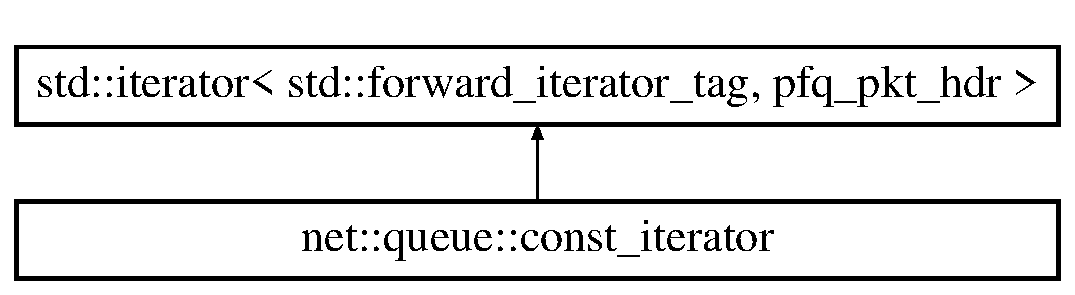
\includegraphics[height=2.000000cm]{structnet_1_1queue_1_1const__iterator}
\end{center}
\end{figure}
\subsection*{Public Member Functions}
\begin{DoxyCompactItemize}
\item 
\hyperlink{structnet_1_1queue_1_1const__iterator_a18317b1de034fe3b5f772a82769bc529}{const\-\_\-iterator} (pfq\-\_\-pkt\-\_\-hdr $\ast$h, size\-\_\-t \hyperlink{classnet_1_1queue_a2c7afc4348eac62342496a735280f265}{slot\-\_\-size}, size\-\_\-t \hyperlink{classnet_1_1queue_a74abf50853b60b5562f12d2294474e59}{index})
\item 
\hyperlink{structnet_1_1queue_1_1const__iterator_a1eea657f0e331d07564147aa3ba2816b}{const\-\_\-iterator} (const \hyperlink{structnet_1_1queue_1_1const__iterator}{const\-\_\-iterator} \&other)
\item 
\hyperlink{structnet_1_1queue_1_1const__iterator_aa20b0a5cfd5c93f04f84793dd0bc7bc3}{const\-\_\-iterator} (const \hyperlink{structnet_1_1queue_1_1iterator}{queue\-::iterator} \&other)
\item 
\hyperlink{structnet_1_1queue_1_1const__iterator_a3cf353d6ca8299a5de48fb2098b5d75e}{$\sim$const\-\_\-iterator} ()=default
\item 
\hyperlink{structnet_1_1queue_1_1const__iterator}{const\-\_\-iterator} \& \hyperlink{structnet_1_1queue_1_1const__iterator_a82607969bb7531adf6647504e6d688b6}{operator++} ()
\item 
\hyperlink{structnet_1_1queue_1_1const__iterator}{const\-\_\-iterator} \hyperlink{structnet_1_1queue_1_1const__iterator_a767a228c684777e2116dac7f4b7de20c}{operator++} (int)
\item 
const pfq\-\_\-pkt\-\_\-hdr $\ast$ \hyperlink{structnet_1_1queue_1_1const__iterator_a632765db721ad2aaa1d37e6398f51116}{operator-\/$>$} () const 
\item 
const pfq\-\_\-pkt\-\_\-hdr \& \hyperlink{structnet_1_1queue_1_1const__iterator_a469c13831f09ed1971b3028dca5f95cf}{operator$\ast$} () const 
\item 
const void $\ast$ \hyperlink{structnet_1_1queue_1_1const__iterator_a68bb9db8a9c3050ec368cd63dce38142}{data} () const 
\item 
bool \hyperlink{structnet_1_1queue_1_1const__iterator_a94ba6cdcfdc81e51a943d5c0d06ba71d}{ready} () const 
\item 
bool \hyperlink{structnet_1_1queue_1_1const__iterator_a9291c46d5ec7d9ca38eb17888dedd9fd}{operator==} (const \hyperlink{structnet_1_1queue_1_1const__iterator}{const\-\_\-iterator} \&other) const 
\item 
bool \hyperlink{structnet_1_1queue_1_1const__iterator_a8c56372b2eaa876c6f857b53a15869e2}{operator!=} (const \hyperlink{structnet_1_1queue_1_1const__iterator}{const\-\_\-iterator} \&other) const 
\end{DoxyCompactItemize}


\subsection{Detailed Description}
Constant forward iterator over packets. 

\subsection{Constructor \& Destructor Documentation}
\hypertarget{structnet_1_1queue_1_1const__iterator_a18317b1de034fe3b5f772a82769bc529}{\index{net\-::queue\-::const\-\_\-iterator@{net\-::queue\-::const\-\_\-iterator}!const\-\_\-iterator@{const\-\_\-iterator}}
\index{const\-\_\-iterator@{const\-\_\-iterator}!net::queue::const_iterator@{net\-::queue\-::const\-\_\-iterator}}
\subsubsection[{const\-\_\-iterator}]{\setlength{\rightskip}{0pt plus 5cm}net\-::queue\-::const\-\_\-iterator\-::const\-\_\-iterator (
\begin{DoxyParamCaption}
\item[{pfq\-\_\-pkt\-\_\-hdr $\ast$}]{h, }
\item[{size\-\_\-t}]{slot\-\_\-size, }
\item[{size\-\_\-t}]{index}
\end{DoxyParamCaption}
)\hspace{0.3cm}{\ttfamily [inline]}}}\label{structnet_1_1queue_1_1const__iterator_a18317b1de034fe3b5f772a82769bc529}
\hypertarget{structnet_1_1queue_1_1const__iterator_a1eea657f0e331d07564147aa3ba2816b}{\index{net\-::queue\-::const\-\_\-iterator@{net\-::queue\-::const\-\_\-iterator}!const\-\_\-iterator@{const\-\_\-iterator}}
\index{const\-\_\-iterator@{const\-\_\-iterator}!net::queue::const_iterator@{net\-::queue\-::const\-\_\-iterator}}
\subsubsection[{const\-\_\-iterator}]{\setlength{\rightskip}{0pt plus 5cm}net\-::queue\-::const\-\_\-iterator\-::const\-\_\-iterator (
\begin{DoxyParamCaption}
\item[{const {\bf const\-\_\-iterator} \&}]{other}
\end{DoxyParamCaption}
)\hspace{0.3cm}{\ttfamily [inline]}}}\label{structnet_1_1queue_1_1const__iterator_a1eea657f0e331d07564147aa3ba2816b}
\hypertarget{structnet_1_1queue_1_1const__iterator_aa20b0a5cfd5c93f04f84793dd0bc7bc3}{\index{net\-::queue\-::const\-\_\-iterator@{net\-::queue\-::const\-\_\-iterator}!const\-\_\-iterator@{const\-\_\-iterator}}
\index{const\-\_\-iterator@{const\-\_\-iterator}!net::queue::const_iterator@{net\-::queue\-::const\-\_\-iterator}}
\subsubsection[{const\-\_\-iterator}]{\setlength{\rightskip}{0pt plus 5cm}net\-::queue\-::const\-\_\-iterator\-::const\-\_\-iterator (
\begin{DoxyParamCaption}
\item[{const {\bf queue\-::iterator} \&}]{other}
\end{DoxyParamCaption}
)\hspace{0.3cm}{\ttfamily [inline]}}}\label{structnet_1_1queue_1_1const__iterator_aa20b0a5cfd5c93f04f84793dd0bc7bc3}
\hypertarget{structnet_1_1queue_1_1const__iterator_a3cf353d6ca8299a5de48fb2098b5d75e}{\index{net\-::queue\-::const\-\_\-iterator@{net\-::queue\-::const\-\_\-iterator}!$\sim$const\-\_\-iterator@{$\sim$const\-\_\-iterator}}
\index{$\sim$const\-\_\-iterator@{$\sim$const\-\_\-iterator}!net::queue::const_iterator@{net\-::queue\-::const\-\_\-iterator}}
\subsubsection[{$\sim$const\-\_\-iterator}]{\setlength{\rightskip}{0pt plus 5cm}net\-::queue\-::const\-\_\-iterator\-::$\sim$const\-\_\-iterator (
\begin{DoxyParamCaption}
{}
\end{DoxyParamCaption}
)\hspace{0.3cm}{\ttfamily [default]}}}\label{structnet_1_1queue_1_1const__iterator_a3cf353d6ca8299a5de48fb2098b5d75e}


\subsection{Member Function Documentation}
\hypertarget{structnet_1_1queue_1_1const__iterator_a68bb9db8a9c3050ec368cd63dce38142}{\index{net\-::queue\-::const\-\_\-iterator@{net\-::queue\-::const\-\_\-iterator}!data@{data}}
\index{data@{data}!net::queue::const_iterator@{net\-::queue\-::const\-\_\-iterator}}
\subsubsection[{data}]{\setlength{\rightskip}{0pt plus 5cm}const void$\ast$ net\-::queue\-::const\-\_\-iterator\-::data (
\begin{DoxyParamCaption}
{}
\end{DoxyParamCaption}
) const\hspace{0.3cm}{\ttfamily [inline]}}}\label{structnet_1_1queue_1_1const__iterator_a68bb9db8a9c3050ec368cd63dce38142}
\hypertarget{structnet_1_1queue_1_1const__iterator_a8c56372b2eaa876c6f857b53a15869e2}{\index{net\-::queue\-::const\-\_\-iterator@{net\-::queue\-::const\-\_\-iterator}!operator!=@{operator!=}}
\index{operator!=@{operator!=}!net::queue::const_iterator@{net\-::queue\-::const\-\_\-iterator}}
\subsubsection[{operator!=}]{\setlength{\rightskip}{0pt plus 5cm}bool net\-::queue\-::const\-\_\-iterator\-::operator!= (
\begin{DoxyParamCaption}
\item[{const {\bf const\-\_\-iterator} \&}]{other}
\end{DoxyParamCaption}
) const\hspace{0.3cm}{\ttfamily [inline]}}}\label{structnet_1_1queue_1_1const__iterator_a8c56372b2eaa876c6f857b53a15869e2}
\hypertarget{structnet_1_1queue_1_1const__iterator_a469c13831f09ed1971b3028dca5f95cf}{\index{net\-::queue\-::const\-\_\-iterator@{net\-::queue\-::const\-\_\-iterator}!operator$\ast$@{operator$\ast$}}
\index{operator$\ast$@{operator$\ast$}!net::queue::const_iterator@{net\-::queue\-::const\-\_\-iterator}}
\subsubsection[{operator$\ast$}]{\setlength{\rightskip}{0pt plus 5cm}const pfq\-\_\-pkt\-\_\-hdr\& net\-::queue\-::const\-\_\-iterator\-::operator$\ast$ (
\begin{DoxyParamCaption}
{}
\end{DoxyParamCaption}
) const\hspace{0.3cm}{\ttfamily [inline]}}}\label{structnet_1_1queue_1_1const__iterator_a469c13831f09ed1971b3028dca5f95cf}
\hypertarget{structnet_1_1queue_1_1const__iterator_a82607969bb7531adf6647504e6d688b6}{\index{net\-::queue\-::const\-\_\-iterator@{net\-::queue\-::const\-\_\-iterator}!operator++@{operator++}}
\index{operator++@{operator++}!net::queue::const_iterator@{net\-::queue\-::const\-\_\-iterator}}
\subsubsection[{operator++}]{\setlength{\rightskip}{0pt plus 5cm}{\bf const\-\_\-iterator}\& net\-::queue\-::const\-\_\-iterator\-::operator++ (
\begin{DoxyParamCaption}
{}
\end{DoxyParamCaption}
)\hspace{0.3cm}{\ttfamily [inline]}}}\label{structnet_1_1queue_1_1const__iterator_a82607969bb7531adf6647504e6d688b6}
\hypertarget{structnet_1_1queue_1_1const__iterator_a767a228c684777e2116dac7f4b7de20c}{\index{net\-::queue\-::const\-\_\-iterator@{net\-::queue\-::const\-\_\-iterator}!operator++@{operator++}}
\index{operator++@{operator++}!net::queue::const_iterator@{net\-::queue\-::const\-\_\-iterator}}
\subsubsection[{operator++}]{\setlength{\rightskip}{0pt plus 5cm}{\bf const\-\_\-iterator} net\-::queue\-::const\-\_\-iterator\-::operator++ (
\begin{DoxyParamCaption}
\item[{int}]{}
\end{DoxyParamCaption}
)\hspace{0.3cm}{\ttfamily [inline]}}}\label{structnet_1_1queue_1_1const__iterator_a767a228c684777e2116dac7f4b7de20c}
\hypertarget{structnet_1_1queue_1_1const__iterator_a632765db721ad2aaa1d37e6398f51116}{\index{net\-::queue\-::const\-\_\-iterator@{net\-::queue\-::const\-\_\-iterator}!operator-\/$>$@{operator-\/$>$}}
\index{operator-\/$>$@{operator-\/$>$}!net::queue::const_iterator@{net\-::queue\-::const\-\_\-iterator}}
\subsubsection[{operator-\/$>$}]{\setlength{\rightskip}{0pt plus 5cm}const pfq\-\_\-pkt\-\_\-hdr$\ast$ net\-::queue\-::const\-\_\-iterator\-::operator-\/$>$ (
\begin{DoxyParamCaption}
{}
\end{DoxyParamCaption}
) const\hspace{0.3cm}{\ttfamily [inline]}}}\label{structnet_1_1queue_1_1const__iterator_a632765db721ad2aaa1d37e6398f51116}
\hypertarget{structnet_1_1queue_1_1const__iterator_a9291c46d5ec7d9ca38eb17888dedd9fd}{\index{net\-::queue\-::const\-\_\-iterator@{net\-::queue\-::const\-\_\-iterator}!operator==@{operator==}}
\index{operator==@{operator==}!net::queue::const_iterator@{net\-::queue\-::const\-\_\-iterator}}
\subsubsection[{operator==}]{\setlength{\rightskip}{0pt plus 5cm}bool net\-::queue\-::const\-\_\-iterator\-::operator== (
\begin{DoxyParamCaption}
\item[{const {\bf const\-\_\-iterator} \&}]{other}
\end{DoxyParamCaption}
) const\hspace{0.3cm}{\ttfamily [inline]}}}\label{structnet_1_1queue_1_1const__iterator_a9291c46d5ec7d9ca38eb17888dedd9fd}
\hypertarget{structnet_1_1queue_1_1const__iterator_a94ba6cdcfdc81e51a943d5c0d06ba71d}{\index{net\-::queue\-::const\-\_\-iterator@{net\-::queue\-::const\-\_\-iterator}!ready@{ready}}
\index{ready@{ready}!net::queue::const_iterator@{net\-::queue\-::const\-\_\-iterator}}
\subsubsection[{ready}]{\setlength{\rightskip}{0pt plus 5cm}bool net\-::queue\-::const\-\_\-iterator\-::ready (
\begin{DoxyParamCaption}
{}
\end{DoxyParamCaption}
) const\hspace{0.3cm}{\ttfamily [inline]}}}\label{structnet_1_1queue_1_1const__iterator_a94ba6cdcfdc81e51a943d5c0d06ba71d}


The documentation for this struct was generated from the following file\-:\begin{DoxyCompactItemize}
\item 
C++/\hyperlink{pfq-queue_8hpp}{pfq-\/queue.\-hpp}\end{DoxyCompactItemize}

\hypertarget{structnet_1_1queue_1_1iterator}{\section{net\-:\-:queue\-:\-:iterator Struct Reference}
\label{structnet_1_1queue_1_1iterator}\index{net\-::queue\-::iterator@{net\-::queue\-::iterator}}
}


Forward iterator over packets.  




{\ttfamily \#include $<$pfq-\/queue.\-hpp$>$}

Inheritance diagram for net\-:\-:queue\-:\-:iterator\-:\begin{figure}[H]
\begin{center}
\leavevmode
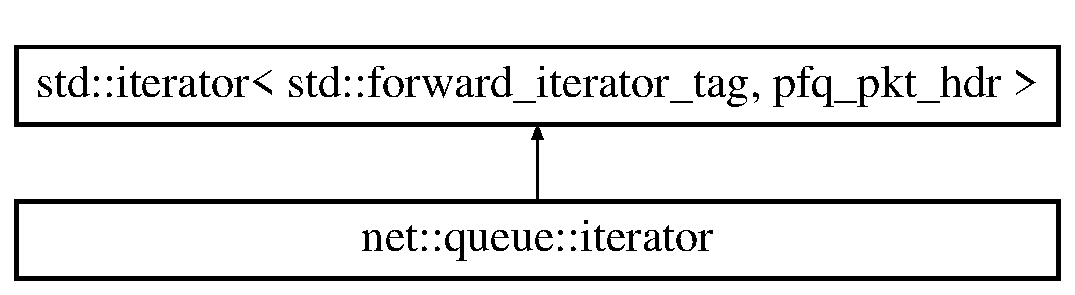
\includegraphics[height=2.000000cm]{structnet_1_1queue_1_1iterator}
\end{center}
\end{figure}
\subsection*{Public Member Functions}
\begin{DoxyCompactItemize}
\item 
\hyperlink{structnet_1_1queue_1_1iterator_ab8056bf9450fb09098212d643ec60165}{iterator} (pfq\-\_\-pkt\-\_\-hdr $\ast$h, size\-\_\-t \hyperlink{classnet_1_1queue_a2c7afc4348eac62342496a735280f265}{slot\-\_\-size}, size\-\_\-t \hyperlink{classnet_1_1queue_a74abf50853b60b5562f12d2294474e59}{index})
\item 
\hyperlink{structnet_1_1queue_1_1iterator_a4561340ab7b2bf535c3c90ec15328426}{$\sim$iterator} ()=default
\item 
\hyperlink{structnet_1_1queue_1_1iterator_a781befe661b1bd046751ccb336fc2556}{iterator} (const \hyperlink{structnet_1_1queue_1_1iterator}{iterator} \&other)
\item 
\hyperlink{structnet_1_1queue_1_1iterator}{iterator} \& \hyperlink{structnet_1_1queue_1_1iterator_a51484c9699f5fe3d9df7961570de3f6b}{operator++} ()
\item 
\hyperlink{structnet_1_1queue_1_1iterator}{iterator} \hyperlink{structnet_1_1queue_1_1iterator_ac14b5df947132a5151b485772c7f50d6}{operator++} (int)
\item 
pfq\-\_\-pkt\-\_\-hdr $\ast$ \hyperlink{structnet_1_1queue_1_1iterator_acc9649d5c628ae6325f657c9058cb515}{operator-\/$>$} () const 
\item 
pfq\-\_\-pkt\-\_\-hdr \& \hyperlink{structnet_1_1queue_1_1iterator_a44627e99c3e88002d803c975bec64709}{operator$\ast$} () const 
\item 
void $\ast$ \hyperlink{structnet_1_1queue_1_1iterator_a70cbc265b9060fb889494e7b9940354f}{data} () const 
\item 
bool \hyperlink{structnet_1_1queue_1_1iterator_a8b5eb1e998c775de8066ee2063d94b47}{ready} () const 
\item 
bool \hyperlink{structnet_1_1queue_1_1iterator_a18ac00a8ff6db4be086ac8fddc7451c2}{operator==} (const \hyperlink{structnet_1_1queue_1_1iterator}{iterator} \&other) const 
\item 
bool \hyperlink{structnet_1_1queue_1_1iterator_a9cf0fa72ce3994c3c1625d59b0f08b77}{operator!=} (const \hyperlink{structnet_1_1queue_1_1iterator}{iterator} \&other) const 
\end{DoxyCompactItemize}
\subsection*{Friends}
\begin{DoxyCompactItemize}
\item 
struct \hyperlink{structnet_1_1queue_1_1iterator_a58a3589426e806d3416f369707f00b70}{queue\-::const\-\_\-iterator}
\end{DoxyCompactItemize}


\subsection{Detailed Description}
Forward iterator over packets. 

\subsection{Constructor \& Destructor Documentation}
\hypertarget{structnet_1_1queue_1_1iterator_ab8056bf9450fb09098212d643ec60165}{\index{net\-::queue\-::iterator@{net\-::queue\-::iterator}!iterator@{iterator}}
\index{iterator@{iterator}!net::queue::iterator@{net\-::queue\-::iterator}}
\subsubsection[{iterator}]{\setlength{\rightskip}{0pt plus 5cm}net\-::queue\-::iterator\-::iterator (
\begin{DoxyParamCaption}
\item[{pfq\-\_\-pkt\-\_\-hdr $\ast$}]{h, }
\item[{size\-\_\-t}]{slot\-\_\-size, }
\item[{size\-\_\-t}]{index}
\end{DoxyParamCaption}
)\hspace{0.3cm}{\ttfamily [inline]}}}\label{structnet_1_1queue_1_1iterator_ab8056bf9450fb09098212d643ec60165}
\hypertarget{structnet_1_1queue_1_1iterator_a4561340ab7b2bf535c3c90ec15328426}{\index{net\-::queue\-::iterator@{net\-::queue\-::iterator}!$\sim$iterator@{$\sim$iterator}}
\index{$\sim$iterator@{$\sim$iterator}!net::queue::iterator@{net\-::queue\-::iterator}}
\subsubsection[{$\sim$iterator}]{\setlength{\rightskip}{0pt plus 5cm}net\-::queue\-::iterator\-::$\sim$iterator (
\begin{DoxyParamCaption}
{}
\end{DoxyParamCaption}
)\hspace{0.3cm}{\ttfamily [default]}}}\label{structnet_1_1queue_1_1iterator_a4561340ab7b2bf535c3c90ec15328426}
\hypertarget{structnet_1_1queue_1_1iterator_a781befe661b1bd046751ccb336fc2556}{\index{net\-::queue\-::iterator@{net\-::queue\-::iterator}!iterator@{iterator}}
\index{iterator@{iterator}!net::queue::iterator@{net\-::queue\-::iterator}}
\subsubsection[{iterator}]{\setlength{\rightskip}{0pt plus 5cm}net\-::queue\-::iterator\-::iterator (
\begin{DoxyParamCaption}
\item[{const {\bf iterator} \&}]{other}
\end{DoxyParamCaption}
)\hspace{0.3cm}{\ttfamily [inline]}}}\label{structnet_1_1queue_1_1iterator_a781befe661b1bd046751ccb336fc2556}


\subsection{Member Function Documentation}
\hypertarget{structnet_1_1queue_1_1iterator_a70cbc265b9060fb889494e7b9940354f}{\index{net\-::queue\-::iterator@{net\-::queue\-::iterator}!data@{data}}
\index{data@{data}!net::queue::iterator@{net\-::queue\-::iterator}}
\subsubsection[{data}]{\setlength{\rightskip}{0pt plus 5cm}void$\ast$ net\-::queue\-::iterator\-::data (
\begin{DoxyParamCaption}
{}
\end{DoxyParamCaption}
) const\hspace{0.3cm}{\ttfamily [inline]}}}\label{structnet_1_1queue_1_1iterator_a70cbc265b9060fb889494e7b9940354f}
\hypertarget{structnet_1_1queue_1_1iterator_a9cf0fa72ce3994c3c1625d59b0f08b77}{\index{net\-::queue\-::iterator@{net\-::queue\-::iterator}!operator!=@{operator!=}}
\index{operator!=@{operator!=}!net::queue::iterator@{net\-::queue\-::iterator}}
\subsubsection[{operator!=}]{\setlength{\rightskip}{0pt plus 5cm}bool net\-::queue\-::iterator\-::operator!= (
\begin{DoxyParamCaption}
\item[{const {\bf iterator} \&}]{other}
\end{DoxyParamCaption}
) const\hspace{0.3cm}{\ttfamily [inline]}}}\label{structnet_1_1queue_1_1iterator_a9cf0fa72ce3994c3c1625d59b0f08b77}
\hypertarget{structnet_1_1queue_1_1iterator_a44627e99c3e88002d803c975bec64709}{\index{net\-::queue\-::iterator@{net\-::queue\-::iterator}!operator$\ast$@{operator$\ast$}}
\index{operator$\ast$@{operator$\ast$}!net::queue::iterator@{net\-::queue\-::iterator}}
\subsubsection[{operator$\ast$}]{\setlength{\rightskip}{0pt plus 5cm}pfq\-\_\-pkt\-\_\-hdr\& net\-::queue\-::iterator\-::operator$\ast$ (
\begin{DoxyParamCaption}
{}
\end{DoxyParamCaption}
) const\hspace{0.3cm}{\ttfamily [inline]}}}\label{structnet_1_1queue_1_1iterator_a44627e99c3e88002d803c975bec64709}
\hypertarget{structnet_1_1queue_1_1iterator_a51484c9699f5fe3d9df7961570de3f6b}{\index{net\-::queue\-::iterator@{net\-::queue\-::iterator}!operator++@{operator++}}
\index{operator++@{operator++}!net::queue::iterator@{net\-::queue\-::iterator}}
\subsubsection[{operator++}]{\setlength{\rightskip}{0pt plus 5cm}{\bf iterator}\& net\-::queue\-::iterator\-::operator++ (
\begin{DoxyParamCaption}
{}
\end{DoxyParamCaption}
)\hspace{0.3cm}{\ttfamily [inline]}}}\label{structnet_1_1queue_1_1iterator_a51484c9699f5fe3d9df7961570de3f6b}
\hypertarget{structnet_1_1queue_1_1iterator_ac14b5df947132a5151b485772c7f50d6}{\index{net\-::queue\-::iterator@{net\-::queue\-::iterator}!operator++@{operator++}}
\index{operator++@{operator++}!net::queue::iterator@{net\-::queue\-::iterator}}
\subsubsection[{operator++}]{\setlength{\rightskip}{0pt plus 5cm}{\bf iterator} net\-::queue\-::iterator\-::operator++ (
\begin{DoxyParamCaption}
\item[{int}]{}
\end{DoxyParamCaption}
)\hspace{0.3cm}{\ttfamily [inline]}}}\label{structnet_1_1queue_1_1iterator_ac14b5df947132a5151b485772c7f50d6}
\hypertarget{structnet_1_1queue_1_1iterator_acc9649d5c628ae6325f657c9058cb515}{\index{net\-::queue\-::iterator@{net\-::queue\-::iterator}!operator-\/$>$@{operator-\/$>$}}
\index{operator-\/$>$@{operator-\/$>$}!net::queue::iterator@{net\-::queue\-::iterator}}
\subsubsection[{operator-\/$>$}]{\setlength{\rightskip}{0pt plus 5cm}pfq\-\_\-pkt\-\_\-hdr$\ast$ net\-::queue\-::iterator\-::operator-\/$>$ (
\begin{DoxyParamCaption}
{}
\end{DoxyParamCaption}
) const\hspace{0.3cm}{\ttfamily [inline]}}}\label{structnet_1_1queue_1_1iterator_acc9649d5c628ae6325f657c9058cb515}
\hypertarget{structnet_1_1queue_1_1iterator_a18ac00a8ff6db4be086ac8fddc7451c2}{\index{net\-::queue\-::iterator@{net\-::queue\-::iterator}!operator==@{operator==}}
\index{operator==@{operator==}!net::queue::iterator@{net\-::queue\-::iterator}}
\subsubsection[{operator==}]{\setlength{\rightskip}{0pt plus 5cm}bool net\-::queue\-::iterator\-::operator== (
\begin{DoxyParamCaption}
\item[{const {\bf iterator} \&}]{other}
\end{DoxyParamCaption}
) const\hspace{0.3cm}{\ttfamily [inline]}}}\label{structnet_1_1queue_1_1iterator_a18ac00a8ff6db4be086ac8fddc7451c2}
\hypertarget{structnet_1_1queue_1_1iterator_a8b5eb1e998c775de8066ee2063d94b47}{\index{net\-::queue\-::iterator@{net\-::queue\-::iterator}!ready@{ready}}
\index{ready@{ready}!net::queue::iterator@{net\-::queue\-::iterator}}
\subsubsection[{ready}]{\setlength{\rightskip}{0pt plus 5cm}bool net\-::queue\-::iterator\-::ready (
\begin{DoxyParamCaption}
{}
\end{DoxyParamCaption}
) const\hspace{0.3cm}{\ttfamily [inline]}}}\label{structnet_1_1queue_1_1iterator_a8b5eb1e998c775de8066ee2063d94b47}


\subsection{Friends And Related Function Documentation}
\hypertarget{structnet_1_1queue_1_1iterator_a58a3589426e806d3416f369707f00b70}{\index{net\-::queue\-::iterator@{net\-::queue\-::iterator}!queue\-::const\-\_\-iterator@{queue\-::const\-\_\-iterator}}
\index{queue\-::const\-\_\-iterator@{queue\-::const\-\_\-iterator}!net::queue::iterator@{net\-::queue\-::iterator}}
\subsubsection[{queue\-::const\-\_\-iterator}]{\setlength{\rightskip}{0pt plus 5cm}friend struct {\bf queue\-::const\-\_\-iterator}\hspace{0.3cm}{\ttfamily [friend]}}}\label{structnet_1_1queue_1_1iterator_a58a3589426e806d3416f369707f00b70}


The documentation for this struct was generated from the following file\-:\begin{DoxyCompactItemize}
\item 
/root/\-Git\-Hub/\-P\-F\-Q/user/\-C++/\hyperlink{pfq-queue_8hpp}{pfq-\/queue.\-hpp}\end{DoxyCompactItemize}

\hypertarget{structnet_1_1param_1_1maxlen}{\section{net\+:\+:param\+:\+:maxlen Struct Reference}
\label{structnet_1_1param_1_1maxlen}\index{net\+::param\+::maxlen@{net\+::param\+::maxlen}}
}


{\ttfamily \#include $<$pfq.\+hpp$>$}

\subsection*{Public Attributes}
\begin{DoxyCompactItemize}
\item 
size\+\_\+t \hyperlink{structnet_1_1param_1_1maxlen_aa6980872f44af9803747a76004a1c55a}{value}
\end{DoxyCompactItemize}


\subsection{Member Data Documentation}
\hypertarget{structnet_1_1param_1_1maxlen_aa6980872f44af9803747a76004a1c55a}{\index{net\+::param\+::maxlen@{net\+::param\+::maxlen}!value@{value}}
\index{value@{value}!net\+::param\+::maxlen@{net\+::param\+::maxlen}}
\subsubsection[{value}]{\setlength{\rightskip}{0pt plus 5cm}size\+\_\+t net\+::param\+::maxlen\+::value}}\label{structnet_1_1param_1_1maxlen_aa6980872f44af9803747a76004a1c55a}


The documentation for this struct was generated from the following file\+:\begin{DoxyCompactItemize}
\item 
C++/\hyperlink{pfq_8hpp}{pfq.\+hpp}\end{DoxyCompactItemize}

\hypertarget{classnet_1_1pfq}{\section{net\-:\-:pfq Class Reference}
\label{classnet_1_1pfq}\index{net\-::pfq@{net\-::pfq}}
}


P\-F\-Q\-: the class.  




{\ttfamily \#include $<$pfq.\-hpp$>$}

\subsection*{Public Member Functions}
\begin{DoxyCompactItemize}
\item 
\hyperlink{classnet_1_1pfq_a43214f93ed81a6344c83f991cb1311a7}{pfq} ()
\begin{DoxyCompactList}\small\item\em Default constructor. \end{DoxyCompactList}\item 
{\footnotesize template$<$typename... Ts$>$ }\\\hyperlink{classnet_1_1pfq_a886761849ccf9b22d3eac521c67a89ab}{pfq} (param\-::list\-\_\-t, Ts \&\&...args)
\begin{DoxyCompactList}\small\item\em Constructor with named-\/parameter idiom (\hyperlink{namespacenet_1_1param_a9020a1d5f00da972acbea3e809d3c602}{param\-::get} is the C++14 std\-::get) \end{DoxyCompactList}\item 
\hyperlink{classnet_1_1pfq_af9794841bcf6982000538da4f9ffb824}{pfq} (size\-\_\-t \hyperlink{classnet_1_1pfq_aa915603b2ad8d1226f9bbea0050945c0}{caplen}, size\-\_\-t \hyperlink{classnet_1_1pfq_a83ed78c8c7bc2de33e75e244bbc0b603}{offset}=0, size\-\_\-t \hyperlink{classnet_1_1pfq_a878c768492c68fc572a994a58913a3db}{rx\-\_\-slots}=65536, size\-\_\-t \hyperlink{classnet_1_1pfq_a0424e39990711493af4f24a0c3e9be4d}{maxlen}=64, size\-\_\-t \hyperlink{classnet_1_1pfq_aae98015b961c6210081fa29a2ea34da2}{tx\-\_\-slots}=4096)
\begin{DoxyCompactList}\small\item\em Constructor. \end{DoxyCompactList}\item 
\hyperlink{classnet_1_1pfq_a845ec21f53fd0fbc396b4b682227caa4}{pfq} (\hyperlink{namespacenet_aedc1a0dde937ddbd0800af02920b1067}{group\-\_\-policy} policy, size\-\_\-t \hyperlink{classnet_1_1pfq_aa915603b2ad8d1226f9bbea0050945c0}{caplen}, size\-\_\-t \hyperlink{classnet_1_1pfq_a83ed78c8c7bc2de33e75e244bbc0b603}{offset}=0, size\-\_\-t \hyperlink{classnet_1_1pfq_a878c768492c68fc572a994a58913a3db}{rx\-\_\-slots}=65536, size\-\_\-t \hyperlink{classnet_1_1pfq_a0424e39990711493af4f24a0c3e9be4d}{maxlen}=64, size\-\_\-t \hyperlink{classnet_1_1pfq_aae98015b961c6210081fa29a2ea34da2}{tx\-\_\-slots}=4096)
\begin{DoxyCompactList}\small\item\em Constructor. \end{DoxyCompactList}\item 
\hyperlink{classnet_1_1pfq_a829b17b7f6b5471512a05003c77c68e2}{pfq} (\hyperlink{namespacenet_a1dbd93552dc6ef6fbb0bb79d43ca22fd}{class\-\_\-mask} mask, \hyperlink{namespacenet_aedc1a0dde937ddbd0800af02920b1067}{group\-\_\-policy} policy, size\-\_\-t \hyperlink{classnet_1_1pfq_aa915603b2ad8d1226f9bbea0050945c0}{caplen}, size\-\_\-t \hyperlink{classnet_1_1pfq_a83ed78c8c7bc2de33e75e244bbc0b603}{offset}=0, size\-\_\-t \hyperlink{classnet_1_1pfq_a878c768492c68fc572a994a58913a3db}{rx\-\_\-slots}=65536, size\-\_\-t \hyperlink{classnet_1_1pfq_a0424e39990711493af4f24a0c3e9be4d}{maxlen}=64, size\-\_\-t \hyperlink{classnet_1_1pfq_aae98015b961c6210081fa29a2ea34da2}{tx\-\_\-slots}=4096)
\begin{DoxyCompactList}\small\item\em Constructor. \end{DoxyCompactList}\item 
\hyperlink{classnet_1_1pfq_acf552123cd0e53eb5b96a4e1eb1b50a2}{$\sim$pfq} ()
\begin{DoxyCompactList}\small\item\em Destructor\-: close the socket. \end{DoxyCompactList}\item 
\hyperlink{classnet_1_1pfq_aafcf0308f9f4a0da319b8b688b2ad3a9}{pfq} (const \hyperlink{classnet_1_1pfq}{pfq} \&)=delete
\begin{DoxyCompactList}\small\item\em P\-F\-Q socket is a non-\/copyable resource. \end{DoxyCompactList}\item 
\hyperlink{classnet_1_1pfq}{pfq} \& \hyperlink{classnet_1_1pfq_a6a00af55f2109382c2cc20a47da43623}{operator=} (const \hyperlink{classnet_1_1pfq}{pfq} \&)=delete
\begin{DoxyCompactList}\small\item\em P\-F\-Q socket is a non-\/copy assignable resource. \end{DoxyCompactList}\item 
\hyperlink{classnet_1_1pfq_acce7496d2c4308539cc0360793683acd}{pfq} (\hyperlink{classnet_1_1pfq}{pfq} \&\&other) noexcept
\begin{DoxyCompactList}\small\item\em Move constructor. \end{DoxyCompactList}\item 
\hyperlink{classnet_1_1pfq}{pfq} \& \hyperlink{classnet_1_1pfq_aeacd42c1616840fa20e67bbf47c71e70}{operator=} (\hyperlink{classnet_1_1pfq}{pfq} \&\&other) noexcept
\begin{DoxyCompactList}\small\item\em Move assignment operator. \end{DoxyCompactList}\item 
void \hyperlink{classnet_1_1pfq_a762b45c2020a73e503cdbc2b4631db1c}{swap} (\hyperlink{classnet_1_1pfq}{pfq} \&other)
\begin{DoxyCompactList}\small\item\em Swap two P\-F\-Q sockets. \end{DoxyCompactList}\item 
void \hyperlink{classnet_1_1pfq_a100388ca866fb38102a8d96581f1f16d}{open} (\hyperlink{namespacenet_aedc1a0dde937ddbd0800af02920b1067}{group\-\_\-policy} policy, size\-\_\-t \hyperlink{classnet_1_1pfq_aa915603b2ad8d1226f9bbea0050945c0}{caplen}, size\-\_\-t \hyperlink{classnet_1_1pfq_a83ed78c8c7bc2de33e75e244bbc0b603}{offset}=0, size\-\_\-t \hyperlink{classnet_1_1pfq_a878c768492c68fc572a994a58913a3db}{rx\-\_\-slots}=65536, size\-\_\-t \hyperlink{classnet_1_1pfq_a0424e39990711493af4f24a0c3e9be4d}{maxlen}=64, size\-\_\-t \hyperlink{classnet_1_1pfq_aae98015b961c6210081fa29a2ea34da2}{tx\-\_\-slots}=4096)
\begin{DoxyCompactList}\small\item\em Open the P\-F\-Q socket with the given group policy. \end{DoxyCompactList}\item 
void \hyperlink{classnet_1_1pfq_a99183f977ae2dcfa2788b9f1a7f29097}{open} (\hyperlink{namespacenet_a1dbd93552dc6ef6fbb0bb79d43ca22fd}{class\-\_\-mask} mask, \hyperlink{namespacenet_aedc1a0dde937ddbd0800af02920b1067}{group\-\_\-policy} policy, size\-\_\-t \hyperlink{classnet_1_1pfq_aa915603b2ad8d1226f9bbea0050945c0}{caplen}, size\-\_\-t \hyperlink{classnet_1_1pfq_a83ed78c8c7bc2de33e75e244bbc0b603}{offset}=0, size\-\_\-t \hyperlink{classnet_1_1pfq_a878c768492c68fc572a994a58913a3db}{rx\-\_\-slots}=65536, size\-\_\-t \hyperlink{classnet_1_1pfq_a0424e39990711493af4f24a0c3e9be4d}{maxlen}=64, size\-\_\-t \hyperlink{classnet_1_1pfq_aae98015b961c6210081fa29a2ea34da2}{tx\-\_\-slots}=4096)
\begin{DoxyCompactList}\small\item\em Open the P\-F\-Q socket with the given class mask and group policy. \end{DoxyCompactList}\item 
{\footnotesize template$<$typename... Ts$>$ }\\void \hyperlink{classnet_1_1pfq_a5e435f3be2e02f3eeb73aad94f2fe27c}{open} (param\-::list\-\_\-t, Ts \&\&...args)
\begin{DoxyCompactList}\small\item\em Open the socket with named-\/parameter idiom. \end{DoxyCompactList}\item 
int \hyperlink{classnet_1_1pfq_a9ee042216fa93f524050a10a195935a3}{id} () const 
\begin{DoxyCompactList}\small\item\em Return the id for the socket. \end{DoxyCompactList}\item 
int \hyperlink{classnet_1_1pfq_a804ef7e3c673827799c6ade879fe5760}{group\-\_\-id} () const 
\begin{DoxyCompactList}\small\item\em Return the group-\/id for the socket. \end{DoxyCompactList}\item 
int \hyperlink{classnet_1_1pfq_a9a824d52bd660d12700f8475f04230dd}{fd} () const 
\begin{DoxyCompactList}\small\item\em Return the underlying file descriptor. \end{DoxyCompactList}\item 
void \hyperlink{classnet_1_1pfq_a3b96eb3ab597bc88142239fa840dbbe0}{close} ()
\begin{DoxyCompactList}\small\item\em Close the socket. \end{DoxyCompactList}\item 
void \hyperlink{classnet_1_1pfq_a503deb297624d708efe3ed2e4ae0a3ef}{enable} ()
\begin{DoxyCompactList}\small\item\em Enable the socket for packet capture. \end{DoxyCompactList}\item 
void \hyperlink{classnet_1_1pfq_a2396ccadb0f467760355f352fdc9d989}{disable} ()
\begin{DoxyCompactList}\small\item\em Disable the packet capture. \end{DoxyCompactList}\item 
bool \hyperlink{classnet_1_1pfq_ac1dd1a25c65ff07d8ad4d681dc0633c8}{enabled} () const 
\begin{DoxyCompactList}\small\item\em Check whether the packet capture is enabled. \end{DoxyCompactList}\item 
void \hyperlink{classnet_1_1pfq_ac8dc23932b27dd04c8ecbdcbabe931b8}{timestamp\-\_\-enable} (bool value)
\begin{DoxyCompactList}\small\item\em Turn on/off the timestamp for packets. \end{DoxyCompactList}\item 
bool \hyperlink{classnet_1_1pfq_a7939df6cf5127dd8672e1ca0a68fa648}{timestamp\-\_\-enabled} () const 
\begin{DoxyCompactList}\small\item\em Check whether the timestamp is enabled for packets. \end{DoxyCompactList}\item 
void \hyperlink{classnet_1_1pfq_aa915603b2ad8d1226f9bbea0050945c0}{caplen} (size\-\_\-t value)
\begin{DoxyCompactList}\small\item\em Set the capture length of packets in bytes. \end{DoxyCompactList}\item 
size\-\_\-t \hyperlink{classnet_1_1pfq_aa0d64b89a345ca5426a694f6583106c3}{caplen} () const 
\begin{DoxyCompactList}\small\item\em Get the capture length of packets. \end{DoxyCompactList}\item 
void \hyperlink{classnet_1_1pfq_a0424e39990711493af4f24a0c3e9be4d}{maxlen} (size\-\_\-t value)
\begin{DoxyCompactList}\small\item\em Set the max transmission length of packets in bytes. \end{DoxyCompactList}\item 
size\-\_\-t \hyperlink{classnet_1_1pfq_a869695c441902d0342212d7581f3e362}{maxlen} () const 
\begin{DoxyCompactList}\small\item\em Get the max transmission length of packets. \end{DoxyCompactList}\item 
void \hyperlink{classnet_1_1pfq_a83ed78c8c7bc2de33e75e244bbc0b603}{offset} (size\-\_\-t value)
\begin{DoxyCompactList}\small\item\em Set the capture offset of packets, in bytes. \end{DoxyCompactList}\item 
size\-\_\-t \hyperlink{classnet_1_1pfq_ad419e5ef48bb5f9639c798b3d2dd1660}{offset} () const 
\begin{DoxyCompactList}\small\item\em Get the capture offset of packets. \end{DoxyCompactList}\item 
void \hyperlink{classnet_1_1pfq_a878c768492c68fc572a994a58913a3db}{rx\-\_\-slots} (size\-\_\-t value)
\begin{DoxyCompactList}\small\item\em Specify the length of the R\-X queue, in number of packets. \end{DoxyCompactList}\item 
size\-\_\-t \hyperlink{classnet_1_1pfq_aa4382e74b5975f81e5b5f676ed0177bb}{rx\-\_\-slots} () const 
\begin{DoxyCompactList}\small\item\em Get the length of the R\-X queue, in number of packets. \end{DoxyCompactList}\item 
void \hyperlink{classnet_1_1pfq_aae98015b961c6210081fa29a2ea34da2}{tx\-\_\-slots} (size\-\_\-t value)
\begin{DoxyCompactList}\small\item\em Specify the length of the T\-X queue, in number of packets. \end{DoxyCompactList}\item 
size\-\_\-t \hyperlink{classnet_1_1pfq_aea6852bcf02bf2430a6a7fe25131c4ab}{tx\-\_\-slots} () const 
\begin{DoxyCompactList}\small\item\em Get the length of the T\-X queue, in number of packets. \end{DoxyCompactList}\item 
size\-\_\-t \hyperlink{classnet_1_1pfq_a8616d3cd53f1a49ff347cc4599e7c04c}{rx\-\_\-slot\-\_\-size} () const 
\begin{DoxyCompactList}\small\item\em Get the length of a R\-X slot, in bytes. \end{DoxyCompactList}\item 
void \hyperlink{classnet_1_1pfq_a3e55b38d9f094ab88c3510c91a3c8ac5}{bind} (const char $\ast$dev, int \hyperlink{classnet_1_1queue}{queue}=\hyperlink{classnet_1_1pfq_a0d4eca6d0925b7c49365675c9cf9385c}{any\-\_\-queue})
\begin{DoxyCompactList}\small\item\em Bind the group of the socket to the given device/queue. \end{DoxyCompactList}\item 
void \hyperlink{classnet_1_1pfq_a2b8310320db5d583625d67eaae8be047}{bind\-\_\-group} (int gid, const char $\ast$dev, int \hyperlink{classnet_1_1queue}{queue}=\hyperlink{classnet_1_1pfq_a0d4eca6d0925b7c49365675c9cf9385c}{any\-\_\-queue})
\begin{DoxyCompactList}\small\item\em Bind the group to the given device/queue. \end{DoxyCompactList}\item 
void \hyperlink{classnet_1_1pfq_a769e03c88c5cda30f14e67a7a398aac3}{unbind} (const char $\ast$dev, int \hyperlink{classnet_1_1queue}{queue}=\hyperlink{classnet_1_1pfq_a0d4eca6d0925b7c49365675c9cf9385c}{any\-\_\-queue})
\begin{DoxyCompactList}\small\item\em Unbind the group of the socket from the given device/queue. \end{DoxyCompactList}\item 
void \hyperlink{classnet_1_1pfq_a3bbc9de1354d5cd3e99804e55618a1a3}{unbind\-\_\-group} (int gid, const char $\ast$dev, int \hyperlink{classnet_1_1queue}{queue}=\hyperlink{classnet_1_1pfq_a0d4eca6d0925b7c49365675c9cf9385c}{any\-\_\-queue})
\begin{DoxyCompactList}\small\item\em Unbind the group from the given device/queue. \end{DoxyCompactList}\item 
unsigned long \hyperlink{classnet_1_1pfq_a37b9270cf29bb67a4b4e577646b39a78}{groups\-\_\-mask} () const 
\begin{DoxyCompactList}\small\item\em Obtain the mask of the joined groups. \end{DoxyCompactList}\item 
std\-::vector$<$ int $>$ \hyperlink{classnet_1_1pfq_af63de1f94a492284cfed78695f2e93ec}{groups} () const 
\begin{DoxyCompactList}\small\item\em Obtain the list of the joined groups. \end{DoxyCompactList}\item 
{\footnotesize template$<$typename Comp $>$ }\\void \hyperlink{classnet_1_1pfq_af434441b7c824c81e3888f771b70e023}{set\-\_\-group\-\_\-computation} (int gid, Comp const \&comp)
\begin{DoxyCompactList}\small\item\em Specify a functional computation for the given group. \end{DoxyCompactList}\item 
void \hyperlink{classnet_1_1pfq_a50af39653699ccbf9c0b2412a17e01a6}{set\-\_\-group\-\_\-computation} (int gid, pfq\-\_\-computation\-\_\-descr $\ast$prog)
\begin{DoxyCompactList}\small\item\em Specify a functional computation for the given group. \end{DoxyCompactList}\item 
void \hyperlink{classnet_1_1pfq_a5290b64ce270cfc46a9fbecc21802cc3}{set\-\_\-group\-\_\-fprog} (int gid, const sock\-\_\-fprog \&f)
\begin{DoxyCompactList}\small\item\em Specify a B\-P\-F program for the given group. \end{DoxyCompactList}\item 
void \hyperlink{classnet_1_1pfq_a4d6b1fb7c2b3538bf7b66fb0a92bf87b}{reset\-\_\-group\-\_\-fprog} (int gid)
\begin{DoxyCompactList}\small\item\em Reset the B\-P\-F program fro the given group. \end{DoxyCompactList}\item 
int \hyperlink{classnet_1_1pfq_ad7e62e04d59c1f2214ff5314bb6b3825}{join\-\_\-group} (int gid, \hyperlink{namespacenet_aedc1a0dde937ddbd0800af02920b1067}{group\-\_\-policy} pol=\hyperlink{namespacenet_aedc1a0dde937ddbd0800af02920b1067a9e81e7b963c71363e2fb3eefcfecfc0e}{group\-\_\-policy\-::shared}, \hyperlink{namespacenet_a1dbd93552dc6ef6fbb0bb79d43ca22fd}{class\-\_\-mask} mask=\hyperlink{namespacenet_a1dbd93552dc6ef6fbb0bb79d43ca22fda172b03053216c6158fe380805998ad6c}{class\-\_\-mask\-::default\-\_\-})
\begin{DoxyCompactList}\small\item\em Join the given group. \end{DoxyCompactList}\item 
void \hyperlink{classnet_1_1pfq_af90932832d9695326df7af8b2d629660}{leave\-\_\-group} (int gid)
\begin{DoxyCompactList}\small\item\em Leave the given group. \end{DoxyCompactList}\item 
int \hyperlink{classnet_1_1pfq_ae082956072242f6a05a9ba3ab076b59e}{poll} (long int microseconds=-\/1)
\begin{DoxyCompactList}\small\item\em Wait for packets. \end{DoxyCompactList}\item 
\hyperlink{classnet_1_1queue}{queue} \hyperlink{classnet_1_1pfq_aa5f1f823256285ebd45d47e454ce7bd4}{read} (long int microseconds=-\/1)
\begin{DoxyCompactList}\small\item\em read packets in place. \end{DoxyCompactList}\item 
uint8\-\_\-t \hyperlink{classnet_1_1pfq_a31aa0b2b6221c4b70ade77ad00e2761b}{current\-\_\-commit} () const 
\begin{DoxyCompactList}\small\item\em Return the current commit version (used internally by the memory mapped queue). \end{DoxyCompactList}\item 
\hyperlink{classnet_1_1queue}{queue} \hyperlink{classnet_1_1pfq_a858804361efdbd149b838940319be49c}{recv} (const \hyperlink{namespacenet_ac0df3fa0efbc044d8a2441906e8f61cb}{mutable\-\_\-buffer} \&buff, long int microseconds=-\/1)
\begin{DoxyCompactList}\small\item\em Receive packets in the given mutable buffer. \end{DoxyCompactList}\item 
{\footnotesize template$<$typename Fun $>$ }\\size\-\_\-t \hyperlink{classnet_1_1pfq_af96974c25658386b3ad994b0de43f4b2}{dispatch} (Fun callback, long int microseconds=-\/1, char $\ast$user=nullptr)
\begin{DoxyCompactList}\small\item\em This function takes an instance of a callable type which is invoked on each packet captured. \end{DoxyCompactList}\item 
void \hyperlink{classnet_1_1pfq_ae70dad67b0f243e604ffc6d94a888454}{vlan\-\_\-filters\-\_\-enable} (int gid, bool toggle)
\begin{DoxyCompactList}\small\item\em Turn on/off vlan filters for the given group. \end{DoxyCompactList}\item 
void \hyperlink{classnet_1_1pfq_ae659846711122122b7a086f70e4b2375}{vlan\-\_\-set\-\_\-filter} (int gid, int vid)
\begin{DoxyCompactList}\small\item\em Set a capture filter for the given group and vlan id. \end{DoxyCompactList}\item 
{\footnotesize template$<$typename Iter $>$ }\\void \hyperlink{classnet_1_1pfq_a92c3d3dd0a6a194dd0c6f3f8af3b8ffa}{vlan\-\_\-set\-\_\-filter} (int gid, Iter beg, Iter end)
\begin{DoxyCompactList}\small\item\em Set the vlan capture filters specified in the given range. \end{DoxyCompactList}\item 
void \hyperlink{classnet_1_1pfq_a97110c0362a20cabdb49e4d2ac5d935d}{vlan\-\_\-reset\-\_\-filter} (int gid, int vid)
\begin{DoxyCompactList}\small\item\em Reset all vlan filters. \end{DoxyCompactList}\item 
{\footnotesize template$<$typename Iter $>$ }\\void \hyperlink{classnet_1_1pfq_ab889e0293649d06ecdc626038fb7af44}{vlan\-\_\-reset\-\_\-filter} (int gid, Iter beg, Iter end)
\begin{DoxyCompactList}\small\item\em Reset the vlan id filters specified in the given range. \end{DoxyCompactList}\item 
pfq\-\_\-stats \hyperlink{classnet_1_1pfq_a4eaca8322c9f3926df19dda2a097fa3c}{stats} () const 
\begin{DoxyCompactList}\small\item\em Get the socket stats. \end{DoxyCompactList}\item 
pfq\-\_\-stats \hyperlink{classnet_1_1pfq_a37f5f1afcffcb6000cce15282fcf8d4b}{group\-\_\-stats} (int gid) const 
\begin{DoxyCompactList}\small\item\em Get the stats of the given group. \end{DoxyCompactList}\item 
std\-::vector$<$ unsigned long $>$ \hyperlink{classnet_1_1pfq_a6bf8419e9e400e8a7ffc9d3a6978cfd8}{group\-\_\-counters} (int gid) const 
\begin{DoxyCompactList}\small\item\em Get the counters of the given group. \end{DoxyCompactList}\item 
size\-\_\-t \hyperlink{classnet_1_1pfq_ac25e20f2b2bfd72ef399444337b76459}{mem\-\_\-size} () const 
\begin{DoxyCompactList}\small\item\em Get the memory size of the R\-X queue. \end{DoxyCompactList}\item 
const void $\ast$ \hyperlink{classnet_1_1pfq_a1f16289a4ddffd497ef2dd9c7523bccb}{mem\-\_\-addr} () const 
\begin{DoxyCompactList}\small\item\em Get the address of the R\-X queue. \end{DoxyCompactList}\item 
void \hyperlink{classnet_1_1pfq_a00ba716bc74388ec7facc7c59d92fa6d}{bind\-\_\-tx} (const char $\ast$dev, int \hyperlink{classnet_1_1queue}{queue}=\hyperlink{classnet_1_1pfq_a0d4eca6d0925b7c49365675c9cf9385c}{any\-\_\-queue})
\begin{DoxyCompactList}\small\item\em Bind the socket for transmission to the given device name and queue. \end{DoxyCompactList}\item 
bool \hyperlink{classnet_1_1pfq_a9bd5ed424666bbfc6c54de476b3ee274}{send} (\hyperlink{namespacenet_a05639001760fe5164b163078b5ccc2c0}{const\-\_\-buffer} pkt)
\begin{DoxyCompactList}\small\item\em Transmit the packet stored in the given buffer. \end{DoxyCompactList}\item 
bool \hyperlink{classnet_1_1pfq_adfa55afc44e561314349bf5995c06bae}{send\-\_\-sync} (\hyperlink{namespacenet_a05639001760fe5164b163078b5ccc2c0}{const\-\_\-buffer} pkt, size\-\_\-t n=128)
\begin{DoxyCompactList}\small\item\em Store the packet and possibly transmit the packets in the queue, synchronously. \end{DoxyCompactList}\item 
bool \hyperlink{classnet_1_1pfq_a133184c3a7eee9b8110941436de0a05d}{send\-\_\-async} (\hyperlink{namespacenet_a05639001760fe5164b163078b5ccc2c0}{const\-\_\-buffer} pkt, size\-\_\-t n=128)
\begin{DoxyCompactList}\small\item\em Store the packet and possibly transmit the packets in the queue, asynchronously. \end{DoxyCompactList}\item 
bool \hyperlink{classnet_1_1pfq_ac3ff560f61fb181bbc94f305c8f98569}{inject} (\hyperlink{namespacenet_a05639001760fe5164b163078b5ccc2c0}{const\-\_\-buffer} pkt)
\begin{DoxyCompactList}\small\item\em Schedule the packet for transmission. \end{DoxyCompactList}\item 
void \hyperlink{classnet_1_1pfq_a90c4ea400b987ae1f75fb1c1574fefa5}{start\-\_\-tx\-\_\-thread} (int node)
\begin{DoxyCompactList}\small\item\em Start the T\-X kernel thread. \end{DoxyCompactList}\item 
void \hyperlink{classnet_1_1pfq_ab45272fa6c3b0ccaaf9b7c6049493e7f}{stop\-\_\-tx\-\_\-thread} ()
\begin{DoxyCompactList}\small\item\em Stop the T\-X kernel thread. \end{DoxyCompactList}\item 
void \hyperlink{classnet_1_1pfq_a0f7e48a2b3a175351bc648704de4574c}{wakeup\-\_\-tx\-\_\-thread} ()
\begin{DoxyCompactList}\small\item\em Wakeup the T\-X kernel thread. \end{DoxyCompactList}\item 
void \hyperlink{classnet_1_1pfq_ac62937a932e1af8669f72ee165366397}{tx\-\_\-queue\-\_\-flush} ()
\begin{DoxyCompactList}\small\item\em Flush the T\-X queue, in the context of the calling thread. \end{DoxyCompactList}\end{DoxyCompactItemize}
\subsection*{Static Public Attributes}
\begin{DoxyCompactItemize}
\item 
static constexpr int \hyperlink{classnet_1_1pfq_a8ecbb4cb4e632b85865a6c77fd4a6a45}{any\-\_\-device} = Q\-\_\-\-A\-N\-Y\-\_\-\-D\-E\-V\-I\-C\-E
\item 
static constexpr int \hyperlink{classnet_1_1pfq_a0d4eca6d0925b7c49365675c9cf9385c}{any\-\_\-queue} = Q\-\_\-\-A\-N\-Y\-\_\-\-Q\-U\-E\-U\-E
\item 
static constexpr int \hyperlink{classnet_1_1pfq_a3aa94e5b77640a4db592893fa9220e81}{any\-\_\-group} = Q\-\_\-\-A\-N\-Y\-\_\-\-G\-R\-O\-U\-P
\end{DoxyCompactItemize}


\subsection{Detailed Description}
P\-F\-Q\-: the class. 

This class is the main interface to the P\-F\-Q kernel module. Each instance handles a socket that can be used to receive from and transmit packets to the network. 

\subsection{Constructor \& Destructor Documentation}
\hypertarget{classnet_1_1pfq_a43214f93ed81a6344c83f991cb1311a7}{\index{net\-::pfq@{net\-::pfq}!pfq@{pfq}}
\index{pfq@{pfq}!net::pfq@{net\-::pfq}}
\subsubsection[{pfq}]{\setlength{\rightskip}{0pt plus 5cm}net\-::pfq\-::pfq (
\begin{DoxyParamCaption}
{}
\end{DoxyParamCaption}
)\hspace{0.3cm}{\ttfamily [inline]}}}\label{classnet_1_1pfq_a43214f93ed81a6344c83f991cb1311a7}


Default constructor. 

\hypertarget{classnet_1_1pfq_a886761849ccf9b22d3eac521c67a89ab}{\index{net\-::pfq@{net\-::pfq}!pfq@{pfq}}
\index{pfq@{pfq}!net::pfq@{net\-::pfq}}
\subsubsection[{pfq}]{\setlength{\rightskip}{0pt plus 5cm}template$<$typename... Ts$>$ net\-::pfq\-::pfq (
\begin{DoxyParamCaption}
\item[{param\-::list\-\_\-t}]{, }
\item[{Ts \&\&...}]{args}
\end{DoxyParamCaption}
)\hspace{0.3cm}{\ttfamily [inline]}}}\label{classnet_1_1pfq_a886761849ccf9b22d3eac521c67a89ab}


Constructor with named-\/parameter idiom (\hyperlink{namespacenet_1_1param_a9020a1d5f00da972acbea3e809d3c602}{param\-::get} is the C++14 std\-::get) 

\hypertarget{classnet_1_1pfq_af9794841bcf6982000538da4f9ffb824}{\index{net\-::pfq@{net\-::pfq}!pfq@{pfq}}
\index{pfq@{pfq}!net::pfq@{net\-::pfq}}
\subsubsection[{pfq}]{\setlength{\rightskip}{0pt plus 5cm}net\-::pfq\-::pfq (
\begin{DoxyParamCaption}
\item[{size\-\_\-t}]{caplen, }
\item[{size\-\_\-t}]{offset = {\ttfamily 0}, }
\item[{size\-\_\-t}]{rx\-\_\-slots = {\ttfamily 65536}, }
\item[{size\-\_\-t}]{maxlen = {\ttfamily 64}, }
\item[{size\-\_\-t}]{tx\-\_\-slots = {\ttfamily 4096}}
\end{DoxyParamCaption}
)\hspace{0.3cm}{\ttfamily [inline]}}}\label{classnet_1_1pfq_af9794841bcf6982000538da4f9ffb824}


Constructor. 

Create a P\-F\-Q socket which joins a new private group. \hypertarget{classnet_1_1pfq_a845ec21f53fd0fbc396b4b682227caa4}{\index{net\-::pfq@{net\-::pfq}!pfq@{pfq}}
\index{pfq@{pfq}!net::pfq@{net\-::pfq}}
\subsubsection[{pfq}]{\setlength{\rightskip}{0pt plus 5cm}net\-::pfq\-::pfq (
\begin{DoxyParamCaption}
\item[{{\bf group\-\_\-policy}}]{policy, }
\item[{size\-\_\-t}]{caplen, }
\item[{size\-\_\-t}]{offset = {\ttfamily 0}, }
\item[{size\-\_\-t}]{rx\-\_\-slots = {\ttfamily 65536}, }
\item[{size\-\_\-t}]{maxlen = {\ttfamily 64}, }
\item[{size\-\_\-t}]{tx\-\_\-slots = {\ttfamily 4096}}
\end{DoxyParamCaption}
)\hspace{0.3cm}{\ttfamily [inline]}}}\label{classnet_1_1pfq_a845ec21f53fd0fbc396b4b682227caa4}


Constructor. 

Create a P\-F\-Q socket with the given group policy (default class). \hypertarget{classnet_1_1pfq_a829b17b7f6b5471512a05003c77c68e2}{\index{net\-::pfq@{net\-::pfq}!pfq@{pfq}}
\index{pfq@{pfq}!net::pfq@{net\-::pfq}}
\subsubsection[{pfq}]{\setlength{\rightskip}{0pt plus 5cm}net\-::pfq\-::pfq (
\begin{DoxyParamCaption}
\item[{{\bf class\-\_\-mask}}]{mask, }
\item[{{\bf group\-\_\-policy}}]{policy, }
\item[{size\-\_\-t}]{caplen, }
\item[{size\-\_\-t}]{offset = {\ttfamily 0}, }
\item[{size\-\_\-t}]{rx\-\_\-slots = {\ttfamily 65536}, }
\item[{size\-\_\-t}]{maxlen = {\ttfamily 64}, }
\item[{size\-\_\-t}]{tx\-\_\-slots = {\ttfamily 4096}}
\end{DoxyParamCaption}
)\hspace{0.3cm}{\ttfamily [inline]}}}\label{classnet_1_1pfq_a829b17b7f6b5471512a05003c77c68e2}


Constructor. 

Create a P\-F\-Q socket with the given class mask and group policy. \hypertarget{classnet_1_1pfq_acf552123cd0e53eb5b96a4e1eb1b50a2}{\index{net\-::pfq@{net\-::pfq}!$\sim$pfq@{$\sim$pfq}}
\index{$\sim$pfq@{$\sim$pfq}!net::pfq@{net\-::pfq}}
\subsubsection[{$\sim$pfq}]{\setlength{\rightskip}{0pt plus 5cm}net\-::pfq\-::$\sim$pfq (
\begin{DoxyParamCaption}
{}
\end{DoxyParamCaption}
)\hspace{0.3cm}{\ttfamily [inline]}}}\label{classnet_1_1pfq_acf552123cd0e53eb5b96a4e1eb1b50a2}


Destructor\-: close the socket. 

\hypertarget{classnet_1_1pfq_aafcf0308f9f4a0da319b8b688b2ad3a9}{\index{net\-::pfq@{net\-::pfq}!pfq@{pfq}}
\index{pfq@{pfq}!net::pfq@{net\-::pfq}}
\subsubsection[{pfq}]{\setlength{\rightskip}{0pt plus 5cm}net\-::pfq\-::pfq (
\begin{DoxyParamCaption}
\item[{const {\bf pfq} \&}]{}
\end{DoxyParamCaption}
)\hspace{0.3cm}{\ttfamily [delete]}}}\label{classnet_1_1pfq_aafcf0308f9f4a0da319b8b688b2ad3a9}


P\-F\-Q socket is a non-\/copyable resource. 

\hypertarget{classnet_1_1pfq_acce7496d2c4308539cc0360793683acd}{\index{net\-::pfq@{net\-::pfq}!pfq@{pfq}}
\index{pfq@{pfq}!net::pfq@{net\-::pfq}}
\subsubsection[{pfq}]{\setlength{\rightskip}{0pt plus 5cm}net\-::pfq\-::pfq (
\begin{DoxyParamCaption}
\item[{{\bf pfq} \&\&}]{other}
\end{DoxyParamCaption}
)\hspace{0.3cm}{\ttfamily [inline]}, {\ttfamily [noexcept]}}}\label{classnet_1_1pfq_acce7496d2c4308539cc0360793683acd}


Move constructor. 



\subsection{Member Function Documentation}
\hypertarget{classnet_1_1pfq_a3e55b38d9f094ab88c3510c91a3c8ac5}{\index{net\-::pfq@{net\-::pfq}!bind@{bind}}
\index{bind@{bind}!net::pfq@{net\-::pfq}}
\subsubsection[{bind}]{\setlength{\rightskip}{0pt plus 5cm}void net\-::pfq\-::bind (
\begin{DoxyParamCaption}
\item[{const char $\ast$}]{dev, }
\item[{int}]{queue = {\ttfamily {\bf any\-\_\-queue}}}
\end{DoxyParamCaption}
)\hspace{0.3cm}{\ttfamily [inline]}}}\label{classnet_1_1pfq_a3e55b38d9f094ab88c3510c91a3c8ac5}


Bind the group of the socket to the given device/queue. 

The first argument is the name of the device; the second argument is the queue number or any\-\_\-queue. \hypertarget{classnet_1_1pfq_a2b8310320db5d583625d67eaae8be047}{\index{net\-::pfq@{net\-::pfq}!bind\-\_\-group@{bind\-\_\-group}}
\index{bind\-\_\-group@{bind\-\_\-group}!net::pfq@{net\-::pfq}}
\subsubsection[{bind\-\_\-group}]{\setlength{\rightskip}{0pt plus 5cm}void net\-::pfq\-::bind\-\_\-group (
\begin{DoxyParamCaption}
\item[{int}]{gid, }
\item[{const char $\ast$}]{dev, }
\item[{int}]{queue = {\ttfamily {\bf any\-\_\-queue}}}
\end{DoxyParamCaption}
)\hspace{0.3cm}{\ttfamily [inline]}}}\label{classnet_1_1pfq_a2b8310320db5d583625d67eaae8be047}


Bind the group to the given device/queue. 

The first argument is the name of the device; the second argument is the queue number or any\-\_\-queue. \hypertarget{classnet_1_1pfq_a00ba716bc74388ec7facc7c59d92fa6d}{\index{net\-::pfq@{net\-::pfq}!bind\-\_\-tx@{bind\-\_\-tx}}
\index{bind\-\_\-tx@{bind\-\_\-tx}!net::pfq@{net\-::pfq}}
\subsubsection[{bind\-\_\-tx}]{\setlength{\rightskip}{0pt plus 5cm}void net\-::pfq\-::bind\-\_\-tx (
\begin{DoxyParamCaption}
\item[{const char $\ast$}]{dev, }
\item[{int}]{queue = {\ttfamily {\bf any\-\_\-queue}}}
\end{DoxyParamCaption}
)\hspace{0.3cm}{\ttfamily [inline]}}}\label{classnet_1_1pfq_a00ba716bc74388ec7facc7c59d92fa6d}


Bind the socket for transmission to the given device name and queue. 

A socket for transmission can be bound to a given device/queue at time. \hypertarget{classnet_1_1pfq_aa915603b2ad8d1226f9bbea0050945c0}{\index{net\-::pfq@{net\-::pfq}!caplen@{caplen}}
\index{caplen@{caplen}!net::pfq@{net\-::pfq}}
\subsubsection[{caplen}]{\setlength{\rightskip}{0pt plus 5cm}void net\-::pfq\-::caplen (
\begin{DoxyParamCaption}
\item[{size\-\_\-t}]{value}
\end{DoxyParamCaption}
)\hspace{0.3cm}{\ttfamily [inline]}}}\label{classnet_1_1pfq_aa915603b2ad8d1226f9bbea0050945c0}


Set the capture length of packets in bytes. 

Capture length must be set before the socket is enabled to capture. \hypertarget{classnet_1_1pfq_aa0d64b89a345ca5426a694f6583106c3}{\index{net\-::pfq@{net\-::pfq}!caplen@{caplen}}
\index{caplen@{caplen}!net::pfq@{net\-::pfq}}
\subsubsection[{caplen}]{\setlength{\rightskip}{0pt plus 5cm}size\-\_\-t net\-::pfq\-::caplen (
\begin{DoxyParamCaption}
{}
\end{DoxyParamCaption}
) const\hspace{0.3cm}{\ttfamily [inline]}}}\label{classnet_1_1pfq_aa0d64b89a345ca5426a694f6583106c3}


Get the capture length of packets. 

\hypertarget{classnet_1_1pfq_a3b96eb3ab597bc88142239fa840dbbe0}{\index{net\-::pfq@{net\-::pfq}!close@{close}}
\index{close@{close}!net::pfq@{net\-::pfq}}
\subsubsection[{close}]{\setlength{\rightskip}{0pt plus 5cm}void net\-::pfq\-::close (
\begin{DoxyParamCaption}
{}
\end{DoxyParamCaption}
)\hspace{0.3cm}{\ttfamily [inline]}}}\label{classnet_1_1pfq_a3b96eb3ab597bc88142239fa840dbbe0}


Close the socket. 

\hypertarget{classnet_1_1pfq_a31aa0b2b6221c4b70ade77ad00e2761b}{\index{net\-::pfq@{net\-::pfq}!current\-\_\-commit@{current\-\_\-commit}}
\index{current\-\_\-commit@{current\-\_\-commit}!net::pfq@{net\-::pfq}}
\subsubsection[{current\-\_\-commit}]{\setlength{\rightskip}{0pt plus 5cm}uint8\-\_\-t net\-::pfq\-::current\-\_\-commit (
\begin{DoxyParamCaption}
{}
\end{DoxyParamCaption}
) const\hspace{0.3cm}{\ttfamily [inline]}}}\label{classnet_1_1pfq_a31aa0b2b6221c4b70ade77ad00e2761b}


Return the current commit version (used internally by the memory mapped queue). 

\hypertarget{classnet_1_1pfq_a2396ccadb0f467760355f352fdc9d989}{\index{net\-::pfq@{net\-::pfq}!disable@{disable}}
\index{disable@{disable}!net::pfq@{net\-::pfq}}
\subsubsection[{disable}]{\setlength{\rightskip}{0pt plus 5cm}void net\-::pfq\-::disable (
\begin{DoxyParamCaption}
{}
\end{DoxyParamCaption}
)\hspace{0.3cm}{\ttfamily [inline]}}}\label{classnet_1_1pfq_a2396ccadb0f467760355f352fdc9d989}


Disable the packet capture. 

\hypertarget{classnet_1_1pfq_af96974c25658386b3ad994b0de43f4b2}{\index{net\-::pfq@{net\-::pfq}!dispatch@{dispatch}}
\index{dispatch@{dispatch}!net::pfq@{net\-::pfq}}
\subsubsection[{dispatch}]{\setlength{\rightskip}{0pt plus 5cm}template$<$typename Fun $>$ size\-\_\-t net\-::pfq\-::dispatch (
\begin{DoxyParamCaption}
\item[{Fun}]{callback, }
\item[{long int}]{microseconds = {\ttfamily -\/1}, }
\item[{char $\ast$}]{user = {\ttfamily nullptr}}
\end{DoxyParamCaption}
)\hspace{0.3cm}{\ttfamily [inline]}}}\label{classnet_1_1pfq_af96974c25658386b3ad994b0de43f4b2}


This function takes an instance of a callable type which is invoked on each packet captured. 

The object must provide the following callable signature\-:

typedef void ($\ast$pfq\-\_\-handler)(char $\ast$user, const struct pfq\-\_\-pkt\-\_\-hdr $\ast$h, const char $\ast$data); \hypertarget{classnet_1_1pfq_a503deb297624d708efe3ed2e4ae0a3ef}{\index{net\-::pfq@{net\-::pfq}!enable@{enable}}
\index{enable@{enable}!net::pfq@{net\-::pfq}}
\subsubsection[{enable}]{\setlength{\rightskip}{0pt plus 5cm}void net\-::pfq\-::enable (
\begin{DoxyParamCaption}
{}
\end{DoxyParamCaption}
)\hspace{0.3cm}{\ttfamily [inline]}}}\label{classnet_1_1pfq_a503deb297624d708efe3ed2e4ae0a3ef}


Enable the socket for packet capture. 

\hypertarget{classnet_1_1pfq_ac1dd1a25c65ff07d8ad4d681dc0633c8}{\index{net\-::pfq@{net\-::pfq}!enabled@{enabled}}
\index{enabled@{enabled}!net::pfq@{net\-::pfq}}
\subsubsection[{enabled}]{\setlength{\rightskip}{0pt plus 5cm}bool net\-::pfq\-::enabled (
\begin{DoxyParamCaption}
{}
\end{DoxyParamCaption}
) const\hspace{0.3cm}{\ttfamily [inline]}}}\label{classnet_1_1pfq_ac1dd1a25c65ff07d8ad4d681dc0633c8}


Check whether the packet capture is enabled. 

\hypertarget{classnet_1_1pfq_a9a824d52bd660d12700f8475f04230dd}{\index{net\-::pfq@{net\-::pfq}!fd@{fd}}
\index{fd@{fd}!net::pfq@{net\-::pfq}}
\subsubsection[{fd}]{\setlength{\rightskip}{0pt plus 5cm}int net\-::pfq\-::fd (
\begin{DoxyParamCaption}
{}
\end{DoxyParamCaption}
) const\hspace{0.3cm}{\ttfamily [inline]}}}\label{classnet_1_1pfq_a9a824d52bd660d12700f8475f04230dd}


Return the underlying file descriptor. 

\hypertarget{classnet_1_1pfq_a6bf8419e9e400e8a7ffc9d3a6978cfd8}{\index{net\-::pfq@{net\-::pfq}!group\-\_\-counters@{group\-\_\-counters}}
\index{group\-\_\-counters@{group\-\_\-counters}!net::pfq@{net\-::pfq}}
\subsubsection[{group\-\_\-counters}]{\setlength{\rightskip}{0pt plus 5cm}std\-::vector$<$unsigned long$>$ net\-::pfq\-::group\-\_\-counters (
\begin{DoxyParamCaption}
\item[{int}]{gid}
\end{DoxyParamCaption}
) const\hspace{0.3cm}{\ttfamily [inline]}}}\label{classnet_1_1pfq_a6bf8419e9e400e8a7ffc9d3a6978cfd8}


Get the counters of the given group. 

\hypertarget{classnet_1_1pfq_a804ef7e3c673827799c6ade879fe5760}{\index{net\-::pfq@{net\-::pfq}!group\-\_\-id@{group\-\_\-id}}
\index{group\-\_\-id@{group\-\_\-id}!net::pfq@{net\-::pfq}}
\subsubsection[{group\-\_\-id}]{\setlength{\rightskip}{0pt plus 5cm}int net\-::pfq\-::group\-\_\-id (
\begin{DoxyParamCaption}
{}
\end{DoxyParamCaption}
) const\hspace{0.3cm}{\ttfamily [inline]}}}\label{classnet_1_1pfq_a804ef7e3c673827799c6ade879fe5760}


Return the group-\/id for the socket. 

\hypertarget{classnet_1_1pfq_a37f5f1afcffcb6000cce15282fcf8d4b}{\index{net\-::pfq@{net\-::pfq}!group\-\_\-stats@{group\-\_\-stats}}
\index{group\-\_\-stats@{group\-\_\-stats}!net::pfq@{net\-::pfq}}
\subsubsection[{group\-\_\-stats}]{\setlength{\rightskip}{0pt plus 5cm}pfq\-\_\-stats net\-::pfq\-::group\-\_\-stats (
\begin{DoxyParamCaption}
\item[{int}]{gid}
\end{DoxyParamCaption}
) const\hspace{0.3cm}{\ttfamily [inline]}}}\label{classnet_1_1pfq_a37f5f1afcffcb6000cce15282fcf8d4b}


Get the stats of the given group. 

\hypertarget{classnet_1_1pfq_af63de1f94a492284cfed78695f2e93ec}{\index{net\-::pfq@{net\-::pfq}!groups@{groups}}
\index{groups@{groups}!net::pfq@{net\-::pfq}}
\subsubsection[{groups}]{\setlength{\rightskip}{0pt plus 5cm}std\-::vector$<$int$>$ net\-::pfq\-::groups (
\begin{DoxyParamCaption}
{}
\end{DoxyParamCaption}
) const\hspace{0.3cm}{\ttfamily [inline]}}}\label{classnet_1_1pfq_af63de1f94a492284cfed78695f2e93ec}


Obtain the list of the joined groups. 

\hypertarget{classnet_1_1pfq_a37b9270cf29bb67a4b4e577646b39a78}{\index{net\-::pfq@{net\-::pfq}!groups\-\_\-mask@{groups\-\_\-mask}}
\index{groups\-\_\-mask@{groups\-\_\-mask}!net::pfq@{net\-::pfq}}
\subsubsection[{groups\-\_\-mask}]{\setlength{\rightskip}{0pt plus 5cm}unsigned long net\-::pfq\-::groups\-\_\-mask (
\begin{DoxyParamCaption}
{}
\end{DoxyParamCaption}
) const\hspace{0.3cm}{\ttfamily [inline]}}}\label{classnet_1_1pfq_a37b9270cf29bb67a4b4e577646b39a78}


Obtain the mask of the joined groups. 

Each socket can bind to multiple groups. Each bit of the mask represents a joined group. \hypertarget{classnet_1_1pfq_a9ee042216fa93f524050a10a195935a3}{\index{net\-::pfq@{net\-::pfq}!id@{id}}
\index{id@{id}!net::pfq@{net\-::pfq}}
\subsubsection[{id}]{\setlength{\rightskip}{0pt plus 5cm}int net\-::pfq\-::id (
\begin{DoxyParamCaption}
{}
\end{DoxyParamCaption}
) const\hspace{0.3cm}{\ttfamily [inline]}}}\label{classnet_1_1pfq_a9ee042216fa93f524050a10a195935a3}


Return the id for the socket. 

\hypertarget{classnet_1_1pfq_ac3ff560f61fb181bbc94f305c8f98569}{\index{net\-::pfq@{net\-::pfq}!inject@{inject}}
\index{inject@{inject}!net::pfq@{net\-::pfq}}
\subsubsection[{inject}]{\setlength{\rightskip}{0pt plus 5cm}bool net\-::pfq\-::inject (
\begin{DoxyParamCaption}
\item[{{\bf const\-\_\-buffer}}]{pkt}
\end{DoxyParamCaption}
)\hspace{0.3cm}{\ttfamily [inline]}}}\label{classnet_1_1pfq_ac3ff560f61fb181bbc94f305c8f98569}


Schedule the packet for transmission. 

The packet is copied to the T\-X queue and later sent when the tx\-\_\-queue\-\_\-flush or wakeup\-\_\-tx\-\_\-thread function are invoked. \hypertarget{classnet_1_1pfq_ad7e62e04d59c1f2214ff5314bb6b3825}{\index{net\-::pfq@{net\-::pfq}!join\-\_\-group@{join\-\_\-group}}
\index{join\-\_\-group@{join\-\_\-group}!net::pfq@{net\-::pfq}}
\subsubsection[{join\-\_\-group}]{\setlength{\rightskip}{0pt plus 5cm}int net\-::pfq\-::join\-\_\-group (
\begin{DoxyParamCaption}
\item[{int}]{gid, }
\item[{{\bf group\-\_\-policy}}]{pol = {\ttfamily {\bf group\-\_\-policy\-::shared}}, }
\item[{{\bf class\-\_\-mask}}]{mask = {\ttfamily {\bf class\-\_\-mask\-::default\-\_\-}}}
\end{DoxyParamCaption}
)\hspace{0.3cm}{\ttfamily [inline]}}}\label{classnet_1_1pfq_ad7e62e04d59c1f2214ff5314bb6b3825}


Join the given group. 

If the policy is not specified, use \hyperlink{namespacenet_aedc1a0dde937ddbd0800af02920b1067a9e81e7b963c71363e2fb3eefcfecfc0e}{group\-\_\-policy\-::shared} by default. If the class mask is not specified, use the \hyperlink{namespacenet_a1dbd93552dc6ef6fbb0bb79d43ca22fda172b03053216c6158fe380805998ad6c}{class\-\_\-mask\-::default\-\_\-}. \hypertarget{classnet_1_1pfq_af90932832d9695326df7af8b2d629660}{\index{net\-::pfq@{net\-::pfq}!leave\-\_\-group@{leave\-\_\-group}}
\index{leave\-\_\-group@{leave\-\_\-group}!net::pfq@{net\-::pfq}}
\subsubsection[{leave\-\_\-group}]{\setlength{\rightskip}{0pt plus 5cm}void net\-::pfq\-::leave\-\_\-group (
\begin{DoxyParamCaption}
\item[{int}]{gid}
\end{DoxyParamCaption}
)\hspace{0.3cm}{\ttfamily [inline]}}}\label{classnet_1_1pfq_af90932832d9695326df7af8b2d629660}


Leave the given group. 

\hypertarget{classnet_1_1pfq_a0424e39990711493af4f24a0c3e9be4d}{\index{net\-::pfq@{net\-::pfq}!maxlen@{maxlen}}
\index{maxlen@{maxlen}!net::pfq@{net\-::pfq}}
\subsubsection[{maxlen}]{\setlength{\rightskip}{0pt plus 5cm}void net\-::pfq\-::maxlen (
\begin{DoxyParamCaption}
\item[{size\-\_\-t}]{value}
\end{DoxyParamCaption}
)\hspace{0.3cm}{\ttfamily [inline]}}}\label{classnet_1_1pfq_a0424e39990711493af4f24a0c3e9be4d}


Set the max transmission length of packets in bytes. 

\hypertarget{classnet_1_1pfq_a869695c441902d0342212d7581f3e362}{\index{net\-::pfq@{net\-::pfq}!maxlen@{maxlen}}
\index{maxlen@{maxlen}!net::pfq@{net\-::pfq}}
\subsubsection[{maxlen}]{\setlength{\rightskip}{0pt plus 5cm}size\-\_\-t net\-::pfq\-::maxlen (
\begin{DoxyParamCaption}
{}
\end{DoxyParamCaption}
) const\hspace{0.3cm}{\ttfamily [inline]}}}\label{classnet_1_1pfq_a869695c441902d0342212d7581f3e362}


Get the max transmission length of packets. 

\hypertarget{classnet_1_1pfq_a1f16289a4ddffd497ef2dd9c7523bccb}{\index{net\-::pfq@{net\-::pfq}!mem\-\_\-addr@{mem\-\_\-addr}}
\index{mem\-\_\-addr@{mem\-\_\-addr}!net::pfq@{net\-::pfq}}
\subsubsection[{mem\-\_\-addr}]{\setlength{\rightskip}{0pt plus 5cm}const void$\ast$ net\-::pfq\-::mem\-\_\-addr (
\begin{DoxyParamCaption}
{}
\end{DoxyParamCaption}
) const\hspace{0.3cm}{\ttfamily [inline]}}}\label{classnet_1_1pfq_a1f16289a4ddffd497ef2dd9c7523bccb}


Get the address of the R\-X queue. 

\hypertarget{classnet_1_1pfq_ac25e20f2b2bfd72ef399444337b76459}{\index{net\-::pfq@{net\-::pfq}!mem\-\_\-size@{mem\-\_\-size}}
\index{mem\-\_\-size@{mem\-\_\-size}!net::pfq@{net\-::pfq}}
\subsubsection[{mem\-\_\-size}]{\setlength{\rightskip}{0pt plus 5cm}size\-\_\-t net\-::pfq\-::mem\-\_\-size (
\begin{DoxyParamCaption}
{}
\end{DoxyParamCaption}
) const\hspace{0.3cm}{\ttfamily [inline]}}}\label{classnet_1_1pfq_ac25e20f2b2bfd72ef399444337b76459}


Get the memory size of the R\-X queue. 

\hypertarget{classnet_1_1pfq_a83ed78c8c7bc2de33e75e244bbc0b603}{\index{net\-::pfq@{net\-::pfq}!offset@{offset}}
\index{offset@{offset}!net::pfq@{net\-::pfq}}
\subsubsection[{offset}]{\setlength{\rightskip}{0pt plus 5cm}void net\-::pfq\-::offset (
\begin{DoxyParamCaption}
\item[{size\-\_\-t}]{value}
\end{DoxyParamCaption}
)\hspace{0.3cm}{\ttfamily [inline]}}}\label{classnet_1_1pfq_a83ed78c8c7bc2de33e75e244bbc0b603}


Set the capture offset of packets, in bytes. 

\hypertarget{classnet_1_1pfq_ad419e5ef48bb5f9639c798b3d2dd1660}{\index{net\-::pfq@{net\-::pfq}!offset@{offset}}
\index{offset@{offset}!net::pfq@{net\-::pfq}}
\subsubsection[{offset}]{\setlength{\rightskip}{0pt plus 5cm}size\-\_\-t net\-::pfq\-::offset (
\begin{DoxyParamCaption}
{}
\end{DoxyParamCaption}
) const\hspace{0.3cm}{\ttfamily [inline]}}}\label{classnet_1_1pfq_ad419e5ef48bb5f9639c798b3d2dd1660}


Get the capture offset of packets. 

\hypertarget{classnet_1_1pfq_a100388ca866fb38102a8d96581f1f16d}{\index{net\-::pfq@{net\-::pfq}!open@{open}}
\index{open@{open}!net::pfq@{net\-::pfq}}
\subsubsection[{open}]{\setlength{\rightskip}{0pt plus 5cm}void net\-::pfq\-::open (
\begin{DoxyParamCaption}
\item[{{\bf group\-\_\-policy}}]{policy, }
\item[{size\-\_\-t}]{caplen, }
\item[{size\-\_\-t}]{offset = {\ttfamily 0}, }
\item[{size\-\_\-t}]{rx\-\_\-slots = {\ttfamily 65536}, }
\item[{size\-\_\-t}]{maxlen = {\ttfamily 64}, }
\item[{size\-\_\-t}]{tx\-\_\-slots = {\ttfamily 4096}}
\end{DoxyParamCaption}
)\hspace{0.3cm}{\ttfamily [inline]}}}\label{classnet_1_1pfq_a100388ca866fb38102a8d96581f1f16d}


Open the P\-F\-Q socket with the given group policy. 

If the policy is not \hyperlink{namespacenet_aedc1a0dde937ddbd0800af02920b1067a5e543256c480ac577d30f76f9120eb74}{group\-\_\-policy\-::undefined}, also join a new group with \hyperlink{namespacenet_a1dbd93552dc6ef6fbb0bb79d43ca22fda172b03053216c6158fe380805998ad6c}{class\-\_\-mask\-::default\-\_\-} and the given policy. \hypertarget{classnet_1_1pfq_a99183f977ae2dcfa2788b9f1a7f29097}{\index{net\-::pfq@{net\-::pfq}!open@{open}}
\index{open@{open}!net::pfq@{net\-::pfq}}
\subsubsection[{open}]{\setlength{\rightskip}{0pt plus 5cm}void net\-::pfq\-::open (
\begin{DoxyParamCaption}
\item[{{\bf class\-\_\-mask}}]{mask, }
\item[{{\bf group\-\_\-policy}}]{policy, }
\item[{size\-\_\-t}]{caplen, }
\item[{size\-\_\-t}]{offset = {\ttfamily 0}, }
\item[{size\-\_\-t}]{rx\-\_\-slots = {\ttfamily 65536}, }
\item[{size\-\_\-t}]{maxlen = {\ttfamily 64}, }
\item[{size\-\_\-t}]{tx\-\_\-slots = {\ttfamily 4096}}
\end{DoxyParamCaption}
)\hspace{0.3cm}{\ttfamily [inline]}}}\label{classnet_1_1pfq_a99183f977ae2dcfa2788b9f1a7f29097}


Open the P\-F\-Q socket with the given class mask and group policy. 

If the policy is not \hyperlink{namespacenet_aedc1a0dde937ddbd0800af02920b1067a5e543256c480ac577d30f76f9120eb74}{group\-\_\-policy\-::undefined}, also join a new group with the specified class mask and group policy. \hypertarget{classnet_1_1pfq_a5e435f3be2e02f3eeb73aad94f2fe27c}{\index{net\-::pfq@{net\-::pfq}!open@{open}}
\index{open@{open}!net::pfq@{net\-::pfq}}
\subsubsection[{open}]{\setlength{\rightskip}{0pt plus 5cm}template$<$typename... Ts$>$ void net\-::pfq\-::open (
\begin{DoxyParamCaption}
\item[{param\-::list\-\_\-t}]{, }
\item[{Ts \&\&...}]{args}
\end{DoxyParamCaption}
)\hspace{0.3cm}{\ttfamily [inline]}}}\label{classnet_1_1pfq_a5e435f3be2e02f3eeb73aad94f2fe27c}


Open the socket with named-\/parameter idiom. 

\hypertarget{classnet_1_1pfq_a6a00af55f2109382c2cc20a47da43623}{\index{net\-::pfq@{net\-::pfq}!operator=@{operator=}}
\index{operator=@{operator=}!net::pfq@{net\-::pfq}}
\subsubsection[{operator=}]{\setlength{\rightskip}{0pt plus 5cm}{\bf pfq}\& net\-::pfq\-::operator= (
\begin{DoxyParamCaption}
\item[{const {\bf pfq} \&}]{}
\end{DoxyParamCaption}
)\hspace{0.3cm}{\ttfamily [delete]}}}\label{classnet_1_1pfq_a6a00af55f2109382c2cc20a47da43623}


P\-F\-Q socket is a non-\/copy assignable resource. 

\hypertarget{classnet_1_1pfq_aeacd42c1616840fa20e67bbf47c71e70}{\index{net\-::pfq@{net\-::pfq}!operator=@{operator=}}
\index{operator=@{operator=}!net::pfq@{net\-::pfq}}
\subsubsection[{operator=}]{\setlength{\rightskip}{0pt plus 5cm}{\bf pfq}\& net\-::pfq\-::operator= (
\begin{DoxyParamCaption}
\item[{{\bf pfq} \&\&}]{other}
\end{DoxyParamCaption}
)\hspace{0.3cm}{\ttfamily [inline]}, {\ttfamily [noexcept]}}}\label{classnet_1_1pfq_aeacd42c1616840fa20e67bbf47c71e70}


Move assignment operator. 

\hypertarget{classnet_1_1pfq_ae082956072242f6a05a9ba3ab076b59e}{\index{net\-::pfq@{net\-::pfq}!poll@{poll}}
\index{poll@{poll}!net::pfq@{net\-::pfq}}
\subsubsection[{poll}]{\setlength{\rightskip}{0pt plus 5cm}int net\-::pfq\-::poll (
\begin{DoxyParamCaption}
\item[{long int}]{microseconds = {\ttfamily -\/1}}
\end{DoxyParamCaption}
)\hspace{0.3cm}{\ttfamily [inline]}}}\label{classnet_1_1pfq_ae082956072242f6a05a9ba3ab076b59e}


Wait for packets. 

Wait for packets available to read. A timeout in microseconds can be specified. \hypertarget{classnet_1_1pfq_aa5f1f823256285ebd45d47e454ce7bd4}{\index{net\-::pfq@{net\-::pfq}!read@{read}}
\index{read@{read}!net::pfq@{net\-::pfq}}
\subsubsection[{read}]{\setlength{\rightskip}{0pt plus 5cm}{\bf queue} net\-::pfq\-::read (
\begin{DoxyParamCaption}
\item[{long int}]{microseconds = {\ttfamily -\/1}}
\end{DoxyParamCaption}
)\hspace{0.3cm}{\ttfamily [inline]}}}\label{classnet_1_1pfq_aa5f1f823256285ebd45d47e454ce7bd4}


read packets in place. 

Wait for packets to read and return a queue descriptor. Packets are stored in the memory mapped queue of the socket. It is possible to specify a timeout in microseconds. \hypertarget{classnet_1_1pfq_a858804361efdbd149b838940319be49c}{\index{net\-::pfq@{net\-::pfq}!recv@{recv}}
\index{recv@{recv}!net::pfq@{net\-::pfq}}
\subsubsection[{recv}]{\setlength{\rightskip}{0pt plus 5cm}{\bf queue} net\-::pfq\-::recv (
\begin{DoxyParamCaption}
\item[{const {\bf mutable\-\_\-buffer} \&}]{buff, }
\item[{long int}]{microseconds = {\ttfamily -\/1}}
\end{DoxyParamCaption}
)\hspace{0.3cm}{\ttfamily [inline]}}}\label{classnet_1_1pfq_a858804361efdbd149b838940319be49c}


Receive packets in the given mutable buffer. 

Wait for packets and return a queue descriptor. Packets are stored in the given mutable buffer. It is possible to specify a timeout in microseconds. \hypertarget{classnet_1_1pfq_a4d6b1fb7c2b3538bf7b66fb0a92bf87b}{\index{net\-::pfq@{net\-::pfq}!reset\-\_\-group\-\_\-fprog@{reset\-\_\-group\-\_\-fprog}}
\index{reset\-\_\-group\-\_\-fprog@{reset\-\_\-group\-\_\-fprog}!net::pfq@{net\-::pfq}}
\subsubsection[{reset\-\_\-group\-\_\-fprog}]{\setlength{\rightskip}{0pt plus 5cm}void net\-::pfq\-::reset\-\_\-group\-\_\-fprog (
\begin{DoxyParamCaption}
\item[{int}]{gid}
\end{DoxyParamCaption}
)\hspace{0.3cm}{\ttfamily [inline]}}}\label{classnet_1_1pfq_a4d6b1fb7c2b3538bf7b66fb0a92bf87b}


Reset the B\-P\-F program fro the given group. 

\hypertarget{classnet_1_1pfq_a8616d3cd53f1a49ff347cc4599e7c04c}{\index{net\-::pfq@{net\-::pfq}!rx\-\_\-slot\-\_\-size@{rx\-\_\-slot\-\_\-size}}
\index{rx\-\_\-slot\-\_\-size@{rx\-\_\-slot\-\_\-size}!net::pfq@{net\-::pfq}}
\subsubsection[{rx\-\_\-slot\-\_\-size}]{\setlength{\rightskip}{0pt plus 5cm}size\-\_\-t net\-::pfq\-::rx\-\_\-slot\-\_\-size (
\begin{DoxyParamCaption}
{}
\end{DoxyParamCaption}
) const\hspace{0.3cm}{\ttfamily [inline]}}}\label{classnet_1_1pfq_a8616d3cd53f1a49ff347cc4599e7c04c}


Get the length of a R\-X slot, in bytes. 

\hypertarget{classnet_1_1pfq_a878c768492c68fc572a994a58913a3db}{\index{net\-::pfq@{net\-::pfq}!rx\-\_\-slots@{rx\-\_\-slots}}
\index{rx\-\_\-slots@{rx\-\_\-slots}!net::pfq@{net\-::pfq}}
\subsubsection[{rx\-\_\-slots}]{\setlength{\rightskip}{0pt plus 5cm}void net\-::pfq\-::rx\-\_\-slots (
\begin{DoxyParamCaption}
\item[{size\-\_\-t}]{value}
\end{DoxyParamCaption}
)\hspace{0.3cm}{\ttfamily [inline]}}}\label{classnet_1_1pfq_a878c768492c68fc572a994a58913a3db}


Specify the length of the R\-X queue, in number of packets. 

\hypertarget{classnet_1_1pfq_aa4382e74b5975f81e5b5f676ed0177bb}{\index{net\-::pfq@{net\-::pfq}!rx\-\_\-slots@{rx\-\_\-slots}}
\index{rx\-\_\-slots@{rx\-\_\-slots}!net::pfq@{net\-::pfq}}
\subsubsection[{rx\-\_\-slots}]{\setlength{\rightskip}{0pt plus 5cm}size\-\_\-t net\-::pfq\-::rx\-\_\-slots (
\begin{DoxyParamCaption}
{}
\end{DoxyParamCaption}
) const\hspace{0.3cm}{\ttfamily [inline]}}}\label{classnet_1_1pfq_aa4382e74b5975f81e5b5f676ed0177bb}


Get the length of the R\-X queue, in number of packets. 

\hypertarget{classnet_1_1pfq_a9bd5ed424666bbfc6c54de476b3ee274}{\index{net\-::pfq@{net\-::pfq}!send@{send}}
\index{send@{send}!net::pfq@{net\-::pfq}}
\subsubsection[{send}]{\setlength{\rightskip}{0pt plus 5cm}bool net\-::pfq\-::send (
\begin{DoxyParamCaption}
\item[{{\bf const\-\_\-buffer}}]{pkt}
\end{DoxyParamCaption}
)\hspace{0.3cm}{\ttfamily [inline]}}}\label{classnet_1_1pfq_a9bd5ed424666bbfc6c54de476b3ee274}


Transmit the packet stored in the given buffer. 

\hypertarget{classnet_1_1pfq_a133184c3a7eee9b8110941436de0a05d}{\index{net\-::pfq@{net\-::pfq}!send\-\_\-async@{send\-\_\-async}}
\index{send\-\_\-async@{send\-\_\-async}!net::pfq@{net\-::pfq}}
\subsubsection[{send\-\_\-async}]{\setlength{\rightskip}{0pt plus 5cm}bool net\-::pfq\-::send\-\_\-async (
\begin{DoxyParamCaption}
\item[{{\bf const\-\_\-buffer}}]{pkt, }
\item[{size\-\_\-t}]{n = {\ttfamily 128}}
\end{DoxyParamCaption}
)\hspace{0.3cm}{\ttfamily [inline]}}}\label{classnet_1_1pfq_a133184c3a7eee9b8110941436de0a05d}


Store the packet and possibly transmit the packets in the queue, asynchronously. 

The transmission is invoked in the kernel thread, every n packets enqueued. \hypertarget{classnet_1_1pfq_adfa55afc44e561314349bf5995c06bae}{\index{net\-::pfq@{net\-::pfq}!send\-\_\-sync@{send\-\_\-sync}}
\index{send\-\_\-sync@{send\-\_\-sync}!net::pfq@{net\-::pfq}}
\subsubsection[{send\-\_\-sync}]{\setlength{\rightskip}{0pt plus 5cm}bool net\-::pfq\-::send\-\_\-sync (
\begin{DoxyParamCaption}
\item[{{\bf const\-\_\-buffer}}]{pkt, }
\item[{size\-\_\-t}]{n = {\ttfamily 128}}
\end{DoxyParamCaption}
)\hspace{0.3cm}{\ttfamily [inline]}}}\label{classnet_1_1pfq_adfa55afc44e561314349bf5995c06bae}


Store the packet and possibly transmit the packets in the queue, synchronously. 

The transmission is invoked every n packets enqueued. \hypertarget{classnet_1_1pfq_af434441b7c824c81e3888f771b70e023}{\index{net\-::pfq@{net\-::pfq}!set\-\_\-group\-\_\-computation@{set\-\_\-group\-\_\-computation}}
\index{set\-\_\-group\-\_\-computation@{set\-\_\-group\-\_\-computation}!net::pfq@{net\-::pfq}}
\subsubsection[{set\-\_\-group\-\_\-computation}]{\setlength{\rightskip}{0pt plus 5cm}template$<$typename Comp $>$ void net\-::pfq\-::set\-\_\-group\-\_\-computation (
\begin{DoxyParamCaption}
\item[{int}]{gid, }
\item[{Comp const \&}]{comp}
\end{DoxyParamCaption}
)\hspace{0.3cm}{\ttfamily [inline]}}}\label{classnet_1_1pfq_af434441b7c824c81e3888f771b70e023}


Specify a functional computation for the given group. 

The functional computation is specified by the e\-D\-S\-L pfq-\/lang. \hypertarget{classnet_1_1pfq_a50af39653699ccbf9c0b2412a17e01a6}{\index{net\-::pfq@{net\-::pfq}!set\-\_\-group\-\_\-computation@{set\-\_\-group\-\_\-computation}}
\index{set\-\_\-group\-\_\-computation@{set\-\_\-group\-\_\-computation}!net::pfq@{net\-::pfq}}
\subsubsection[{set\-\_\-group\-\_\-computation}]{\setlength{\rightskip}{0pt plus 5cm}void net\-::pfq\-::set\-\_\-group\-\_\-computation (
\begin{DoxyParamCaption}
\item[{int}]{gid, }
\item[{pfq\-\_\-computation\-\_\-descr $\ast$}]{prog}
\end{DoxyParamCaption}
)\hspace{0.3cm}{\ttfamily [inline]}}}\label{classnet_1_1pfq_a50af39653699ccbf9c0b2412a17e01a6}


Specify a functional computation for the given group. 

The functional computation is specified by a pfq\-\_\-computation\-\_\-descriptor. This function should not be used; use the pfq-\/lang e\-D\-S\-L instead. \hypertarget{classnet_1_1pfq_a5290b64ce270cfc46a9fbecc21802cc3}{\index{net\-::pfq@{net\-::pfq}!set\-\_\-group\-\_\-fprog@{set\-\_\-group\-\_\-fprog}}
\index{set\-\_\-group\-\_\-fprog@{set\-\_\-group\-\_\-fprog}!net::pfq@{net\-::pfq}}
\subsubsection[{set\-\_\-group\-\_\-fprog}]{\setlength{\rightskip}{0pt plus 5cm}void net\-::pfq\-::set\-\_\-group\-\_\-fprog (
\begin{DoxyParamCaption}
\item[{int}]{gid, }
\item[{const sock\-\_\-fprog \&}]{f}
\end{DoxyParamCaption}
)\hspace{0.3cm}{\ttfamily [inline]}}}\label{classnet_1_1pfq_a5290b64ce270cfc46a9fbecc21802cc3}


Specify a B\-P\-F program for the given group. 

This function can be used to set a specific B\-P\-F filter for the group. It is used by the pfq pcap library. \hypertarget{classnet_1_1pfq_a90c4ea400b987ae1f75fb1c1574fefa5}{\index{net\-::pfq@{net\-::pfq}!start\-\_\-tx\-\_\-thread@{start\-\_\-tx\-\_\-thread}}
\index{start\-\_\-tx\-\_\-thread@{start\-\_\-tx\-\_\-thread}!net::pfq@{net\-::pfq}}
\subsubsection[{start\-\_\-tx\-\_\-thread}]{\setlength{\rightskip}{0pt plus 5cm}void net\-::pfq\-::start\-\_\-tx\-\_\-thread (
\begin{DoxyParamCaption}
\item[{int}]{node}
\end{DoxyParamCaption}
)\hspace{0.3cm}{\ttfamily [inline]}}}\label{classnet_1_1pfq_a90c4ea400b987ae1f75fb1c1574fefa5}


Start the T\-X kernel thread. 

\hypertarget{classnet_1_1pfq_a4eaca8322c9f3926df19dda2a097fa3c}{\index{net\-::pfq@{net\-::pfq}!stats@{stats}}
\index{stats@{stats}!net::pfq@{net\-::pfq}}
\subsubsection[{stats}]{\setlength{\rightskip}{0pt plus 5cm}pfq\-\_\-stats net\-::pfq\-::stats (
\begin{DoxyParamCaption}
{}
\end{DoxyParamCaption}
) const\hspace{0.3cm}{\ttfamily [inline]}}}\label{classnet_1_1pfq_a4eaca8322c9f3926df19dda2a097fa3c}


Get the socket stats. 

\hypertarget{classnet_1_1pfq_ab45272fa6c3b0ccaaf9b7c6049493e7f}{\index{net\-::pfq@{net\-::pfq}!stop\-\_\-tx\-\_\-thread@{stop\-\_\-tx\-\_\-thread}}
\index{stop\-\_\-tx\-\_\-thread@{stop\-\_\-tx\-\_\-thread}!net::pfq@{net\-::pfq}}
\subsubsection[{stop\-\_\-tx\-\_\-thread}]{\setlength{\rightskip}{0pt plus 5cm}void net\-::pfq\-::stop\-\_\-tx\-\_\-thread (
\begin{DoxyParamCaption}
{}
\end{DoxyParamCaption}
)\hspace{0.3cm}{\ttfamily [inline]}}}\label{classnet_1_1pfq_ab45272fa6c3b0ccaaf9b7c6049493e7f}


Stop the T\-X kernel thread. 

\hypertarget{classnet_1_1pfq_a762b45c2020a73e503cdbc2b4631db1c}{\index{net\-::pfq@{net\-::pfq}!swap@{swap}}
\index{swap@{swap}!net::pfq@{net\-::pfq}}
\subsubsection[{swap}]{\setlength{\rightskip}{0pt plus 5cm}void net\-::pfq\-::swap (
\begin{DoxyParamCaption}
\item[{{\bf pfq} \&}]{other}
\end{DoxyParamCaption}
)\hspace{0.3cm}{\ttfamily [inline]}}}\label{classnet_1_1pfq_a762b45c2020a73e503cdbc2b4631db1c}


Swap two P\-F\-Q sockets. 

\hypertarget{classnet_1_1pfq_ac8dc23932b27dd04c8ecbdcbabe931b8}{\index{net\-::pfq@{net\-::pfq}!timestamp\-\_\-enable@{timestamp\-\_\-enable}}
\index{timestamp\-\_\-enable@{timestamp\-\_\-enable}!net::pfq@{net\-::pfq}}
\subsubsection[{timestamp\-\_\-enable}]{\setlength{\rightskip}{0pt plus 5cm}void net\-::pfq\-::timestamp\-\_\-enable (
\begin{DoxyParamCaption}
\item[{bool}]{value}
\end{DoxyParamCaption}
)\hspace{0.3cm}{\ttfamily [inline]}}}\label{classnet_1_1pfq_ac8dc23932b27dd04c8ecbdcbabe931b8}


Turn on/off the timestamp for packets. 

\hypertarget{classnet_1_1pfq_a7939df6cf5127dd8672e1ca0a68fa648}{\index{net\-::pfq@{net\-::pfq}!timestamp\-\_\-enabled@{timestamp\-\_\-enabled}}
\index{timestamp\-\_\-enabled@{timestamp\-\_\-enabled}!net::pfq@{net\-::pfq}}
\subsubsection[{timestamp\-\_\-enabled}]{\setlength{\rightskip}{0pt plus 5cm}bool net\-::pfq\-::timestamp\-\_\-enabled (
\begin{DoxyParamCaption}
{}
\end{DoxyParamCaption}
) const\hspace{0.3cm}{\ttfamily [inline]}}}\label{classnet_1_1pfq_a7939df6cf5127dd8672e1ca0a68fa648}


Check whether the timestamp is enabled for packets. 

\hypertarget{classnet_1_1pfq_ac62937a932e1af8669f72ee165366397}{\index{net\-::pfq@{net\-::pfq}!tx\-\_\-queue\-\_\-flush@{tx\-\_\-queue\-\_\-flush}}
\index{tx\-\_\-queue\-\_\-flush@{tx\-\_\-queue\-\_\-flush}!net::pfq@{net\-::pfq}}
\subsubsection[{tx\-\_\-queue\-\_\-flush}]{\setlength{\rightskip}{0pt plus 5cm}void net\-::pfq\-::tx\-\_\-queue\-\_\-flush (
\begin{DoxyParamCaption}
{}
\end{DoxyParamCaption}
)\hspace{0.3cm}{\ttfamily [inline]}}}\label{classnet_1_1pfq_ac62937a932e1af8669f72ee165366397}


Flush the T\-X queue, in the context of the calling thread. 

To invoke this function, no T\-X kernel thread is required. \hypertarget{classnet_1_1pfq_aae98015b961c6210081fa29a2ea34da2}{\index{net\-::pfq@{net\-::pfq}!tx\-\_\-slots@{tx\-\_\-slots}}
\index{tx\-\_\-slots@{tx\-\_\-slots}!net::pfq@{net\-::pfq}}
\subsubsection[{tx\-\_\-slots}]{\setlength{\rightskip}{0pt plus 5cm}void net\-::pfq\-::tx\-\_\-slots (
\begin{DoxyParamCaption}
\item[{size\-\_\-t}]{value}
\end{DoxyParamCaption}
)\hspace{0.3cm}{\ttfamily [inline]}}}\label{classnet_1_1pfq_aae98015b961c6210081fa29a2ea34da2}


Specify the length of the T\-X queue, in number of packets. 

\hypertarget{classnet_1_1pfq_aea6852bcf02bf2430a6a7fe25131c4ab}{\index{net\-::pfq@{net\-::pfq}!tx\-\_\-slots@{tx\-\_\-slots}}
\index{tx\-\_\-slots@{tx\-\_\-slots}!net::pfq@{net\-::pfq}}
\subsubsection[{tx\-\_\-slots}]{\setlength{\rightskip}{0pt plus 5cm}size\-\_\-t net\-::pfq\-::tx\-\_\-slots (
\begin{DoxyParamCaption}
{}
\end{DoxyParamCaption}
) const\hspace{0.3cm}{\ttfamily [inline]}}}\label{classnet_1_1pfq_aea6852bcf02bf2430a6a7fe25131c4ab}


Get the length of the T\-X queue, in number of packets. 

\hypertarget{classnet_1_1pfq_a769e03c88c5cda30f14e67a7a398aac3}{\index{net\-::pfq@{net\-::pfq}!unbind@{unbind}}
\index{unbind@{unbind}!net::pfq@{net\-::pfq}}
\subsubsection[{unbind}]{\setlength{\rightskip}{0pt plus 5cm}void net\-::pfq\-::unbind (
\begin{DoxyParamCaption}
\item[{const char $\ast$}]{dev, }
\item[{int}]{queue = {\ttfamily {\bf any\-\_\-queue}}}
\end{DoxyParamCaption}
)\hspace{0.3cm}{\ttfamily [inline]}}}\label{classnet_1_1pfq_a769e03c88c5cda30f14e67a7a398aac3}


Unbind the group of the socket from the given device/queue. 

\hypertarget{classnet_1_1pfq_a3bbc9de1354d5cd3e99804e55618a1a3}{\index{net\-::pfq@{net\-::pfq}!unbind\-\_\-group@{unbind\-\_\-group}}
\index{unbind\-\_\-group@{unbind\-\_\-group}!net::pfq@{net\-::pfq}}
\subsubsection[{unbind\-\_\-group}]{\setlength{\rightskip}{0pt plus 5cm}void net\-::pfq\-::unbind\-\_\-group (
\begin{DoxyParamCaption}
\item[{int}]{gid, }
\item[{const char $\ast$}]{dev, }
\item[{int}]{queue = {\ttfamily {\bf any\-\_\-queue}}}
\end{DoxyParamCaption}
)\hspace{0.3cm}{\ttfamily [inline]}}}\label{classnet_1_1pfq_a3bbc9de1354d5cd3e99804e55618a1a3}


Unbind the group from the given device/queue. 

\hypertarget{classnet_1_1pfq_ae70dad67b0f243e604ffc6d94a888454}{\index{net\-::pfq@{net\-::pfq}!vlan\-\_\-filters\-\_\-enable@{vlan\-\_\-filters\-\_\-enable}}
\index{vlan\-\_\-filters\-\_\-enable@{vlan\-\_\-filters\-\_\-enable}!net::pfq@{net\-::pfq}}
\subsubsection[{vlan\-\_\-filters\-\_\-enable}]{\setlength{\rightskip}{0pt plus 5cm}void net\-::pfq\-::vlan\-\_\-filters\-\_\-enable (
\begin{DoxyParamCaption}
\item[{int}]{gid, }
\item[{bool}]{toggle}
\end{DoxyParamCaption}
)\hspace{0.3cm}{\ttfamily [inline]}}}\label{classnet_1_1pfq_ae70dad67b0f243e604ffc6d94a888454}


Turn on/off vlan filters for the given group. 

\hypertarget{classnet_1_1pfq_a97110c0362a20cabdb49e4d2ac5d935d}{\index{net\-::pfq@{net\-::pfq}!vlan\-\_\-reset\-\_\-filter@{vlan\-\_\-reset\-\_\-filter}}
\index{vlan\-\_\-reset\-\_\-filter@{vlan\-\_\-reset\-\_\-filter}!net::pfq@{net\-::pfq}}
\subsubsection[{vlan\-\_\-reset\-\_\-filter}]{\setlength{\rightskip}{0pt plus 5cm}void net\-::pfq\-::vlan\-\_\-reset\-\_\-filter (
\begin{DoxyParamCaption}
\item[{int}]{gid, }
\item[{int}]{vid}
\end{DoxyParamCaption}
)\hspace{0.3cm}{\ttfamily [inline]}}}\label{classnet_1_1pfq_a97110c0362a20cabdb49e4d2ac5d935d}


Reset all vlan filters. 

\hypertarget{classnet_1_1pfq_ab889e0293649d06ecdc626038fb7af44}{\index{net\-::pfq@{net\-::pfq}!vlan\-\_\-reset\-\_\-filter@{vlan\-\_\-reset\-\_\-filter}}
\index{vlan\-\_\-reset\-\_\-filter@{vlan\-\_\-reset\-\_\-filter}!net::pfq@{net\-::pfq}}
\subsubsection[{vlan\-\_\-reset\-\_\-filter}]{\setlength{\rightskip}{0pt plus 5cm}template$<$typename Iter $>$ void net\-::pfq\-::vlan\-\_\-reset\-\_\-filter (
\begin{DoxyParamCaption}
\item[{int}]{gid, }
\item[{Iter}]{beg, }
\item[{Iter}]{end}
\end{DoxyParamCaption}
)\hspace{0.3cm}{\ttfamily [inline]}}}\label{classnet_1_1pfq_ab889e0293649d06ecdc626038fb7af44}


Reset the vlan id filters specified in the given range. 

\hypertarget{classnet_1_1pfq_ae659846711122122b7a086f70e4b2375}{\index{net\-::pfq@{net\-::pfq}!vlan\-\_\-set\-\_\-filter@{vlan\-\_\-set\-\_\-filter}}
\index{vlan\-\_\-set\-\_\-filter@{vlan\-\_\-set\-\_\-filter}!net::pfq@{net\-::pfq}}
\subsubsection[{vlan\-\_\-set\-\_\-filter}]{\setlength{\rightskip}{0pt plus 5cm}void net\-::pfq\-::vlan\-\_\-set\-\_\-filter (
\begin{DoxyParamCaption}
\item[{int}]{gid, }
\item[{int}]{vid}
\end{DoxyParamCaption}
)\hspace{0.3cm}{\ttfamily [inline]}}}\label{classnet_1_1pfq_ae659846711122122b7a086f70e4b2375}


Set a capture filter for the given group and vlan id. 

\hyperlink{structnet_1_1vlan__id_a266d270ff167bffcc68b5baf3fa1254f}{vlan\-\_\-id\-::untag} and \hyperlink{structnet_1_1vlan__id_a020dfecb6821c57a45437f534256d712}{vlan\-\_\-id\-::anytag} are valid id. \hypertarget{classnet_1_1pfq_a92c3d3dd0a6a194dd0c6f3f8af3b8ffa}{\index{net\-::pfq@{net\-::pfq}!vlan\-\_\-set\-\_\-filter@{vlan\-\_\-set\-\_\-filter}}
\index{vlan\-\_\-set\-\_\-filter@{vlan\-\_\-set\-\_\-filter}!net::pfq@{net\-::pfq}}
\subsubsection[{vlan\-\_\-set\-\_\-filter}]{\setlength{\rightskip}{0pt plus 5cm}template$<$typename Iter $>$ void net\-::pfq\-::vlan\-\_\-set\-\_\-filter (
\begin{DoxyParamCaption}
\item[{int}]{gid, }
\item[{Iter}]{beg, }
\item[{Iter}]{end}
\end{DoxyParamCaption}
)\hspace{0.3cm}{\ttfamily [inline]}}}\label{classnet_1_1pfq_a92c3d3dd0a6a194dd0c6f3f8af3b8ffa}


Set the vlan capture filters specified in the given range. 

\hypertarget{classnet_1_1pfq_a0f7e48a2b3a175351bc648704de4574c}{\index{net\-::pfq@{net\-::pfq}!wakeup\-\_\-tx\-\_\-thread@{wakeup\-\_\-tx\-\_\-thread}}
\index{wakeup\-\_\-tx\-\_\-thread@{wakeup\-\_\-tx\-\_\-thread}!net::pfq@{net\-::pfq}}
\subsubsection[{wakeup\-\_\-tx\-\_\-thread}]{\setlength{\rightskip}{0pt plus 5cm}void net\-::pfq\-::wakeup\-\_\-tx\-\_\-thread (
\begin{DoxyParamCaption}
{}
\end{DoxyParamCaption}
)\hspace{0.3cm}{\ttfamily [inline]}}}\label{classnet_1_1pfq_a0f7e48a2b3a175351bc648704de4574c}


Wakeup the T\-X kernel thread. 

Wake up the T\-X kernel thread which transmit the packets in the Tx queue. The kernel thread must be started. 

\subsection{Member Data Documentation}
\hypertarget{classnet_1_1pfq_a8ecbb4cb4e632b85865a6c77fd4a6a45}{\index{net\-::pfq@{net\-::pfq}!any\-\_\-device@{any\-\_\-device}}
\index{any\-\_\-device@{any\-\_\-device}!net::pfq@{net\-::pfq}}
\subsubsection[{any\-\_\-device}]{\setlength{\rightskip}{0pt plus 5cm}constexpr int net\-::pfq\-::any\-\_\-device = Q\-\_\-\-A\-N\-Y\-\_\-\-D\-E\-V\-I\-C\-E\hspace{0.3cm}{\ttfamily [static]}}}\label{classnet_1_1pfq_a8ecbb4cb4e632b85865a6c77fd4a6a45}
\hypertarget{classnet_1_1pfq_a3aa94e5b77640a4db592893fa9220e81}{\index{net\-::pfq@{net\-::pfq}!any\-\_\-group@{any\-\_\-group}}
\index{any\-\_\-group@{any\-\_\-group}!net::pfq@{net\-::pfq}}
\subsubsection[{any\-\_\-group}]{\setlength{\rightskip}{0pt plus 5cm}constexpr int net\-::pfq\-::any\-\_\-group = Q\-\_\-\-A\-N\-Y\-\_\-\-G\-R\-O\-U\-P\hspace{0.3cm}{\ttfamily [static]}}}\label{classnet_1_1pfq_a3aa94e5b77640a4db592893fa9220e81}
\hypertarget{classnet_1_1pfq_a0d4eca6d0925b7c49365675c9cf9385c}{\index{net\-::pfq@{net\-::pfq}!any\-\_\-queue@{any\-\_\-queue}}
\index{any\-\_\-queue@{any\-\_\-queue}!net::pfq@{net\-::pfq}}
\subsubsection[{any\-\_\-queue}]{\setlength{\rightskip}{0pt plus 5cm}constexpr int net\-::pfq\-::any\-\_\-queue = Q\-\_\-\-A\-N\-Y\-\_\-\-Q\-U\-E\-U\-E\hspace{0.3cm}{\ttfamily [static]}}}\label{classnet_1_1pfq_a0d4eca6d0925b7c49365675c9cf9385c}


The documentation for this class was generated from the following file\-:\begin{DoxyCompactItemize}
\item 
/root/\-Git\-Hub/\-P\-F\-Q/user/\-C++/\hyperlink{pfq_8hpp}{pfq.\-hpp}\end{DoxyCompactItemize}

\hypertarget{classnet_1_1pfq__error}{\section{net\-:\-:pfq\-\_\-error Class Reference}
\label{classnet_1_1pfq__error}\index{net\-::pfq\-\_\-error@{net\-::pfq\-\_\-error}}
}


Subclass of std\-::system\-\_\-error.  




{\ttfamily \#include $<$pfq-\/except.\-hpp$>$}

Inheritance diagram for net\-:\-:pfq\-\_\-error\-:\begin{figure}[H]
\begin{center}
\leavevmode
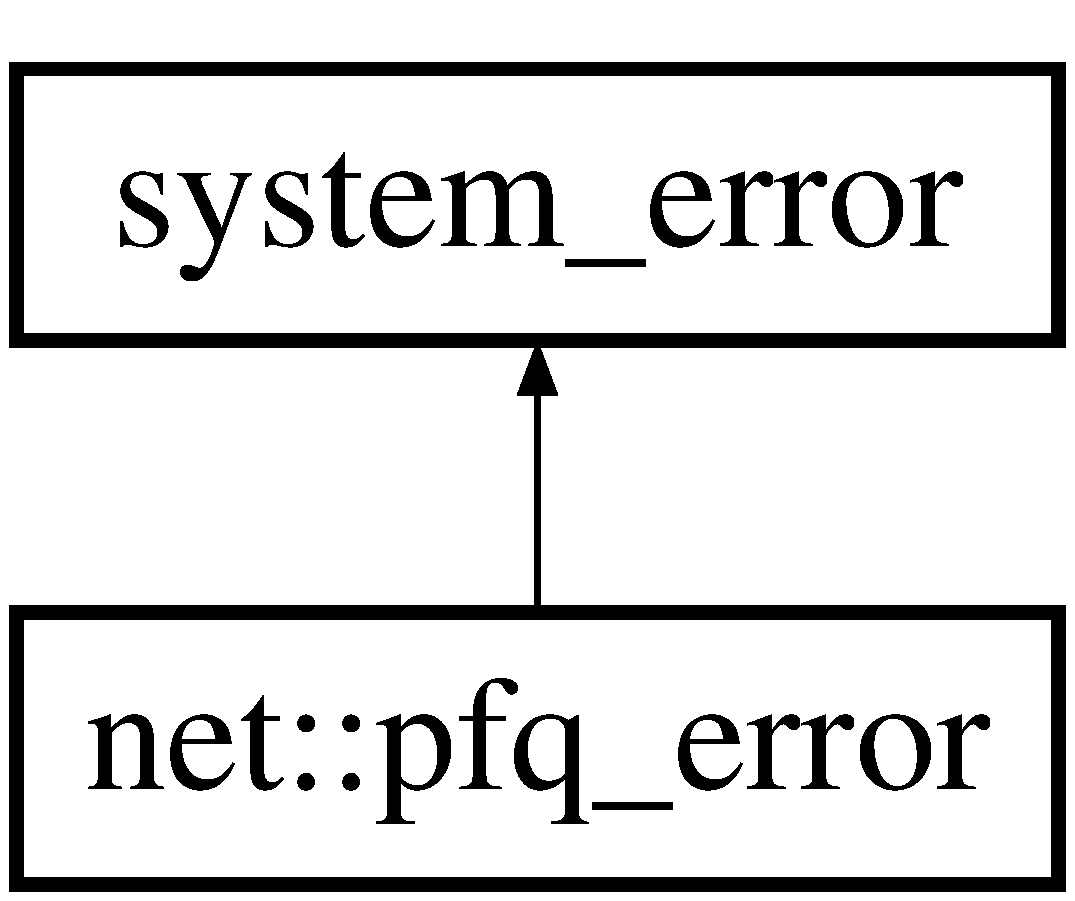
\includegraphics[height=2.000000cm]{classnet_1_1pfq__error}
\end{center}
\end{figure}
\subsection*{Public Member Functions}
\begin{DoxyCompactItemize}
\item 
\hyperlink{classnet_1_1pfq__error_af2d9de405f6302a2b086d124cebefd82}{pfq\-\_\-error} (int ev, const char $\ast$reason)
\item 
\hyperlink{classnet_1_1pfq__error_aad416b1835ae059b8907a1c94e695a2c}{pfq\-\_\-error} (const char $\ast$reason)
\item 
virtual \hyperlink{classnet_1_1pfq__error_abc9c3391a06f55507153b6acbb896eef}{$\sim$pfq\-\_\-error} () noexcept
\end{DoxyCompactItemize}


\subsection{Detailed Description}
Subclass of std\-::system\-\_\-error. 

\hyperlink{classnet_1_1pfq__error}{pfq\-\_\-error} represent problems related to the P\-F\-Q system. 

\subsection{Constructor \& Destructor Documentation}
\hypertarget{classnet_1_1pfq__error_af2d9de405f6302a2b086d124cebefd82}{\index{net\-::pfq\-\_\-error@{net\-::pfq\-\_\-error}!pfq\-\_\-error@{pfq\-\_\-error}}
\index{pfq\-\_\-error@{pfq\-\_\-error}!net::pfq_error@{net\-::pfq\-\_\-error}}
\subsubsection[{pfq\-\_\-error}]{\setlength{\rightskip}{0pt plus 5cm}net\-::pfq\-\_\-error\-::pfq\-\_\-error (
\begin{DoxyParamCaption}
\item[{int}]{ev, }
\item[{const char $\ast$}]{reason}
\end{DoxyParamCaption}
)\hspace{0.3cm}{\ttfamily [inline]}}}\label{classnet_1_1pfq__error_af2d9de405f6302a2b086d124cebefd82}
\hypertarget{classnet_1_1pfq__error_aad416b1835ae059b8907a1c94e695a2c}{\index{net\-::pfq\-\_\-error@{net\-::pfq\-\_\-error}!pfq\-\_\-error@{pfq\-\_\-error}}
\index{pfq\-\_\-error@{pfq\-\_\-error}!net::pfq_error@{net\-::pfq\-\_\-error}}
\subsubsection[{pfq\-\_\-error}]{\setlength{\rightskip}{0pt plus 5cm}net\-::pfq\-\_\-error\-::pfq\-\_\-error (
\begin{DoxyParamCaption}
\item[{const char $\ast$}]{reason}
\end{DoxyParamCaption}
)\hspace{0.3cm}{\ttfamily [inline]}}}\label{classnet_1_1pfq__error_aad416b1835ae059b8907a1c94e695a2c}
\hypertarget{classnet_1_1pfq__error_abc9c3391a06f55507153b6acbb896eef}{\index{net\-::pfq\-\_\-error@{net\-::pfq\-\_\-error}!$\sim$pfq\-\_\-error@{$\sim$pfq\-\_\-error}}
\index{$\sim$pfq\-\_\-error@{$\sim$pfq\-\_\-error}!net::pfq_error@{net\-::pfq\-\_\-error}}
\subsubsection[{$\sim$pfq\-\_\-error}]{\setlength{\rightskip}{0pt plus 5cm}virtual net\-::pfq\-\_\-error\-::$\sim$pfq\-\_\-error (
\begin{DoxyParamCaption}
{}
\end{DoxyParamCaption}
)\hspace{0.3cm}{\ttfamily [inline]}, {\ttfamily [virtual]}, {\ttfamily [noexcept]}}}\label{classnet_1_1pfq__error_abc9c3391a06f55507153b6acbb896eef}


The documentation for this class was generated from the following file\-:\begin{DoxyCompactItemize}
\item 
/root/\-Git\-Hub/\-P\-F\-Q/user/\-C++/\hyperlink{pfq-except_8hpp}{pfq-\/except.\-hpp}\end{DoxyCompactItemize}

\hypertarget{structnet_1_1param_1_1policy}{\section{net\-:\-:param\-:\-:policy Struct Reference}
\label{structnet_1_1param_1_1policy}\index{net\-::param\-::policy@{net\-::param\-::policy}}
}


{\ttfamily \#include $<$pfq.\-hpp$>$}

\subsection*{Public Attributes}
\begin{DoxyCompactItemize}
\item 
\hyperlink{namespacenet_aedc1a0dde937ddbd0800af02920b1067}{group\-\_\-policy} \hyperlink{structnet_1_1param_1_1policy_abc94abaa3c703a34753cd42f435d03f6}{value}
\end{DoxyCompactItemize}


\subsection{Member Data Documentation}
\hypertarget{structnet_1_1param_1_1policy_abc94abaa3c703a34753cd42f435d03f6}{\index{net\-::param\-::policy@{net\-::param\-::policy}!value@{value}}
\index{value@{value}!net::param::policy@{net\-::param\-::policy}}
\subsubsection[{value}]{\setlength{\rightskip}{0pt plus 5cm}{\bf group\-\_\-policy} net\-::param\-::policy\-::value}}\label{structnet_1_1param_1_1policy_abc94abaa3c703a34753cd42f435d03f6}


The documentation for this struct was generated from the following file\-:\begin{DoxyCompactItemize}
\item 
/root/\-Git\-Hub/\-P\-F\-Q/user/\-C++/\hyperlink{pfq_8hpp}{pfq.\-hpp}\end{DoxyCompactItemize}

\hypertarget{classnet_1_1queue}{\section{net\-:\-:queue Class Reference}
\label{classnet_1_1queue}\index{net\-::queue@{net\-::queue}}
}


This class represent a queue of packets.  




{\ttfamily \#include $<$pfq-\/queue.\-hpp$>$}

\subsection*{Classes}
\begin{DoxyCompactItemize}
\item 
struct \hyperlink{structnet_1_1queue_1_1const__iterator}{const\-\_\-iterator}
\begin{DoxyCompactList}\small\item\em Constant forward iterator over packets. \end{DoxyCompactList}\item 
struct \hyperlink{structnet_1_1queue_1_1iterator}{iterator}
\begin{DoxyCompactList}\small\item\em Forward iterator over packets. \end{DoxyCompactList}\end{DoxyCompactItemize}
\subsection*{Public Member Functions}
\begin{DoxyCompactItemize}
\item 
\hyperlink{classnet_1_1queue_a01a9de73c767d546dcb9a92261043d56}{queue} (void $\ast$addr, size\-\_\-t \hyperlink{classnet_1_1queue_a2c7afc4348eac62342496a735280f265}{slot\-\_\-size}, size\-\_\-t queue\-\_\-len, size\-\_\-t \hyperlink{classnet_1_1queue_a74abf50853b60b5562f12d2294474e59}{index})
\begin{DoxyCompactList}\small\item\em Constructor. \end{DoxyCompactList}\item 
\hyperlink{classnet_1_1queue_acc80b84e74464ee1b86d09f7b600eb54}{$\sim$queue} ()=default
\item 
size\-\_\-t \hyperlink{classnet_1_1queue_a49bbc6d786386012d46b7d2b6b3f2a88}{size} () const 
\begin{DoxyCompactList}\small\item\em Return the number of packets stored in this queue. \end{DoxyCompactList}\item 
bool \hyperlink{classnet_1_1queue_a3ec8373251edb7cdd4be0283ad561a44}{empty} () const 
\begin{DoxyCompactList}\small\item\em Check whether the queue is empty. \end{DoxyCompactList}\item 
size\-\_\-t \hyperlink{classnet_1_1queue_a74abf50853b60b5562f12d2294474e59}{index} () const 
\begin{DoxyCompactList}\small\item\em Return the index position. \end{DoxyCompactList}\item 
size\-\_\-t \hyperlink{classnet_1_1queue_a2c7afc4348eac62342496a735280f265}{slot\-\_\-size} () const 
\begin{DoxyCompactList}\small\item\em Return the size of the queue slot, in bytes. \end{DoxyCompactList}\item 
const void $\ast$ \hyperlink{classnet_1_1queue_a3c962730a1bfbff1514319f7ca86cbc2}{data} () const 
\begin{DoxyCompactList}\small\item\em Return the pointer to the packet. \end{DoxyCompactList}\item 
\hyperlink{structnet_1_1queue_1_1iterator}{iterator} \hyperlink{classnet_1_1queue_afe83b7428a3a78ba133c7ca2b568b67a}{begin} ()
\begin{DoxyCompactList}\small\item\em Return an iterator to the first slot of a non-\/empty queue. \end{DoxyCompactList}\item 
\hyperlink{structnet_1_1queue_1_1const__iterator}{const\-\_\-iterator} \hyperlink{classnet_1_1queue_a2babffc7f46dc271a8b2234970ca9b79}{begin} () const 
\begin{DoxyCompactList}\small\item\em Return a constant iterator to the first slot of a non-\/empty queue. \end{DoxyCompactList}\item 
\hyperlink{structnet_1_1queue_1_1iterator}{iterator} \hyperlink{classnet_1_1queue_ab18b037cd983bdbbc8eeb92b7cff12ce}{end} ()
\begin{DoxyCompactList}\small\item\em Return an iterator past to the end of the queue. \end{DoxyCompactList}\item 
\hyperlink{structnet_1_1queue_1_1const__iterator}{const\-\_\-iterator} \hyperlink{classnet_1_1queue_ad7d4205997d94ae5ff6e7997ea63976d}{end} () const 
\begin{DoxyCompactList}\small\item\em Return a constant iterator past to the end of the queue. \end{DoxyCompactList}\item 
\hyperlink{structnet_1_1queue_1_1const__iterator}{const\-\_\-iterator} \hyperlink{classnet_1_1queue_a7590f2c5b9b48b1ea44104a1bab6d21d}{cbegin} () const 
\begin{DoxyCompactList}\small\item\em Return a constant iterator to the first slot of an non-\/empty queue. \end{DoxyCompactList}\item 
\hyperlink{structnet_1_1queue_1_1const__iterator}{const\-\_\-iterator} \hyperlink{classnet_1_1queue_a17d5c7e685e6bba36e361a2a4fafeedb}{cend} () const 
\begin{DoxyCompactList}\small\item\em Return a constant iterator past to the end of the queue. \end{DoxyCompactList}\end{DoxyCompactItemize}


\subsection{Detailed Description}
This class represent a queue of packets. 

The memory where packets are stored is not owned by this class. 

\subsection{Constructor \& Destructor Documentation}
\hypertarget{classnet_1_1queue_a01a9de73c767d546dcb9a92261043d56}{\index{net\-::queue@{net\-::queue}!queue@{queue}}
\index{queue@{queue}!net::queue@{net\-::queue}}
\subsubsection[{queue}]{\setlength{\rightskip}{0pt plus 5cm}net\-::queue\-::queue (
\begin{DoxyParamCaption}
\item[{void $\ast$}]{addr, }
\item[{size\-\_\-t}]{slot\-\_\-size, }
\item[{size\-\_\-t}]{queue\-\_\-len, }
\item[{size\-\_\-t}]{index}
\end{DoxyParamCaption}
)\hspace{0.3cm}{\ttfamily [inline]}}}\label{classnet_1_1queue_a01a9de73c767d546dcb9a92261043d56}


Constructor. 

Construct a queue descriptor, stored at the given address. \hypertarget{classnet_1_1queue_acc80b84e74464ee1b86d09f7b600eb54}{\index{net\-::queue@{net\-::queue}!$\sim$queue@{$\sim$queue}}
\index{$\sim$queue@{$\sim$queue}!net::queue@{net\-::queue}}
\subsubsection[{$\sim$queue}]{\setlength{\rightskip}{0pt plus 5cm}net\-::queue\-::$\sim$queue (
\begin{DoxyParamCaption}
{}
\end{DoxyParamCaption}
)\hspace{0.3cm}{\ttfamily [default]}}}\label{classnet_1_1queue_acc80b84e74464ee1b86d09f7b600eb54}


\subsection{Member Function Documentation}
\hypertarget{classnet_1_1queue_afe83b7428a3a78ba133c7ca2b568b67a}{\index{net\-::queue@{net\-::queue}!begin@{begin}}
\index{begin@{begin}!net::queue@{net\-::queue}}
\subsubsection[{begin}]{\setlength{\rightskip}{0pt plus 5cm}{\bf iterator} net\-::queue\-::begin (
\begin{DoxyParamCaption}
{}
\end{DoxyParamCaption}
)\hspace{0.3cm}{\ttfamily [inline]}}}\label{classnet_1_1queue_afe83b7428a3a78ba133c7ca2b568b67a}


Return an iterator to the first slot of a non-\/empty queue. 

Return \hyperlink{classnet_1_1queue_ab18b037cd983bdbbc8eeb92b7cff12ce}{end()} in case of empty queue. \hypertarget{classnet_1_1queue_a2babffc7f46dc271a8b2234970ca9b79}{\index{net\-::queue@{net\-::queue}!begin@{begin}}
\index{begin@{begin}!net::queue@{net\-::queue}}
\subsubsection[{begin}]{\setlength{\rightskip}{0pt plus 5cm}{\bf const\-\_\-iterator} net\-::queue\-::begin (
\begin{DoxyParamCaption}
{}
\end{DoxyParamCaption}
) const\hspace{0.3cm}{\ttfamily [inline]}}}\label{classnet_1_1queue_a2babffc7f46dc271a8b2234970ca9b79}


Return a constant iterator to the first slot of a non-\/empty queue. 

Return \hyperlink{classnet_1_1queue_ab18b037cd983bdbbc8eeb92b7cff12ce}{end()} in case of empty queue. \hypertarget{classnet_1_1queue_a7590f2c5b9b48b1ea44104a1bab6d21d}{\index{net\-::queue@{net\-::queue}!cbegin@{cbegin}}
\index{cbegin@{cbegin}!net::queue@{net\-::queue}}
\subsubsection[{cbegin}]{\setlength{\rightskip}{0pt plus 5cm}{\bf const\-\_\-iterator} net\-::queue\-::cbegin (
\begin{DoxyParamCaption}
{}
\end{DoxyParamCaption}
) const\hspace{0.3cm}{\ttfamily [inline]}}}\label{classnet_1_1queue_a7590f2c5b9b48b1ea44104a1bab6d21d}


Return a constant iterator to the first slot of an non-\/empty queue. 

Return \hyperlink{classnet_1_1queue_a17d5c7e685e6bba36e361a2a4fafeedb}{cend()} in case of empty queue. \hypertarget{classnet_1_1queue_a17d5c7e685e6bba36e361a2a4fafeedb}{\index{net\-::queue@{net\-::queue}!cend@{cend}}
\index{cend@{cend}!net::queue@{net\-::queue}}
\subsubsection[{cend}]{\setlength{\rightskip}{0pt plus 5cm}{\bf const\-\_\-iterator} net\-::queue\-::cend (
\begin{DoxyParamCaption}
{}
\end{DoxyParamCaption}
) const\hspace{0.3cm}{\ttfamily [inline]}}}\label{classnet_1_1queue_a17d5c7e685e6bba36e361a2a4fafeedb}


Return a constant iterator past to the end of the queue. 

\hypertarget{classnet_1_1queue_a3c962730a1bfbff1514319f7ca86cbc2}{\index{net\-::queue@{net\-::queue}!data@{data}}
\index{data@{data}!net::queue@{net\-::queue}}
\subsubsection[{data}]{\setlength{\rightskip}{0pt plus 5cm}const void$\ast$ net\-::queue\-::data (
\begin{DoxyParamCaption}
{}
\end{DoxyParamCaption}
) const\hspace{0.3cm}{\ttfamily [inline]}}}\label{classnet_1_1queue_a3c962730a1bfbff1514319f7ca86cbc2}


Return the pointer to the packet. 

\hypertarget{classnet_1_1queue_a3ec8373251edb7cdd4be0283ad561a44}{\index{net\-::queue@{net\-::queue}!empty@{empty}}
\index{empty@{empty}!net::queue@{net\-::queue}}
\subsubsection[{empty}]{\setlength{\rightskip}{0pt plus 5cm}bool net\-::queue\-::empty (
\begin{DoxyParamCaption}
{}
\end{DoxyParamCaption}
) const\hspace{0.3cm}{\ttfamily [inline]}}}\label{classnet_1_1queue_a3ec8373251edb7cdd4be0283ad561a44}


Check whether the queue is empty. 

\hypertarget{classnet_1_1queue_ab18b037cd983bdbbc8eeb92b7cff12ce}{\index{net\-::queue@{net\-::queue}!end@{end}}
\index{end@{end}!net::queue@{net\-::queue}}
\subsubsection[{end}]{\setlength{\rightskip}{0pt plus 5cm}{\bf iterator} net\-::queue\-::end (
\begin{DoxyParamCaption}
{}
\end{DoxyParamCaption}
)\hspace{0.3cm}{\ttfamily [inline]}}}\label{classnet_1_1queue_ab18b037cd983bdbbc8eeb92b7cff12ce}


Return an iterator past to the end of the queue. 

\hypertarget{classnet_1_1queue_ad7d4205997d94ae5ff6e7997ea63976d}{\index{net\-::queue@{net\-::queue}!end@{end}}
\index{end@{end}!net::queue@{net\-::queue}}
\subsubsection[{end}]{\setlength{\rightskip}{0pt plus 5cm}{\bf const\-\_\-iterator} net\-::queue\-::end (
\begin{DoxyParamCaption}
{}
\end{DoxyParamCaption}
) const\hspace{0.3cm}{\ttfamily [inline]}}}\label{classnet_1_1queue_ad7d4205997d94ae5ff6e7997ea63976d}


Return a constant iterator past to the end of the queue. 

\hypertarget{classnet_1_1queue_a74abf50853b60b5562f12d2294474e59}{\index{net\-::queue@{net\-::queue}!index@{index}}
\index{index@{index}!net::queue@{net\-::queue}}
\subsubsection[{index}]{\setlength{\rightskip}{0pt plus 5cm}size\-\_\-t net\-::queue\-::index (
\begin{DoxyParamCaption}
{}
\end{DoxyParamCaption}
) const\hspace{0.3cm}{\ttfamily [inline]}}}\label{classnet_1_1queue_a74abf50853b60b5562f12d2294474e59}


Return the index position. 

\hypertarget{classnet_1_1queue_a49bbc6d786386012d46b7d2b6b3f2a88}{\index{net\-::queue@{net\-::queue}!size@{size}}
\index{size@{size}!net::queue@{net\-::queue}}
\subsubsection[{size}]{\setlength{\rightskip}{0pt plus 5cm}size\-\_\-t net\-::queue\-::size (
\begin{DoxyParamCaption}
{}
\end{DoxyParamCaption}
) const\hspace{0.3cm}{\ttfamily [inline]}}}\label{classnet_1_1queue_a49bbc6d786386012d46b7d2b6b3f2a88}


Return the number of packets stored in this queue. 

\hypertarget{classnet_1_1queue_a2c7afc4348eac62342496a735280f265}{\index{net\-::queue@{net\-::queue}!slot\-\_\-size@{slot\-\_\-size}}
\index{slot\-\_\-size@{slot\-\_\-size}!net::queue@{net\-::queue}}
\subsubsection[{slot\-\_\-size}]{\setlength{\rightskip}{0pt plus 5cm}size\-\_\-t net\-::queue\-::slot\-\_\-size (
\begin{DoxyParamCaption}
{}
\end{DoxyParamCaption}
) const\hspace{0.3cm}{\ttfamily [inline]}}}\label{classnet_1_1queue_a2c7afc4348eac62342496a735280f265}


Return the size of the queue slot, in bytes. 



The documentation for this class was generated from the following file\-:\begin{DoxyCompactItemize}
\item 
/root/\-Git\-Hub/\-P\-F\-Q/user/\-C++/\hyperlink{pfq-queue_8hpp}{pfq-\/queue.\-hpp}\end{DoxyCompactItemize}

\hypertarget{structnet_1_1param_1_1rx__slots}{\section{net\+:\+:param\+:\+:rx\+\_\+slots Struct Reference}
\label{structnet_1_1param_1_1rx__slots}\index{net\+::param\+::rx\+\_\+slots@{net\+::param\+::rx\+\_\+slots}}
}


{\ttfamily \#include $<$pfq.\+hpp$>$}

\subsection*{Public Attributes}
\begin{DoxyCompactItemize}
\item 
size\+\_\+t \hyperlink{structnet_1_1param_1_1rx__slots_a7faa81257d9e7f5d55d33e5893f238b8}{value}
\end{DoxyCompactItemize}


\subsection{Member Data Documentation}
\hypertarget{structnet_1_1param_1_1rx__slots_a7faa81257d9e7f5d55d33e5893f238b8}{\index{net\+::param\+::rx\+\_\+slots@{net\+::param\+::rx\+\_\+slots}!value@{value}}
\index{value@{value}!net\+::param\+::rx\+\_\+slots@{net\+::param\+::rx\+\_\+slots}}
\subsubsection[{value}]{\setlength{\rightskip}{0pt plus 5cm}size\+\_\+t net\+::param\+::rx\+\_\+slots\+::value}}\label{structnet_1_1param_1_1rx__slots_a7faa81257d9e7f5d55d33e5893f238b8}


The documentation for this struct was generated from the following file\+:\begin{DoxyCompactItemize}
\item 
C++/\hyperlink{pfq_8hpp}{pfq.\+hpp}\end{DoxyCompactItemize}

\hypertarget{structnet_1_1param_1_1tx__slots}{\section{net\-:\-:param\-:\-:tx\-\_\-slots Struct Reference}
\label{structnet_1_1param_1_1tx__slots}\index{net\-::param\-::tx\-\_\-slots@{net\-::param\-::tx\-\_\-slots}}
}


{\ttfamily \#include $<$pfq.\-hpp$>$}

\subsection*{Public Attributes}
\begin{DoxyCompactItemize}
\item 
size\-\_\-t \hyperlink{structnet_1_1param_1_1tx__slots_aa9c38079016460b21e406579485f94a1}{value}
\end{DoxyCompactItemize}


\subsection{Member Data Documentation}
\hypertarget{structnet_1_1param_1_1tx__slots_aa9c38079016460b21e406579485f94a1}{\index{net\-::param\-::tx\-\_\-slots@{net\-::param\-::tx\-\_\-slots}!value@{value}}
\index{value@{value}!net::param::tx_slots@{net\-::param\-::tx\-\_\-slots}}
\subsubsection[{value}]{\setlength{\rightskip}{0pt plus 5cm}size\-\_\-t net\-::param\-::tx\-\_\-slots\-::value}}\label{structnet_1_1param_1_1tx__slots_aa9c38079016460b21e406579485f94a1}


The documentation for this struct was generated from the following file\-:\begin{DoxyCompactItemize}
\item 
/root/\-Git\-Hub/\-P\-F\-Q/user/\-C++/\hyperlink{pfq_8hpp}{pfq.\-hpp}\end{DoxyCompactItemize}

\hypertarget{structnet_1_1param_1_1details_1_1type__index}{\section{net\+:\+:param\+:\+:details\+:\+:type\+\_\+index$<$ Ts $>$ Struct Template Reference}
\label{structnet_1_1param_1_1details_1_1type__index}\index{net\+::param\+::details\+::type\+\_\+index$<$ Ts $>$@{net\+::param\+::details\+::type\+\_\+index$<$ Ts $>$}}
}


{\ttfamily \#include $<$pfq-\/util.\+hpp$>$}



The documentation for this struct was generated from the following file\+:\begin{DoxyCompactItemize}
\item 
C++/\hyperlink{pfq-util_8hpp}{pfq-\/util.\+hpp}\end{DoxyCompactItemize}

\hypertarget{structnet_1_1param_1_1details_1_1type__index_3_01T_00_01T_00_01Ts_8_8_8_4}{\section{net\+:\+:param\+:\+:details\+:\+:type\+\_\+index$<$ T, T, Ts...$>$ Struct Template Reference}
\label{structnet_1_1param_1_1details_1_1type__index_3_01T_00_01T_00_01Ts_8_8_8_4}\index{net\+::param\+::details\+::type\+\_\+index$<$ T, T, Ts...$>$@{net\+::param\+::details\+::type\+\_\+index$<$ T, T, Ts...$>$}}
}


{\ttfamily \#include $<$pfq-\/util.\+hpp$>$}

\subsection*{Public Types}
\begin{DoxyCompactItemize}
\item 
enum \{ \hyperlink{structnet_1_1param_1_1details_1_1type__index_3_01T_00_01T_00_01Ts_8_8_8_4_a040ee215ab90caaa7c12ce856e2d2b2eac990fbaa04445effd47d0e46691f994e}{value} = 0
 \}
\end{DoxyCompactItemize}


\subsection{Member Enumeration Documentation}
\hypertarget{structnet_1_1param_1_1details_1_1type__index_3_01T_00_01T_00_01Ts_8_8_8_4_a040ee215ab90caaa7c12ce856e2d2b2e}{\subsubsection[{anonymous enum}]{\setlength{\rightskip}{0pt plus 5cm}template$<$typename T , typename... Ts$>$ anonymous enum}}\label{structnet_1_1param_1_1details_1_1type__index_3_01T_00_01T_00_01Ts_8_8_8_4_a040ee215ab90caaa7c12ce856e2d2b2e}
\begin{Desc}
\item[Enumerator]\par
\begin{description}
\index{value@{value}!net\+::param\+::details\+::type\+\_\+index$<$ T, T, Ts...$>$@{net\+::param\+::details\+::type\+\_\+index$<$ T, T, Ts...$>$}}\index{net\+::param\+::details\+::type\+\_\+index$<$ T, T, Ts...$>$@{net\+::param\+::details\+::type\+\_\+index$<$ T, T, Ts...$>$}!value@{value}}\item[{\em 
\hypertarget{structnet_1_1param_1_1details_1_1type__index_3_01T_00_01T_00_01Ts_8_8_8_4_a040ee215ab90caaa7c12ce856e2d2b2eac990fbaa04445effd47d0e46691f994e}{value}\label{structnet_1_1param_1_1details_1_1type__index_3_01T_00_01T_00_01Ts_8_8_8_4_a040ee215ab90caaa7c12ce856e2d2b2eac990fbaa04445effd47d0e46691f994e}
}]\end{description}
\end{Desc}


The documentation for this struct was generated from the following file\+:\begin{DoxyCompactItemize}
\item 
C++/\hyperlink{pfq-util_8hpp}{pfq-\/util.\+hpp}\end{DoxyCompactItemize}

\hypertarget{structnet_1_1param_1_1details_1_1type__index_3_01T_00_01T0_00_01Ts_8_8_8_4}{\section{net\+:\+:param\+:\+:details\+:\+:type\+\_\+index$<$ T, T0, Ts...$>$ Struct Template Reference}
\label{structnet_1_1param_1_1details_1_1type__index_3_01T_00_01T0_00_01Ts_8_8_8_4}\index{net\+::param\+::details\+::type\+\_\+index$<$ T, T0, Ts...$>$@{net\+::param\+::details\+::type\+\_\+index$<$ T, T0, Ts...$>$}}
}


{\ttfamily \#include $<$pfq-\/util.\+hpp$>$}

\subsection*{Public Types}
\begin{DoxyCompactItemize}
\item 
enum \{ \hyperlink{structnet_1_1param_1_1details_1_1type__index_3_01T_00_01T0_00_01Ts_8_8_8_4_a0e1958d65adb96b5b73afd41372b1a8fac571d4fccf6873682c31e1fa9dd70e56}{value} = 1 + type\+\_\+index$<$T, Ts...$>$\+:\+:value
 \}
\end{DoxyCompactItemize}


\subsection{Member Enumeration Documentation}
\hypertarget{structnet_1_1param_1_1details_1_1type__index_3_01T_00_01T0_00_01Ts_8_8_8_4_a0e1958d65adb96b5b73afd41372b1a8f}{\subsubsection[{anonymous enum}]{\setlength{\rightskip}{0pt plus 5cm}template$<$typename T , typename T0 , typename... Ts$>$ anonymous enum}}\label{structnet_1_1param_1_1details_1_1type__index_3_01T_00_01T0_00_01Ts_8_8_8_4_a0e1958d65adb96b5b73afd41372b1a8f}
\begin{Desc}
\item[Enumerator]\par
\begin{description}
\index{value@{value}!net\+::param\+::details\+::type\+\_\+index$<$ T, T0, Ts...$>$@{net\+::param\+::details\+::type\+\_\+index$<$ T, T0, Ts...$>$}}\index{net\+::param\+::details\+::type\+\_\+index$<$ T, T0, Ts...$>$@{net\+::param\+::details\+::type\+\_\+index$<$ T, T0, Ts...$>$}!value@{value}}\item[{\em 
\hypertarget{structnet_1_1param_1_1details_1_1type__index_3_01T_00_01T0_00_01Ts_8_8_8_4_a0e1958d65adb96b5b73afd41372b1a8fac571d4fccf6873682c31e1fa9dd70e56}{value}\label{structnet_1_1param_1_1details_1_1type__index_3_01T_00_01T0_00_01Ts_8_8_8_4_a0e1958d65adb96b5b73afd41372b1a8fac571d4fccf6873682c31e1fa9dd70e56}
}]\end{description}
\end{Desc}


The documentation for this struct was generated from the following file\+:\begin{DoxyCompactItemize}
\item 
C++/\hyperlink{pfq-util_8hpp}{pfq-\/util.\+hpp}\end{DoxyCompactItemize}

\hypertarget{structnet_1_1param_1_1details_1_1type__index_3_01Tp_01_4}{\section{net\-:\-:param\-:\-:details\-:\-:type\-\_\-index$<$ Tp $>$ Struct Template Reference}
\label{structnet_1_1param_1_1details_1_1type__index_3_01Tp_01_4}\index{net\-::param\-::details\-::type\-\_\-index$<$ Tp $>$@{net\-::param\-::details\-::type\-\_\-index$<$ Tp $>$}}
}


{\ttfamily \#include $<$pfq-\/util.\-hpp$>$}

\subsection*{Public Types}
\begin{DoxyCompactItemize}
\item 
enum \{ \hyperlink{structnet_1_1param_1_1details_1_1type__index_3_01Tp_01_4_aff936ccbc5e8aac0a2398fabfb58cb55a46105c210f804e7866c782cdd2f1c8c9}{value} = 1
 \}
\end{DoxyCompactItemize}


\subsection{Member Enumeration Documentation}
\hypertarget{structnet_1_1param_1_1details_1_1type__index_3_01Tp_01_4_aff936ccbc5e8aac0a2398fabfb58cb55}{\subsubsection[{anonymous enum}]{\setlength{\rightskip}{0pt plus 5cm}template$<$typename Tp $>$ anonymous enum}}\label{structnet_1_1param_1_1details_1_1type__index_3_01Tp_01_4_aff936ccbc5e8aac0a2398fabfb58cb55}
\begin{Desc}
\item[Enumerator]\par
\begin{description}
\index{value@{value}!net\-::param\-::details\-::type\-\_\-index$<$ Tp $>$@{net\-::param\-::details\-::type\-\_\-index$<$ Tp $>$}}\index{net\-::param\-::details\-::type\-\_\-index$<$ Tp $>$@{net\-::param\-::details\-::type\-\_\-index$<$ Tp $>$}!value@{value}}\item[{\em 
\hypertarget{structnet_1_1param_1_1details_1_1type__index_3_01Tp_01_4_aff936ccbc5e8aac0a2398fabfb58cb55a46105c210f804e7866c782cdd2f1c8c9}{value}\label{structnet_1_1param_1_1details_1_1type__index_3_01Tp_01_4_aff936ccbc5e8aac0a2398fabfb58cb55a46105c210f804e7866c782cdd2f1c8c9}
}]\end{description}
\end{Desc}


The documentation for this struct was generated from the following file\-:\begin{DoxyCompactItemize}
\item 
/root/\-Git\-Hub/\-P\-F\-Q/user/\-C++/\hyperlink{pfq-util_8hpp}{pfq-\/util.\-hpp}\end{DoxyCompactItemize}

\hypertarget{structnet_1_1vlan__id}{\section{net\+:\+:vlan\+\_\+id Struct Reference}
\label{structnet_1_1vlan__id}\index{net\+::vlan\+\_\+id@{net\+::vlan\+\_\+id}}
}


vlan options.  




{\ttfamily \#include $<$pfq.\+hpp$>$}

\subsection*{Static Public Attributes}
\begin{DoxyCompactItemize}
\item 
static constexpr int \hyperlink{structnet_1_1vlan__id_a266d270ff167bffcc68b5baf3fa1254f}{untag} = Q\+\_\+\+V\+L\+A\+N\+\_\+\+U\+N\+T\+A\+G
\item 
static constexpr int \hyperlink{structnet_1_1vlan__id_a020dfecb6821c57a45437f534256d712}{anytag} = Q\+\_\+\+V\+L\+A\+N\+\_\+\+A\+N\+Y\+T\+A\+G
\end{DoxyCompactItemize}


\subsection{Detailed Description}
vlan options. 

Special vlan ids are untag (matches with untagged vlans) and anytag. 

\subsection{Member Data Documentation}
\hypertarget{structnet_1_1vlan__id_a020dfecb6821c57a45437f534256d712}{\index{net\+::vlan\+\_\+id@{net\+::vlan\+\_\+id}!anytag@{anytag}}
\index{anytag@{anytag}!net\+::vlan\+\_\+id@{net\+::vlan\+\_\+id}}
\subsubsection[{anytag}]{\setlength{\rightskip}{0pt plus 5cm}constexpr int net\+::vlan\+\_\+id\+::anytag = Q\+\_\+\+V\+L\+A\+N\+\_\+\+A\+N\+Y\+T\+A\+G\hspace{0.3cm}{\ttfamily [static]}}}\label{structnet_1_1vlan__id_a020dfecb6821c57a45437f534256d712}
\hypertarget{structnet_1_1vlan__id_a266d270ff167bffcc68b5baf3fa1254f}{\index{net\+::vlan\+\_\+id@{net\+::vlan\+\_\+id}!untag@{untag}}
\index{untag@{untag}!net\+::vlan\+\_\+id@{net\+::vlan\+\_\+id}}
\subsubsection[{untag}]{\setlength{\rightskip}{0pt plus 5cm}constexpr int net\+::vlan\+\_\+id\+::untag = Q\+\_\+\+V\+L\+A\+N\+\_\+\+U\+N\+T\+A\+G\hspace{0.3cm}{\ttfamily [static]}}}\label{structnet_1_1vlan__id_a266d270ff167bffcc68b5baf3fa1254f}


The documentation for this struct was generated from the following file\+:\begin{DoxyCompactItemize}
\item 
C++/\hyperlink{pfq_8hpp}{pfq.\+hpp}\end{DoxyCompactItemize}

\chapter{File Documentation}
\hypertarget{pfq-except_8hpp}{\section{/root/\-Git\-Hub/\-P\-F\-Q/user/\-C++/pfq-\/except.hpp File Reference}
\label{pfq-except_8hpp}\index{/root/\-Git\-Hub/\-P\-F\-Q/user/\-C++/pfq-\/except.\-hpp@{/root/\-Git\-Hub/\-P\-F\-Q/user/\-C++/pfq-\/except.\-hpp}}
}
{\ttfamily \#include $<$system\-\_\-error$>$}\\*
\subsection*{Classes}
\begin{DoxyCompactItemize}
\item 
class \hyperlink{classnet_1_1pfq__error}{net\-::pfq\-\_\-error}
\begin{DoxyCompactList}\small\item\em Subclass of std\-::system\-\_\-error. \end{DoxyCompactList}\end{DoxyCompactItemize}
\subsection*{Namespaces}
\begin{DoxyCompactItemize}
\item 
\hyperlink{namespacenet}{net}
\end{DoxyCompactItemize}

\hypertarget{pfq-queue_8hpp}{\section{C++/pfq-\/queue.hpp File Reference}
\label{pfq-queue_8hpp}\index{C++/pfq-\/queue.\-hpp@{C++/pfq-\/queue.\-hpp}}
}
{\ttfamily \#include $<$iterator$>$}\\*
{\ttfamily \#include $<$linux/pf\-\_\-q.\-h$>$}\\*
\subsection*{Classes}
\begin{DoxyCompactItemize}
\item 
class \hyperlink{classnet_1_1queue}{net\-::queue}
\begin{DoxyCompactList}\small\item\em This class represent a queue of packets. \end{DoxyCompactList}\item 
struct \hyperlink{structnet_1_1queue_1_1iterator}{net\-::queue\-::iterator}
\begin{DoxyCompactList}\small\item\em Forward iterator over packets. \end{DoxyCompactList}\item 
struct \hyperlink{structnet_1_1queue_1_1const__iterator}{net\-::queue\-::const\-\_\-iterator}
\begin{DoxyCompactList}\small\item\em Constant forward iterator over packets. \end{DoxyCompactList}\end{DoxyCompactItemize}
\subsection*{Namespaces}
\begin{DoxyCompactItemize}
\item 
\hyperlink{namespacenet}{net}
\end{DoxyCompactItemize}

\hypertarget{pfq-util_8hpp}{\section{C++/pfq-\/util.hpp File Reference}
\label{pfq-util_8hpp}\index{C++/pfq-\/util.\+hpp@{C++/pfq-\/util.\+hpp}}
}
{\ttfamily \#include $<$vector$>$}\\*
{\ttfamily \#include $<$tuple$>$}\\*
{\ttfamily \#include $<$string$>$}\\*
{\ttfamily \#include $<$cstring$>$}\\*
{\ttfamily \#include $<$stdexcept$>$}\\*
{\ttfamily \#include $<$system\+\_\+error$>$}\\*
{\ttfamily \#include $<$fstream$>$}\\*
{\ttfamily \#include $<$iterator$>$}\\*
{\ttfamily \#include $<$thread$>$}\\*
{\ttfamily \#include $<$algorithm$>$}\\*
{\ttfamily \#include $<$linux/pf\+\_\+q.\+h$>$}\\*
{\ttfamily \#include $<$sys/ioctl.\+h$>$}\\*
{\ttfamily \#include $<$net/if.\+h$>$}\\*
{\ttfamily \#include $<$pfq-\/except.\+hpp$>$}\\*
\subsection*{Classes}
\begin{DoxyCompactItemize}
\item 
struct \hyperlink{structpfq_1_1param_1_1details_1_1type__index}{pfq\+::param\+::details\+::type\+\_\+index$<$ Ts $>$}
\item 
struct \hyperlink{structpfq_1_1param_1_1details_1_1type__index_3_01T_00_01T_00_01Ts_8_8_8_4}{pfq\+::param\+::details\+::type\+\_\+index$<$ T, T, Ts...$>$}
\item 
struct \hyperlink{structpfq_1_1param_1_1details_1_1type__index_3_01T_00_01T0_00_01Ts_8_8_8_4}{pfq\+::param\+::details\+::type\+\_\+index$<$ T, T0, Ts...$>$}
\item 
struct \hyperlink{structpfq_1_1param_1_1details_1_1type__index_3_01Tp_01_4}{pfq\+::param\+::details\+::type\+\_\+index$<$ Tp $>$}
\end{DoxyCompactItemize}
\subsection*{Namespaces}
\begin{DoxyCompactItemize}
\item 
 \hyperlink{namespacepfq}{pfq}
\item 
 \hyperlink{namespacepfq_1_1param}{pfq\+::param}
\begin{DoxyCompactList}\small\item\em open parameters. \end{DoxyCompactList}\item 
 \hyperlink{namespacepfq_1_1param_1_1details}{pfq\+::param\+::details}
\end{DoxyCompactItemize}
\subsection*{Typedefs}
\begin{DoxyCompactItemize}
\item 
using \hyperlink{namespacepfq_ad7b88920eaf729154354741132483ea8}{pfq\+::mutable\+\_\+buffer} = std\+::pair$<$ char $\ast$, size\+\_\+t $>$
\item 
using \hyperlink{namespacepfq_ac835a1bd09b4cbaba61c100b50d0a99f}{pfq\+::const\+\_\+buffer} = std\+::pair$<$ const char $\ast$, const size\+\_\+t $>$
\end{DoxyCompactItemize}
\subsection*{Functions}
\begin{DoxyCompactItemize}
\item 
{\footnotesize template$<$size\+\_\+t N, typename T $>$ }\\T \hyperlink{namespacepfq_a9db75e7163c5f764248401d10a2a3f9b}{pfq\+::align} (T value)
\begin{DoxyCompactList}\small\item\em Return the value aligned to the next power of two. \end{DoxyCompactList}\item 
int \hyperlink{namespacepfq_a251ac5cc269aa123009754edf62ab8b4}{pfq\+::ifindex} (int fd, const char $\ast$dev)
\begin{DoxyCompactList}\small\item\em Given a device name, return the interface index. \end{DoxyCompactList}\item 
void \hyperlink{namespacepfq_a62b9f1831dc714353f6edcb66a4fad4d}{pfq\+::set\+\_\+promisc} (int fd, const char $\ast$dev, bool value)
\begin{DoxyCompactList}\small\item\em Set/unset the promiscuous mode for the given device. \end{DoxyCompactList}\item 
unsigned int \hyperlink{namespacepfq_a55d90c336462015bb2b4e40f9f853847}{pfq\+::nametoindex} (const char $\ast$dev)
\begin{DoxyCompactList}\small\item\em Given the device name return the related index. \end{DoxyCompactList}\item 
std\+::string \hyperlink{namespacepfq_a7bf753b90ae15e20c86f40ba59c87c36}{pfq\+::indextoname} (unsigned int i)
\begin{DoxyCompactList}\small\item\em Given the index return the related device name. \end{DoxyCompactList}\item 
std\+::string \hyperlink{namespacepfq_a02a1861a64cc518394d3cc4361799c9f}{pfq\+::trim} (std\+::string str)
\begin{DoxyCompactList}\small\item\em Trim pending and trailing whitespaces from a string. \end{DoxyCompactList}\item 
std\+::vector$<$ std\+::string $>$ \hyperlink{namespacepfq_a0c3aeb61dfd544cb08cb240202caf213}{pfq\+::split} (std\+::string str, const char $\ast$sep)
\begin{DoxyCompactList}\small\item\em Split a string by means of the given separator. \end{DoxyCompactList}\item 
unsigned int \hyperlink{namespacepfq_a9a9e9be8b77976ed45483448f54de1f9}{pfq\+::hardware\+\_\+concurrency} ()
\begin{DoxyCompactList}\small\item\em Hardware concurrency. \end{DoxyCompactList}\item 
{\footnotesize template$<$typename T , typename... Ts$>$ }\\auto \hyperlink{namespacepfq_1_1param_a09da2abc1a228d7f77c35bed3bdb157d}{pfq\+::param\+::get} (std\+::tuple$<$ Ts...$>$ \&tup) -\/$>$ decltype(std\+::get$<$ details\+::type\+\_\+index$<$ T, Ts...$>$\+::value $>$(tup))
\item 
{\footnotesize template$<$typename Tup , typename... Ts$>$ }\\void \hyperlink{namespacepfq_1_1param_aeabbdcec021e01a0a9321678fea99d8f}{pfq\+::param\+::load} (Tup \&tup, Ts \&\&...arg)
\end{DoxyCompactItemize}

\hypertarget{pfq_8hpp}{}\section{C++/pfq/pfq.hpp File Reference}
\label{pfq_8hpp}\index{C++/pfq/pfq.\+hpp@{C++/pfq/pfq.\+hpp}}
{\ttfamily \#include $<$cstddef$>$}\newline
{\ttfamily \#include $<$tuple$>$}\newline
{\ttfamily \#include $<$memory$>$}\newline
{\ttfamily \#include $<$vector$>$}\newline
{\ttfamily \#include $<$type\+\_\+traits$>$}\newline
{\ttfamily \#include $<$algorithm$>$}\newline
{\ttfamily \#include $<$thread$>$}\newline
{\ttfamily \#include $<$chrono$>$}\newline
{\ttfamily \#include $<$pfq/util.\+hpp$>$}\newline
{\ttfamily \#include $<$pfq/queue.\+hpp$>$}\newline
{\ttfamily \#include $<$pfq/lang/lang.\+hpp$>$}\newline
{\ttfamily \#include $<$linux/if\+\_\+ether.\+h$>$}\newline
{\ttfamily \#include $<$linux/ip.\+h$>$}\newline
{\ttfamily \#include $<$linux/pf\+\_\+q.\+h$>$}\newline
{\ttfamily \#include $<$sys/types.\+h$>$}\newline
{\ttfamily \#include $<$sys/stat.\+h$>$}\newline
{\ttfamily \#include $<$sys/socket.\+h$>$}\newline
{\ttfamily \#include $<$sys/ioctl.\+h$>$}\newline
{\ttfamily \#include $<$arpa/inet.\+h$>$}\newline
{\ttfamily \#include $<$net/if.\+h$>$}\newline
{\ttfamily \#include $<$sys/mman.\+h$>$}\newline
{\ttfamily \#include $<$fcntl.\+h$>$}\newline
{\ttfamily \#include $<$poll.\+h$>$}\newline
{\ttfamily \#include $<$pfq/pfq-\/int.\+h$>$}\newline
{\ttfamily \#include $<$pfq/pfq.\+h$>$}\newline
\subsection*{Classes}
\begin{DoxyCompactItemize}
\item 
struct \hyperlink{structpfq_1_1vlan__id}{pfq\+::vlan\+\_\+id}
\begin{DoxyCompactList}\small\item\em vlan options. \end{DoxyCompactList}\item 
struct \hyperlink{structpfq_1_1param_1_1class__}{pfq\+::param\+::class\+\_\+}
\item 
struct \hyperlink{structpfq_1_1param_1_1policy}{pfq\+::param\+::policy}
\item 
struct \hyperlink{structpfq_1_1param_1_1caplen}{pfq\+::param\+::caplen}
\item 
struct \hyperlink{structpfq_1_1param_1_1xmitlen}{pfq\+::param\+::xmitlen}
\item 
struct \hyperlink{structpfq_1_1param_1_1rx__slots}{pfq\+::param\+::rx\+\_\+slots}
\item 
struct \hyperlink{structpfq_1_1param_1_1tx__slots}{pfq\+::param\+::tx\+\_\+slots}
\item 
class \hyperlink{classpfq_1_1socket}{pfq\+::socket}
\begin{DoxyCompactList}\small\item\em P\+FQ\+: the socket. \end{DoxyCompactList}\end{DoxyCompactItemize}
\subsection*{Namespaces}
\begin{DoxyCompactItemize}
\item 
 \hyperlink{namespacepfq}{pfq}
\item 
 \hyperlink{namespacepfq_1_1param}{pfq\+::param}
\begin{DoxyCompactList}\small\item\em open parameters. \end{DoxyCompactList}\end{DoxyCompactItemize}
\subsection*{Typedefs}
\begin{DoxyCompactItemize}
\item 
using \hyperlink{namespacepfq_1_1param_adbf782e10a59b40189d34c425ff8218e}{pfq\+::param\+::types} = std\+::tuple$<$ caplen, xmitlen, rx\+\_\+slots, tx\+\_\+slots, policy, class\+\_\+ $>$
\end{DoxyCompactItemize}
\subsection*{Enumerations}
\begin{DoxyCompactItemize}
\item 
enum \hyperlink{namespacepfq_ac41249c8510558905b01fa4d866a38d7}{pfq\+::group\+\_\+policy} \+: int16\+\_\+t \{ \hyperlink{namespacepfq_ac41249c8510558905b01fa4d866a38d7a5e543256c480ac577d30f76f9120eb74}{pfq\+::group\+\_\+policy\+::undefined} = Q\+\_\+\+P\+O\+L\+I\+C\+Y\+\_\+\+G\+R\+O\+U\+P\+\_\+\+U\+N\+D\+E\+F\+I\+N\+ED, 
\hyperlink{namespacepfq_ac41249c8510558905b01fa4d866a38d7a908b453051b556e053731714a5193921}{pfq\+::group\+\_\+policy\+::priv} = Q\+\_\+\+P\+O\+L\+I\+C\+Y\+\_\+\+G\+R\+O\+U\+P\+\_\+\+P\+R\+I\+V\+A\+TE, 
\hyperlink{namespacepfq_ac41249c8510558905b01fa4d866a38d7ac89b33f8b3f6f452ef6f07d397b5dcdf}{pfq\+::group\+\_\+policy\+::restricted} = Q\+\_\+\+P\+O\+L\+I\+C\+Y\+\_\+\+G\+R\+O\+U\+P\+\_\+\+R\+E\+S\+T\+R\+I\+C\+T\+ED, 
\hyperlink{namespacepfq_ac41249c8510558905b01fa4d866a38d7a9e81e7b963c71363e2fb3eefcfecfc0e}{pfq\+::group\+\_\+policy\+::shared} = Q\+\_\+\+P\+O\+L\+I\+C\+Y\+\_\+\+G\+R\+O\+U\+P\+\_\+\+S\+H\+A\+R\+ED
 \}\begin{DoxyCompactList}\small\item\em group policies. \end{DoxyCompactList}
\item 
enum \hyperlink{namespacepfq_a96af1f5ed530eff563eb917516758fbb}{pfq\+::class\+\_\+mask} \+: unsigned long \{ \newline
\hyperlink{namespacepfq_a96af1f5ed530eff563eb917516758fbba172b03053216c6158fe380805998ad6c}{pfq\+::class\+\_\+mask\+::default\+\_\+} = Q\+\_\+\+C\+L\+A\+S\+S\+\_\+\+D\+E\+F\+A\+U\+LT, 
\hyperlink{namespacepfq_a96af1f5ed530eff563eb917516758fbba539d70f37267eda88597177e215a6d2a}{pfq\+::class\+\_\+mask\+::user\+\_\+plane} = Q\+\_\+\+C\+L\+A\+S\+S\+\_\+\+U\+S\+E\+R\+\_\+\+P\+L\+A\+NE, 
\hyperlink{namespacepfq_a96af1f5ed530eff563eb917516758fbba1ed75f78f4a1cf2529490db57b294978}{pfq\+::class\+\_\+mask\+::control\+\_\+plane} = Q\+\_\+\+C\+L\+A\+S\+S\+\_\+\+C\+O\+N\+T\+R\+O\+L\+\_\+\+P\+L\+A\+NE, 
\hyperlink{namespacepfq_a96af1f5ed530eff563eb917516758fbbafc5364bf9dbfa34954526becad136d4b}{pfq\+::class\+\_\+mask\+::control} = Q\+\_\+\+C\+L\+A\+S\+S\+\_\+\+C\+O\+N\+T\+R\+OL, 
\newline
\hyperlink{namespacepfq_a96af1f5ed530eff563eb917516758fbba100b8cad7cf2a56f6df78f171f97a1ec}{pfq\+::class\+\_\+mask\+::any} = Q\+\_\+\+C\+L\+A\+S\+S\+\_\+\+A\+NY
 \}\begin{DoxyCompactList}\small\item\em class mask. \end{DoxyCompactList}
\end{DoxyCompactItemize}
\subsection*{Functions}
\begin{DoxyCompactItemize}
\item 
types \hyperlink{namespacepfq_1_1param_af1fd1aeb980688527db587b35f55abf2}{pfq\+::param\+::make\+\_\+default} ()
\item 
{\footnotesize template$<$typename CharT , typename Traits $>$ }\\std\+::basic\+\_\+ostream$<$ CharT, Traits $>$ \& \hyperlink{namespacepfq_a1c2bda68e2e2c718ebd80519034002a3}{pfq\+::operator$<$$<$} (std\+::basic\+\_\+ostream$<$ CharT, Traits $>$ \&out, const pfq\+\_\+stats \&rhs)
\item 
pfq\+\_\+stats \& \hyperlink{namespacepfq_ae140b453ea425ae677dfbc69a51370f8}{pfq\+::operator+=} (pfq\+\_\+stats \&lhs, const pfq\+\_\+stats \&rhs)
\item 
pfq\+\_\+stats \& \hyperlink{namespacepfq_aa7874ca8c38d2bb9b66a33a6c2bb0fc1}{pfq\+::operator-\/=} (pfq\+\_\+stats \&lhs, const pfq\+\_\+stats \&rhs)
\item 
pfq\+\_\+stats \hyperlink{namespacepfq_a1db1dc5635be457a7ca4cd9148ceae19}{pfq\+::operator+} (pfq\+\_\+stats lhs, const pfq\+\_\+stats \&rhs)
\item 
pfq\+\_\+stats \hyperlink{namespacepfq_ad01713142f8fa670ff8614b9f2bab3b8}{pfq\+::operator-\/} (pfq\+\_\+stats lhs, const pfq\+\_\+stats \&rhs)
\end{DoxyCompactItemize}
\subsection*{Variables}
\begin{DoxyCompactItemize}
\item 
constexpr const int \hyperlink{namespacepfq_a7a40dd66aee22cafaf240382a6d965ab}{pfq\+::version\+\_\+code} = P\+F\+Q\+\_\+\+V\+E\+R\+S\+I\+O\+N\+\_\+\+C\+O\+DE
\item 
constexpr const int \hyperlink{namespacepfq_a5edeb73b0430a772b181d778b1c90bbc}{pfq\+::major\+\_\+version} = P\+F\+Q\+\_\+\+M\+A\+J\+OR(P\+F\+Q\+\_\+\+V\+E\+R\+S\+I\+O\+N\+\_\+\+C\+O\+DE)
\item 
constexpr const int \hyperlink{namespacepfq_a7f444700f822d8632dee37560ab76a7b}{pfq\+::minor\+\_\+version} = P\+F\+Q\+\_\+\+M\+I\+N\+OR(P\+F\+Q\+\_\+\+V\+E\+R\+S\+I\+O\+N\+\_\+\+C\+O\+DE)
\item 
constexpr const int \hyperlink{namespacepfq_aa1b1daa6a96155899c26c206325e97a9}{pfq\+::patchlevel\+\_\+version} = P\+F\+Q\+\_\+\+P\+A\+T\+C\+H\+L\+E\+V\+EL(P\+F\+Q\+\_\+\+V\+E\+R\+S\+I\+O\+N\+\_\+\+C\+O\+DE)
\item 
constexpr const char $\ast$ \hyperlink{namespacepfq_a30c944a281046dafc6e1cd2629cc6e15}{pfq\+::string\+\_\+version} = P\+F\+Q\+\_\+\+V\+E\+R\+S\+I\+O\+N\+\_\+\+S\+T\+R\+I\+NG
\end{DoxyCompactItemize}

%--- End generated contents ---

% Index
\newpage
\phantomsection
\addcontentsline{toc}{chapter}{Index}
\printindex

\end{document}
